\documentclass[11pt]{book}

%%%%%%%%%%%%%%Include Packages%%%%%%%%%%%%%%%%%%%%%%%%%%
\usepackage{xcolor}
\usepackage{mathtools}
\usepackage[a4paper, total={6in, 8in}, margin=1.25in]{geometry}
\usepackage{amsmath}
\usepackage{amssymb}
\usepackage{paralist}
\usepackage{rsfso}
\usepackage{amsthm}
\usepackage{wasysym}
\usepackage[inline]{enumitem}   
\usepackage{hyperref}
\usepackage{tocloft}
\usepackage{wrapfig}
\usepackage{titlesec}
\usepackage{colortbl}
\usepackage{stackengine} 
%%%%%%%%%%%%%%%%%%%%%%%%%%%%%%%%%%%%%%%%%%%%%%%%%%%%%%%%


%%%%%%%%%%%%%%%Chapter Setting%%%%%%%%%%%%%%%%%%%%%%%%%%
\definecolor{gray75}{gray}{0.75}
\newcommand{\hsp}{\hspace{20pt}}
\titleformat{\chapter}[hang]{\Huge\bfseries}{\thechapter\hsp\textcolor{gray75}{$\mid$}\hsp}{0pt}{\Huge\bfseries}
%%%%%%%%%%%%%%%%%%%%%%%%%%%%%%%%%%%%%%%%%%%%%%%%%%%%%%%%

%%%%%%%%%%%%%%%%%Theorem environments%%%%%%%%%%%%%%%%%%%
\newtheoremstyle{break}
  {\topsep}{\topsep}%
  {\itshape}{}%
  {\bfseries}{}%
  {\newline}{}%
\theoremstyle{break}
\theoremstyle{break}
\newtheorem{axiom}{Axiom}
\newtheorem{thm}{Theorem}[section]
\renewcommand{\thethm}{\arabic{section}.\arabic{thm}}
\newtheorem{lem}{Lemma}[thm]
\newtheorem{prop}[lem]{Proposition}
\newtheorem{corL}{Corollary}[lem]
\newtheorem{corT}[lem]{Corollary}
\newtheorem{defn}{Definition}[corL]
\newenvironment{indEnv}[1][Proof]
  {\proof[#1]\leftskip=1cm\rightskip=1cm}
  {\endproof}
%%%%%%%%%%%%%%%%%%%%%%%%%%%%%%%%%%%%%%%%%%%%%%%%%%%%%%


%%%%%%%%%%%%%%%%%%%%%%%Integral%%%%%%%%%%%%%%%%%%%%%%%
\def\upint{\mathchoice%
    {\mkern13mu\overline{\vphantom{\intop}\mkern7mu}\mkern-20mu}%
    {\mkern7mu\overline{\vphantom{\intop}\mkern7mu}\mkern-14mu}%
    {\mkern7mu\overline{\vphantom{\intop}\mkern7mu}\mkern-14mu}%
    {\mkern7mu\overline{\vphantom{\intop}\mkern7mu}\mkern-14mu}%
  \int}
\def\lowint{\mkern3mu\underline{\vphantom{\intop}\mkern7mu}\mkern-10mu\int}
%%%%%%%%%%%%%%%%%%%%%%%%%%%%%%%%%%%%%%%%%%%%%%%%%%%%%%



\newcommand{\R}{\mathbb{R}}
\newcommand{\N}{\mathbb{N}}
\newcommand{\Z}{\mathbb{Z}}
\newcommand{\Q}{\mathbb{Q}}
\newcommand{\C}{\mathbb{C}}
\newcommand{\T}{\mathcal{T}}
\newcommand{\M}{\mathcal{M}}
\newcommand{\Symm}{\text{Symm}}
\newcommand{\Alt}{\text{Alt}}
\newcommand{\Int}{\text{Int}}
\newcommand{\Bd}{\text{Bd}}
\newcommand{\Power}{\mathcal{P}}
\newcommand{\ee}[1]{\cdot 10^{#1}}
\newcommand{\spa}{\text{span}}
\newcommand{\sgn}{\text{sgn}}
\newcommand{\degr}{\text{deg}}
\newcommand{\pd}{\partial}
\newcommand{\that}[1]{\widetilde{#1}}
\newcommand{\lr}[1]{\left(#1\right)}
\newcommand{\vmat}[1]{\begin{vmatrix} #1 \end{vmatrix}}
\newcommand{\bmat}[1]{\begin{bmatrix} #1 \end{bmatrix}}
\newcommand{\pmat}[1]{\begin{pmatrix} #1 \end{pmatrix}}
\newcommand{\rref}{\xrightarrow{\text{row\ reduce}}}
\newcommand{\txtarrow}[1]{\xrightarrow{\text{#1}}}
\newcommand\oast{\stackMath\mathbin{\stackinset{c}{0ex}{c}{0ex}{\ast}{\Circle}}}


\newcommand{\note}{\color{red}Note: \color{black}}
\newcommand{\remark}{\color{blue}Remark: \color{black}}
\newcommand{\example}{\color{green}Example: \color{black}}
\newcommand{\exercise}{\color{green}Exercise: \color{black}}

%%%%%%%%%%%%%%%%%%%%%%Roman Number%%%%%%%%%%%%%%%%%%%%%%%
\makeatletter
\newcommand*{\rom}[1]{\expandafter\@slowromancap\romannumeral #1@}
\makeatother
%%%%%%%%%%%%%%%%%%%%%%%%%%%%%%%%%%%%%%%%%%%%%%%%%%%%%%%%%

%%%%%%%%%%%%table of contents%%%%%%%%%%%%%%%%%%%%%%%%%%%%
\setlength{\cftchapindent}{0em}
\cftsetindents{section}{2em}{3em}

\renewcommand\cfttoctitlefont{\hfill\huge\bfseries}
\renewcommand\cftaftertoctitle{\hfill\mbox{}}

\setcounter{tocdepth}{2}
%%%%%%%%%%%%%%%%%%%%%%%%%%%%%%%%%%%%%%%%%%%%%%%%%%%%%%%%%


%%%%%%%%%%%%%%%%%%%%%Footnotes%%%%%%%%%%%%%%%%%%%%%%%%%%%
\newcommand\blfootnote[1]{%
  \begingroup
  \renewcommand\thefootnote{}\footnote{#1}%
  \addtocounter{footnote}{-1}%
  \endgroup
}
%%%%%%%%%%%%%%%%%%%%%%%%%%%%%%%%%%%%%%%%%%%%%%%%%%%%%%%%%

%%%%%%%%%%%%%%%%%%%%%Section%%%%%%%%%%%%%%%%%%%%%%%%%%%%%
\makeatletter
\def\@seccntformat#1{%
  \expandafter\ifx\csname c@#1\endcsname\c@section\else
  \csname the#1\endcsname\quad
  \fi}
\makeatother
%%%%%%%%%%%%%%%%%%%%%%%%%%%%%%%%%%%%%%%%%%%%%%%%%%%%%%%%%

%%%%%%%%%%%%%%%%%%%%%%%%%%%%%%%%%%%Enumerate%%%%%%%%%%%%%%
\makeatletter
% This command ignores the optional argument 
% for itemize and enumerate lists
\newcommand{\inlineitem}[1][]{%
\ifnum\enit@type=\tw@
    {\descriptionlabel{#1}}
  \hspace{\labelsep}%
\else
  \ifnum\enit@type=\z@
       \refstepcounter{\@listctr}\fi
    \quad\@itemlabel\hspace{\labelsep}%
\fi}
\makeatother
\parindent=0pt
%%%%%%%%%%%%%%%%%%%%%%%%%%%%%%%%%%%%%%%%%%%%%%%%%%%%%%%%%%



\begin{document}

	\begin{titlepage}
		\begin{center}
			\vspace*{1cm}
			\Huge \color{red}
				\textbf{Class Notes}\\
			\vspace{0.5cm}			
			\Large \color{black}
				Math 402 - Optics\\
				Professor Steven Cundiff\\	
				University of Michigan\\
			\vspace{2cm}

			
\includegraphics[scale=0.85]{hmm.pdf}
			
			
			\vspace{4cm}
			\LARGE
				\textbf{Jinyan Miao}\\
				\hfill\break
				\LARGE Fall 2022\\
			\vspace{1cm}

		\vspace*{\fill}
		\end{center}			
	\end{titlepage}

\newpage 
\tableofcontents
\addtocontents{toc}{~\hfill\textbf{Page}\par}

\newpage
\setcounter{page}{1}
\vspace*{\fill}

\newpage
\chapter{Nature of Light}
\section[Introduction]{\color{red}Introduction\color{black}}

According to Max Planck, the energy $E$ of a quantum of electromagnetic radiation is proportional to the frequency of the radiation as the following:
\begin{align}
E = h\nu
\end{align}
where $h=6.63\cdot 10^{-34}J\, s$ is the Planck's constant, and $\nu$ is the frequency of the given electromagnetic radiation.\\

Louis de Broglie, on the other hand, in 1924, published his speculations that subatomic particles are endowed with wave properties. He suggested, in fact, that a particle with momentum $p$ had an associated wavelength given by the following:
\begin{align}
\lambda = \frac{h}{p} 
\end{align}
where $h$ is the Planck's constant. Experimental confirmation of de Broglie's hypothesis and equation (1.2) appeared during the years of 1927.\\

\example Comparing electron and photon.

Here we choose kinetic energy of an electron to be $2.5 \, meV$.\\
The mass of an electron is measured to be $9.11\times 10^{-31}\, kg$.\\

With $E_k$ denoting the kinetic energy of the electron, here we can calculate:
\begin{align*}
E = mc^2 + E_k = 4.82\cdot 10^{-13}\, J 
\qquad p = \frac{\sqrt{E^2 - m^2c^4}}{c} = 1.58\cdot 10^{-21}\,kg\,m/s
\end{align*}
So we get the wavelength of the electron:
\begin{align*}
\lambda_{\text{electron}} = \frac{h}{p} = 0.419 \, pm
\end{align*}

For photon, assuming that energy of a photon is also $2.5 \, meV$, we can get:
\begin{align*}
E = 0.5\, meV = 4.82\times 10^{-13}\, J \qquad p = \frac{E}{c} = 1.61\cdot 10^{-21}  
\end{align*}
So we get the wavelength of the photon:
\begin{align*}
\lambda_{\text{photon}}= \frac{h}{p} = 0.412\, pm
\end{align*}
Hence we see that $\lambda_{\text{electron}} < \lambda_{\text{photon}}$ for given energy.
\hfill\break

\newpage
\section[Radiometric Quantities]{\color{red}Radiometric Quantities\color{black}}
\textbf{Light} is an electromagnetic wave that you can see. \\

Radiometric quantities appear either without subscripts or with the subscript e, representing electromagnetic. The quantities \textbf{radiant energy} $Q_e$ with unit $[J]$, \textbf{radiant energy} density $w_e$ with unit $[J/m^3]$, and \textbf{radiant flux} or \textbf{radiant power} $\Phi$ in unit $[J/s] = [W]$, are often used to describe the energy of light. \\

Furthermore, \textbf{radiant flux density} at a surface, with unit $[W/m^2]$, may be either emitted, scattered, reflected from a surface, in which case it is called \textbf{radiant exitance} denoted as $M_e$, or incident onto a surface, in which case it is called \textbf{irradiance} denoted as $E_e$. The radiant flux emitted per unit of solid angle by a point source in a given direction is called the \textbf{radiant intensity}, with unit $[W/sr]$,
\begin{align}
I_e = \frac{d\Phi_e}{d\omega} \qquad \text{where}\ d\omega \coloneqq \frac{dA}{r^2}
\end{align}
$dA$ is the infinitesimal cross section area at distance $r$ away from the source. Here we can also obtain the Inverse Square Law, the spherical surface of radius $r$ surrounding the source has solid angle $4\pi \, sr$ and area $4\pi r^2$. Hence we can write:
\begin{align}
E_e = \frac{d\Phi_e}{dA} = \frac{\Phi_e}{A} = \frac{4\pi I_e}{4\pi r^2} = \frac{I_e}{r^2}
\end{align}

The radiance $L_e$, with unite $[W/sr/m^2]$, describes the radiant intensity per unit of projected area, perpendicular to the specified direction, and is given by the following:
\begin{align}
L_e = \frac{dI_e}{dA \, \cos(\theta)} = \frac{d^2 \Phi_e}{d\omega (dA \, \cos(\theta))}
\end{align}
where $\theta$ is the angle between the normal of the projected area and the measured direction. \\

A plane radiator or reflector is said to be perfectly diffuse provided that it radiates uniformly in all directions given the same amount of area.\\

A perfectly diffuse plane radiator has a constant radiance when measured in all direction. When measuring the intensity in the direction of the plane normal, a maximum of intensity $I(0)$ is observed as the area of the surface radiating in this direction is at maximum. When we measure the the intensity at some angle $\theta$ away from the normal, then the cross section of radiation presented by the surface decreases in such a way that follow the Lamber's Cosine Law:
\begin{align}
I(\theta) = I(0)\cos(\theta)
\end{align}
while the radiance remains unchanged if the plane radiator is perfectly diffused:
\begin{align}
L_e = \frac{I(\theta)}{A\cos(\theta)} = \frac{I(0)}{A\cos(\theta)} = \frac{I(0)}{A}
\end{align}
Thus, when a radiating, or reflecting, surface has a radiance that is independent of the viewing angle, the surface is said to be perfectly diffuse, or a Lambertian surface. \\

\example
Consider a blackbody of $5000\,K$ with spectral radiance around $10\, kW/sr/m^2/nm$ when emitting a light of wavelength $300\, nm$, suppose it has a surface area of $10^{-4}\, m^2$. Then $300\, W/sr$ gives the radiant intensity of such blackbody when emitting light of $300\, nm$. Now suppose we are $1\, m$ away from the blackbody and our pupil is around $1\,mm$ in radius, then the area of our pupil is around $3\ee{-6}\, m^2$, the area of sphere at $1\, m$ away is around $12\, m^2$. Then the solid angle cover by our pupil is given by $(3\ee{-6}\, m^2)/(1\, m^2) = 3\ee{-6}\, sr$, the expected capture is given by $(3\ee{-6}\, sr)(300\, W/sr) = 900\, \mu W$.\\


\newpage
\chapter{Geometrical Optics}
\textbf{Geometrical optics} treat light as rays, while \textbf{physical optics} treat light as waves. \textbf{Material} is a sequence of elements with boundaries. \\

\section[Laws of Refraction and Reflection]{\color{red}Laws of Refraction and Reflection\color{black}}
Geometric optics base on two laws:\\
(1) the Law of Reflection, and (2) the Law of Refraction. 
\begin{enumerate}
\item The \textbf{law of reflection} states that the the incident and reflected ray remain in the plane of incident, and the angle of reflection is equal to the angle of reflection, with respect to the surface normal. 
\item The \textbf{law of refraction}, or Snell's Law, states that the the refracted ray remains within the plane of incidence, and the following holds:
\begin{align}
n_i \sin(\theta_i) = n_t \sin(\theta_t)
\end{align} 
where $n_i,n_t$ are the indices of refraction for incident and refracting materials, respectively, and $\theta_i,\theta_t$ are angle of incident and angle of refraction respectively. 
\end{enumerate}
\begin{center}
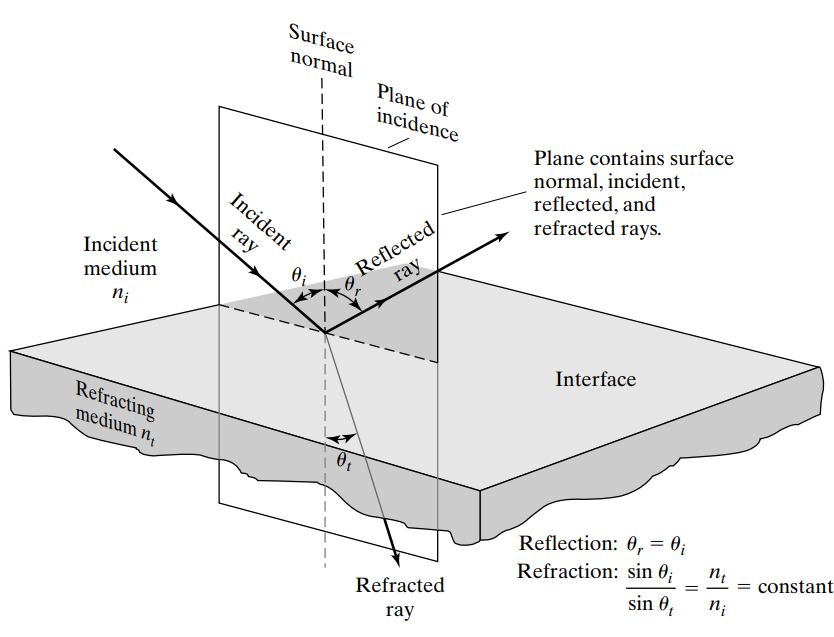
\includegraphics[scale=0.55]{Laws.png}
\end{center}

One might use Huygens' Principle to derive the laws, which proposes spherical wavelets coming out from each point of the old wavefront to form new wavefront by drawing curve tangent to all spherical wavelets in the direction of propagation, and discard parts that are not at tangent radially out. \\
\begin{center}
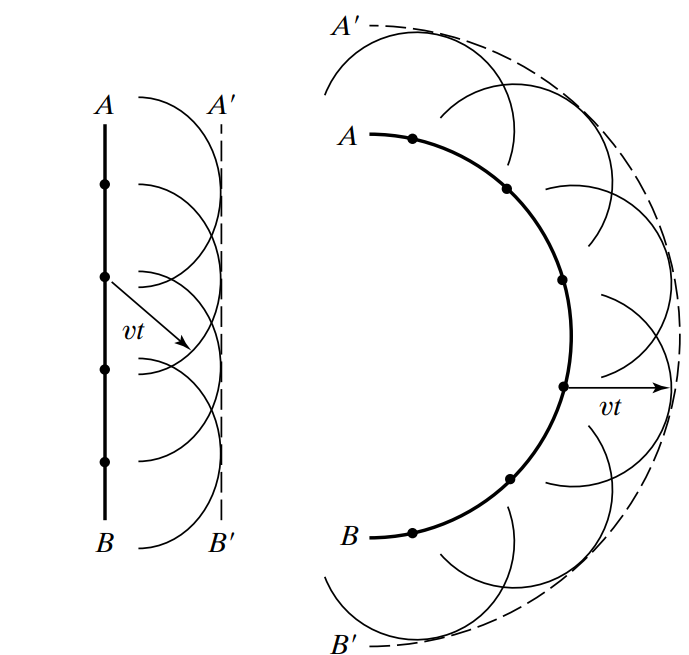
\includegraphics[scale=0.39]{Huygens.png}
\end{center}

\hfill\break
On the other hand, one might consider the Fermat Principle to derive the laws of reflection and refraction. Fermat Principle states that light takes path of the least time to travel from the starting point to the end point, which originated from Hero of Alexandria's idea that light takes the shortest path to travel.\\

Using Fermat's Principle to derive the Law of Reflection is trivial:
\begin{center}
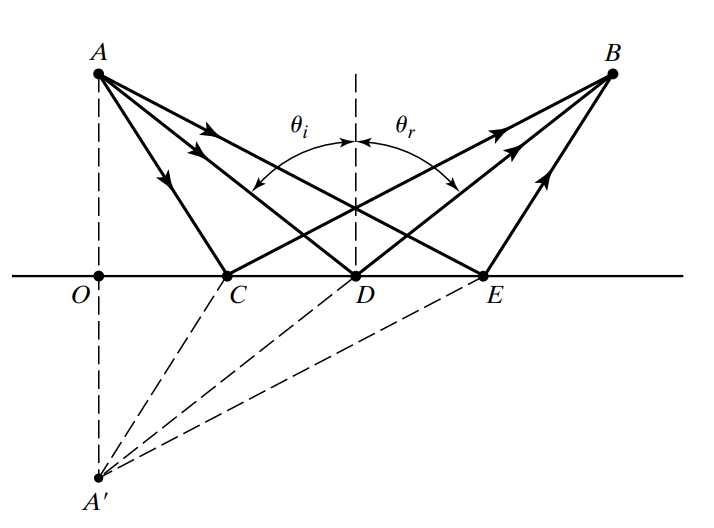
\includegraphics[scale=0.45]{Fermat1.png}
\end{center}

Using Fermat's Principle to derive the Law of Refraction requires finding extremum:
\begin{center}
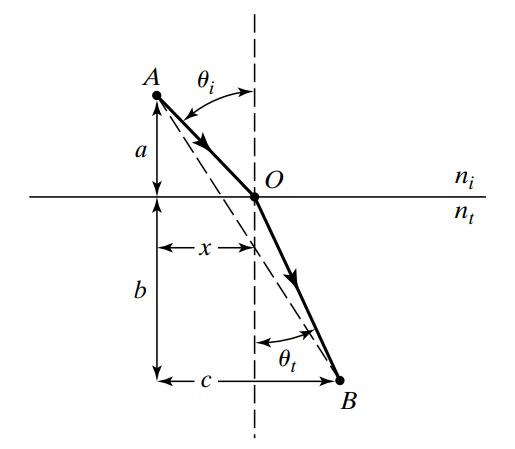
\includegraphics[scale=0.55]{Fermat2.png}
\end{center}
Let $v_i$ and $v_t$ denote the speed of the ray traveling in the two media respectively, we can write:
\begin{align*}
t = \frac{\sqrt{a^2 +x^2}}{v_i} + \frac{\sqrt{b^2 + (c-x)^2}}{v_t}
\end{align*}
we can minimize the time by setting $\frac{dt}{dx} = 0$:
\begin{align*}
\frac{dt}{dx} = \frac{x}{v_i\sqrt{a^2 +x^2}} - \frac{c-x}{v_t \sqrt{b^2 +(c-x)^2}} = 0
\end{align*}
rearranging reduces to the following:
\begin{align*}
\frac{dt}{dx} = \frac{\sin(\theta_i)}{v_i} - \frac{\sin(\theta_t)}{v_t} = 0
\end{align*}
The desired result is immediate. \\

A more precise statement of Fermat's principle, which requires merely an extremum relative to neighboring paths, may be stated as: \textit{The actual path taken by a light ray in its propagation between two given points in an optical system is such as to make its optical path equal, in the first approximation, to other paths closely adjacent to the actual one.}


\newpage
Deriving the Law of Reflection from Huygens' Principle is quite trivial:
\begin{center}
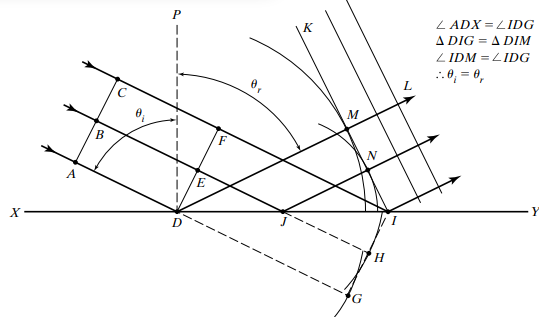
\includegraphics[scale=0.8]{HuygensRefl.png}
\end{center}

Deriving the Law of Refraction from Huygens' Principle involves accounting of the speed of the light in the refracting medium:
\begin{center}
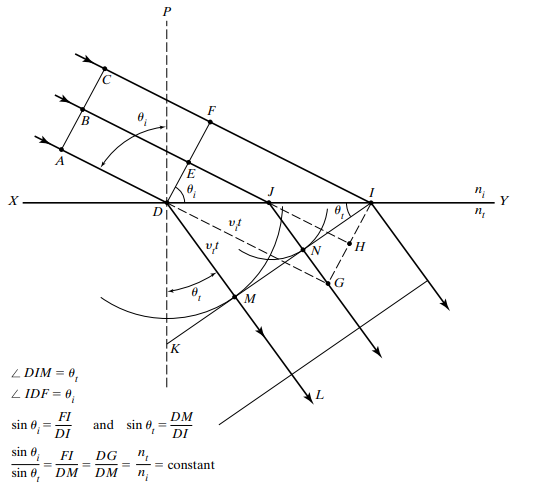
\includegraphics[scale=0.8]{HuygensRefr.png}
\end{center}

\newpage
When reversing the starting point and the ending point, Fermat's principle of least time must predict the same path as determined for the original direction of light propagation. In general, then, any actual ray of
light in an optical system, if reversed in direction, will retrace the same path backward. This is called the \textbf{Principle of Reversibility}. \\
 
 
In \textbf{specular reflection} from a perfectly smooth surface, all rays of a parallel beam incident on the surface obey the law of reflection from a plane surface and therefore reflect as a parallel beam.

In \textbf{diffuse reflection} from a granular or rough surface, though the law of reflection is obeyed locally for each ray, the microscopically granular surface results in rays reflected in various directions and thus a diffuse scattering of the originally parallel rays of light. Every plane surface will produce some such scattering, since a perfectly smooth surface can only be approximated in practice. \\

Here we note that specular reflection of a single light ray on a surface would reverse the sign of one of the coordinate component of the ray when we set up the coordinate system by using the plane surface as $xy$-, $yz$-, or $xz$-planes. Therefore, proper setup of smooth surface can make the incident ray returns precisely parallel to the line of original approach, such setup of smooth surface is usually called a corner reflector. A
network of such corner reflectors ensures the exact return of a beam of light.\\

Let $\theta_1,\theta_2$ be angle of incident and refraction, respectively, and let $n_1, n_2$ be refractive indices of incident and refraction materials, respectively. From Snell's Law, when $n_2<n_1$, the refracted rays bend away from the surface normal, and when $n_2>n_1$, on the other hand, the refracted ray bends toward the normal.\\

When rays go from medium of greater index of refraction to medium of smaller index of refraction, rays from the object that make increasingly large angles of incidence with the surface must refract at increasingly larger angles, a \textbf{critical angle of incidence} $\theta_c$ is reached when the angle of refraction reaches $90^\circ$, which can be computed from Snell's Law:
\begin{align}
\theta_c = \sin^{-1}\left( \frac{n_2}{n_1}\right)
\end{align}
For angles of incidence $\theta>\theta_c$, the incident ray experiences \textbf{total internal reflection}. For angle of incidence $\theta< \theta_c$ both refraction and reflection occur.


\newpage
\section[Imaging by Optical Systems]{\color{red}Imaging by Optical Systems\color{black}}

First we consider image formation in a plane mirror. It can be easily derived that the image size is identical with the object size, giving a magnification of unity. In addition, the transverse orientation of object and image are the same. A right-handed object, however, appears left-handed in its image.
\begin{center}
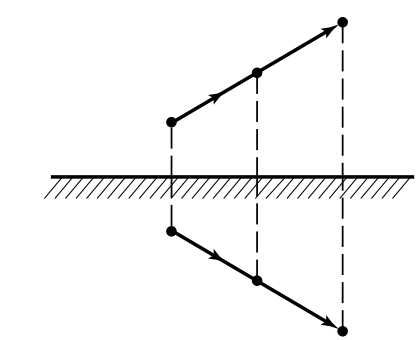
\includegraphics[scale=0.39]{mirrorIma1.png}\qquad\qquad\qquad 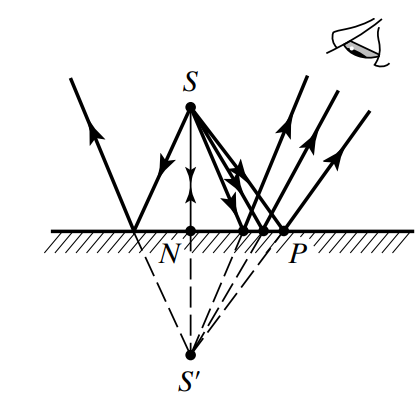
\includegraphics[scale=0.39]{mirrorIma2.png}
\end{center}

The eye sees a point image at $S'$ in exactly the same way it would see a real point object placed there. Since none of the actual rays of light lies below the mirror surface, the image is said to be a \textbf{virtual image}. The image $S'$ cannot be projected on a screen as in the case of a \textbf{real image}. Note that the image position does not depend on the position of the eye.\\

\hfill\break
When rays emerge from a lower medium of greater refractive index to an upper medium of lower refractive index, a unique image point is not determined by these rays because they have no common intersection or virtual image point below the surface from which they appear to originate after refraction. \\

\begin{center}
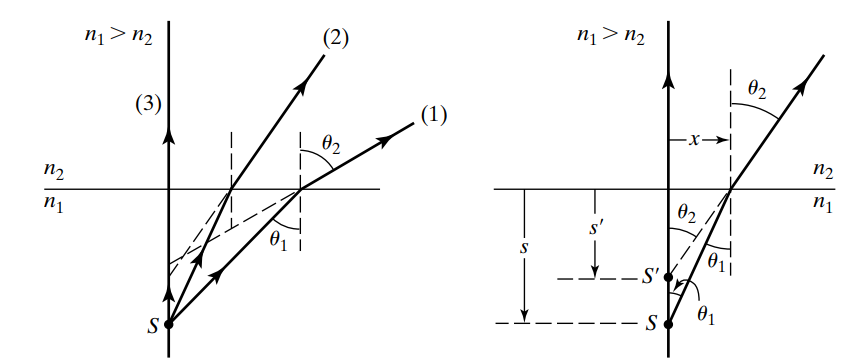
\includegraphics[scale=0.55]{refracIma.png}
\end{center}

For rays making a small angle with the normal to the surface, however, a reasonably good image can be located. In this approximation, where we allow only such paraxial rays to form the image, the angles of incidence and refraction are both small, and small angle approximation is valid. Using Snell's Law with small angle approximation, we can get:
\begin{align}
s' = \left(\frac{n_2}{n_1}\right)s
\end{align}
where $s$ is the actual vertical distance of the object in the lower medium and $s'$ is the vertical distance of the image below the surface. Thus, objects underwater,
viewed from directly overhead, appear to be nearer the surface than they actually are.


\newpage
\section[Imaging by Spherical Surfaces]{\color{red} Imaging by Spherical Surfaces\color{black}}
In this section, we will denote an object, or a source of light rays, as $O$, the image point as $I$. In an ideal optical system, every ray from $O$ intercepted by the system, and only these rays, also passes through $I$. To image an actual object, this requirement must hold for every object point and its conjugate image point. By Fermat Principle, all light rays have the same optical path length, that is, they travel to the image point from the object point using the same amount of time. The points $O$ and $I$ are said to be conjugate points for the optical system. \\

In practice, we only have non-ideal images. The \textbf{non-ideal} properties come from the (1) aberrations, (2) scattering, and (3) diffraction. \begin{enumerate}[topsep=3pt,itemsep=-1ex,partopsep=1ex,parsep=1ex]
\item Some rays leaving $O$ do not reach $I$ due to reflection losses at refracting surfaces, diffuse reflections from reflecting surfaces, and scattering by inhomogeneities in transparent media. Loss of rays by
such means merely diminishes the brightness of the image.
\item Some of rays are scattered through $I$ from nonconjugate objects, degrading the image. When the optical system itself cannot produce the one-to-one relationship between object and image rays required for perfect imaging of all object points, we speak of system \textbf{abberatoin}. 
\item The effect of using a limited portion of the wavefront leads to diffraction
and a blurred image, which is said to be \textbf{diffraction limited}.
\end{enumerate} 
Surfaces that give perfect images are called the \textbf{Cartesian Surfaces}. \\



For refractive surface, suppose the object is placed in a medium with index of refraction $n_o$, and the image point is in a medium with index of refraction $n_i$. \\

\begin{center}
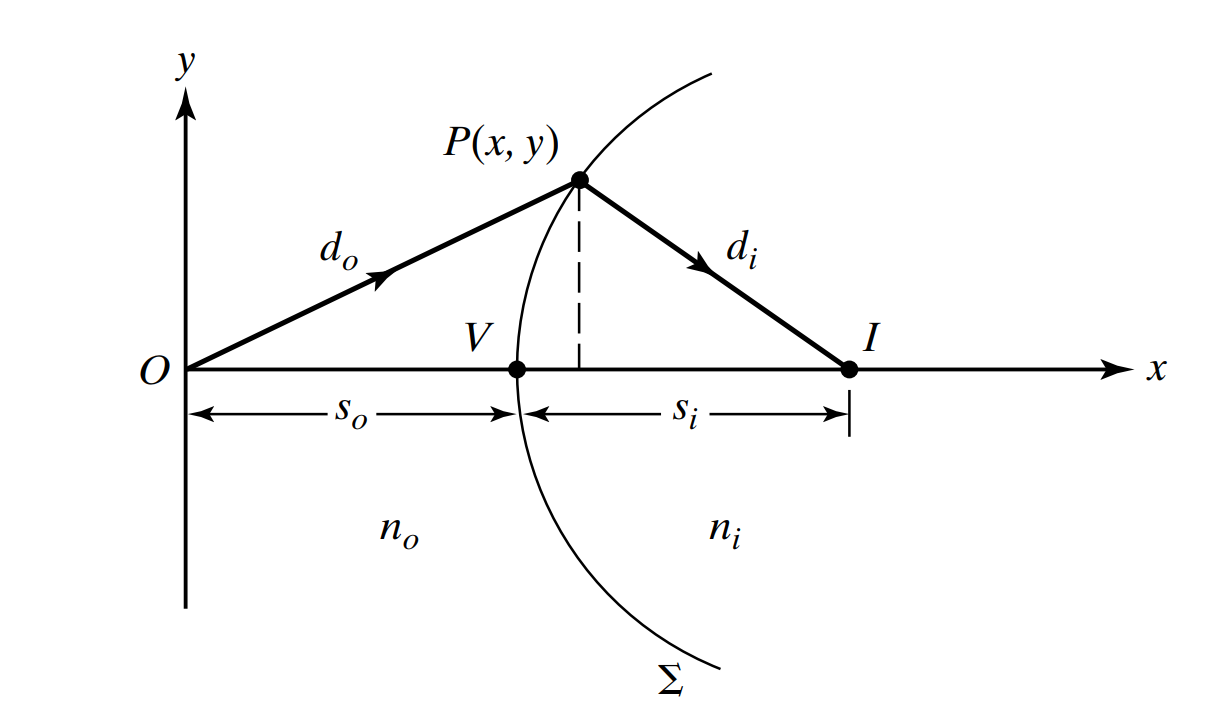
\includegraphics[scale=0.3]{catesianSurfaces.png}
\end{center}

Denote the distance between the object and the surface as $S_o$, and distance between the image point and the surface as $S_i$, then we can write, by Fermat Principle:
\begin{align*}
t = \frac{x}{v} = \frac{nx}{c} 
\end{align*}
where $nx$ is the \textbf{optical path length} taken by the light ray in a medium with index of refraction $n$, hence at any point $P$ on the surface:
\begin{align*}
n_o d_o + n_1 d_1 = n_o S_o + n_i S_i = \text{constant}
\end{align*}
In terms of the Cartesian coordinates of $P = (x,y)$, we get:
\begin{align*}
n_o (x^2+y^2)^{1/2} + n_i (y^2 + (S_o+S_i - x)^2)^{1/2} = \text{constant}
\end{align*}
Here the $\text{constant}$ in the equation is determined by $n_oS_o + n_i S_i$, which can be calculated once the specific problem is defined.\\

Note that the aberration-free imaging so achieved applies only to object point $O$
at the correct distance from the lens and on axis. For nearby points, imaging is not perfect. The larger the actual object, the less precise is its image. Because images of actual objects are not free from aberrations and because hyperboloid surfaces are difficult to grind exactly, most optical surfaces are spherical. The spherical aberrations so introduced are accepted as a compromise when weighed against the relative ease of fabricating spherical surfaces.

\hfill\break
\subsection*{Reflection from spherical mirrors}
For concave, or convex, mirrors, the reflected rays are diverging, hence forming a virtual image as if the light rays were coming from inside the surface. 
\begin{center}
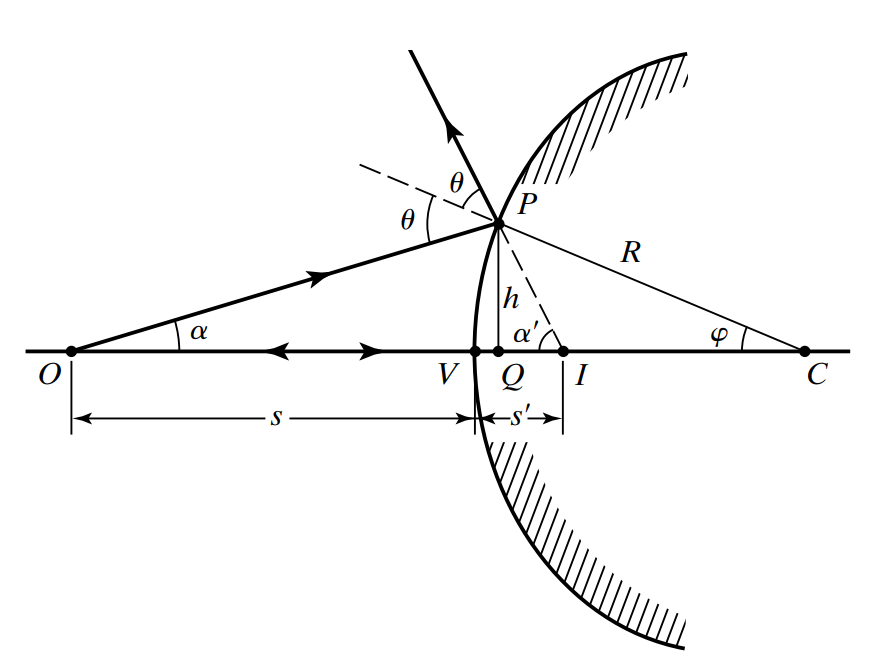
\includegraphics[scale=0.35]{reflectiveSur.png}
\end{center}

The location of the image can be found by drawing a ray $OI$ perpendicular to the surface, and a ray that strikes point $P$ on the surface, denoted as $OP$, gets reflected, the reflected ray is denoted as $IP$, extend $IP$ into the surface, and the intersection of $PI$ and $OI$ is where the virtual image is formed. Through the figure, $\theta = \alpha +\phi$, and $2\theta = \alpha + \alpha'$, hence using small angle approximation, and $VI \approx QI$, we can write:
\begin{align}
\frac{1}{s}+\frac{1}{s'} = -\frac{2}{R}
\end{align}
where we also employ some sign convention: \begin{enumerate}[topsep=3pt,itemsep=-1ex,partopsep=1ex,parsep=1ex]
\item $s>0$ implies the object point $O$ is to the left of the surface.
\item $s'>0$ implies the image point $I$ is to the left of the surface.
\item $R>0$ implies $C$ is to the right of the surface, that is the surface is convex.
\end{enumerate}
If $s,s'$ are positive, then we have real object and real image. If $s,s'$ are negative, then we have virtual objects and virtual image. For $s \to \infty$, from (2.4), we then write:
\begin{align}
f\coloneqq \frac{1}{s'} = -\frac{2}{R}\quad \begin{cases}  \text{positive for concave surfaces} \\ \text{negative for convex surfaces} \end{cases}
\end{align}

From (2.4) and the geometry of the system:
\begin{center}
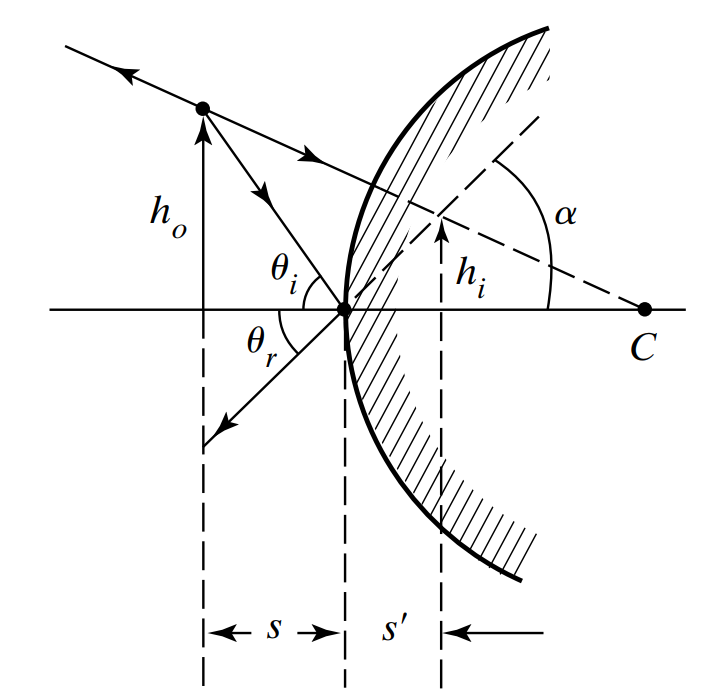
\includegraphics[scale=0.33]{reflectiveMag.png}
\end{center}
one can also derive the magnification of the image:
\begin{align}
|m| \coloneqq \frac{h_i}{h_o} = \left|\frac{s'}{s}\right|
\end{align}
where we employ the sign convention: \begin{enumerate}[topsep=3pt,itemsep=-1ex,partopsep=1ex,parsep=1ex]
\item $m>0$ for image that has same orientation as object.
\item $m<0$ for image that is inverted.
\end{enumerate}
Hence, being consistent with (2.4), we write:
\begin{align}
m = -\frac{s'}{s}
\end{align}

\hfill\break
\hfill\break
\begin{center}
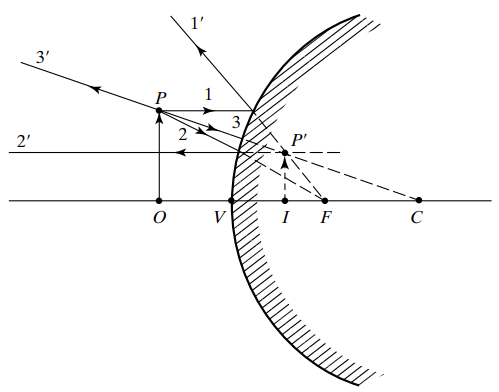
\includegraphics[scale=0.42]{drawRefle.png}
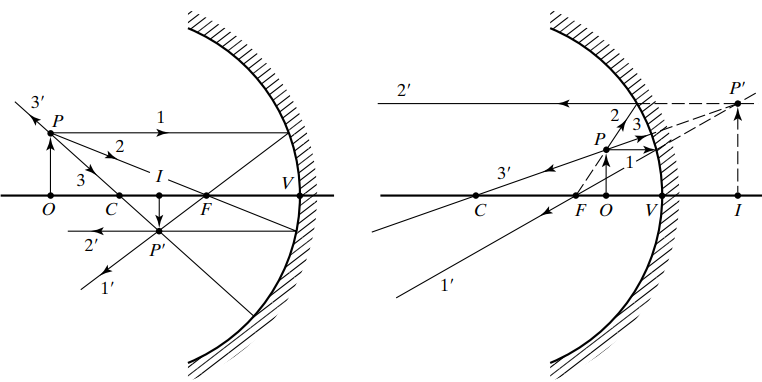
\includegraphics[scale=0.42]{drawRefle1.png}
\end{center}

\newpage
\example
A $3\, cm$ object is $20\, cm$ away from a convex spherical mirror with $f = -10\, cm$. Here we can write $R = 20\, cm$, and $s = 20\, cm$. Then we get:
\begin{align*}
\frac{1}{s}+\frac{1}{s'} = \frac{1}{f} \qquad\Rightarrow \qquad s'=\frac{sf}{s-f} = \frac{(-10)(20)}{20 +10}\, cm = \frac{200}{30}\, cm
\end{align*}
and the magnification is given by:
\begin{align*}
m = -\frac{s'}{s} = \frac{-6.67}{20} = \frac{1}{3}
\end{align*}
For concave spherical surface $20\, cm$ away with $f = 10\, cm$, we write:
\begin{align*}
s' = \frac{fs}{s-f} = \frac{(10)(20)}{20-10} = 20\, cm
\end{align*}
and the magnification is given by:
\begin{align*}
m = -\frac{s'}{s} =- \frac{20}{20} = -1
\end{align*}
\hfill\break
\hfill\break

\subsection*{Refraction by spherical surfaces}
By Snell's Law, we write:
\begin{align*}
n_1 \sin(\theta_1) = n_2 \sin(\theta_2)
\end{align*}
From the geometry in our settings:
\begin{center}
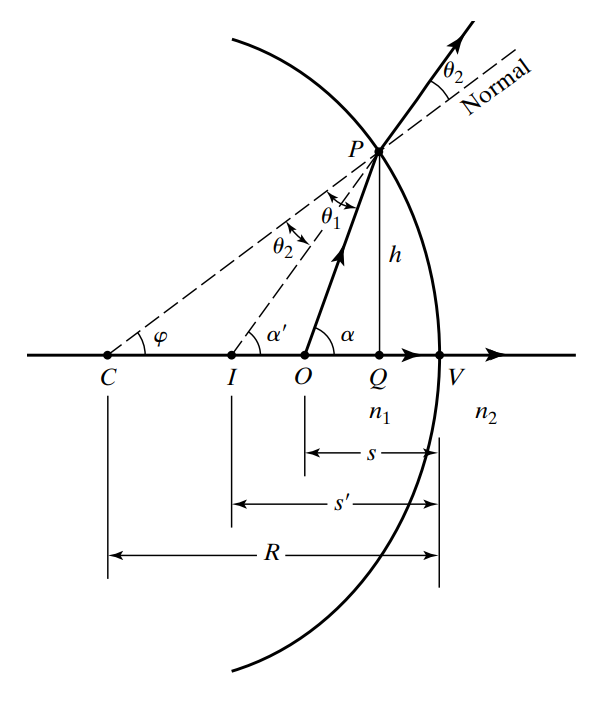
\includegraphics[scale=0.45]{refracSur.png}
\end{center}

we can write:
\begin{align*}
\alpha = \theta_1 + \phi \qquad\qquad \alpha' = \theta_2 + \phi
\end{align*}
using paraxial approximation and Snell's Law, we can write:
\begin{align*}
n_1(\alpha - \phi) = n_2(\alpha' - \phi)
\end{align*}
Ignoring the length of $QV$, and using small angle approximation, we can write:
\begin{align*}
n_1 \left( \frac{h}{s} - \frac{h}{R} \right) = n_2 \left( -\frac{h}{s'} - \frac{h}{R}\right)
\end{align*}
where we use the sign conventions for $s$ and $s'$ and $R$:
\begin{enumerate}[topsep=3pt,itemsep=-1ex,partopsep=1ex,parsep=1ex]
\item $s>0$ implies the object point $O$ is to the left of the surface.
\item $s'>0$ implies the image point $I$ is to the left of the surface.
\item $R>0$ implies $C$ is to the right of the surface, that is the surface is convex.
\end{enumerate}
rearranging we get:
\begin{align}
\frac{n_1}{s} + \frac{n_2}{s'} = \frac{n_2 - n_1}{R}
\end{align}
Using Snell's Law, (2.8), and the geometry: 
\begin{center}
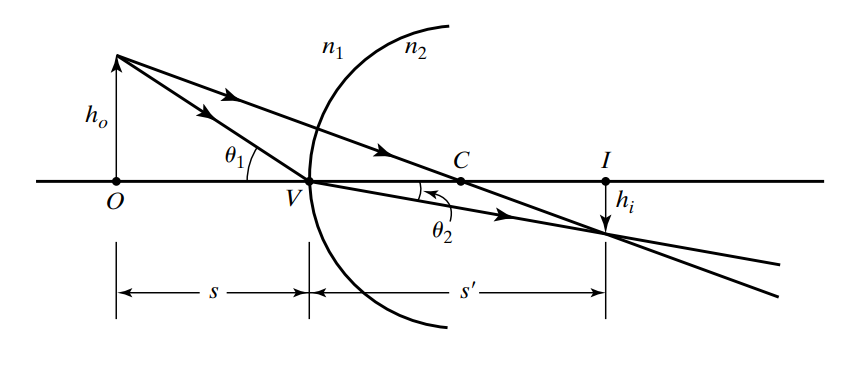
\includegraphics[scale=0.46]{refracMag.png}
\end{center}
one can get the magnification under refraction as the following:
\begin{align*}
m = \frac{h_i}{h_o} = -\frac{n_1 s'}{n_2 s}
\end{align*}



\newpage
\section[Thin Lens]{\color{red}Thin Lens\color{black}}
A \textbf{thin lens} is an optical system consisting of two spherical surfaces, which is thin enough so that we can neglect the distance between the surfaces, and assume the same index of refraction on both sides of the lens. Consider the lens itself has index of refraction $n_2$, and the medium outside the lens has index of refraction $n_1$, let $s_1, s_2$ denote the object distance from the first and second lens, $s_1', s_2'$ denote the image distance formed by the first and second lens respectively, then the first surface reads:
\begin{align*}
\frac{n_1}{s_1} + \frac{n_2}{s_1'} = \frac{n_2-n_1}{R}
\end{align*}
the second surface reads:
\begin{align*}
\frac{n_2}{s_2} + \frac{n_1}{s_2'} = \frac{n_1-n_2}{R_2} 
\end{align*}
By assumption, the distance $t$ between the surfaces is small enough to be neglected:
\begin{align*}
s_2 = t-s_1' \approx -s_1'
\end{align*}
combining we get:
\begin{align*}
\frac{n_1}{s_1} + \frac{n_1}{s_2'} = (n_2-n_1)\left( \frac{1}{R_1} - \frac{1}{R_2}\right)
\end{align*}
dropping the subscripts for the object and image distances, let $s$ denote the object distance from the thin lens and $s'$ denote the image distance from the thin lens, we get:
\begin{align*}
\frac{1}{s}+ \frac{1}{s'} = \frac{n_2-n_1}{n_1}\left( \frac{1}{R_1} - \frac{1}{R_2}\right)\coloneqq \frac{1}{f}
\end{align*}

\hfill\break
\begin{center}
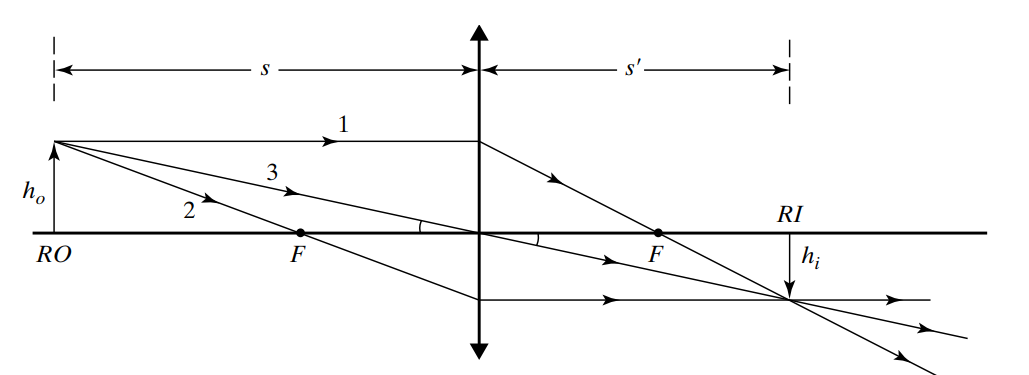
\includegraphics[scale=0.43]{concave.png}\\
\hfill\break
\hfill\break
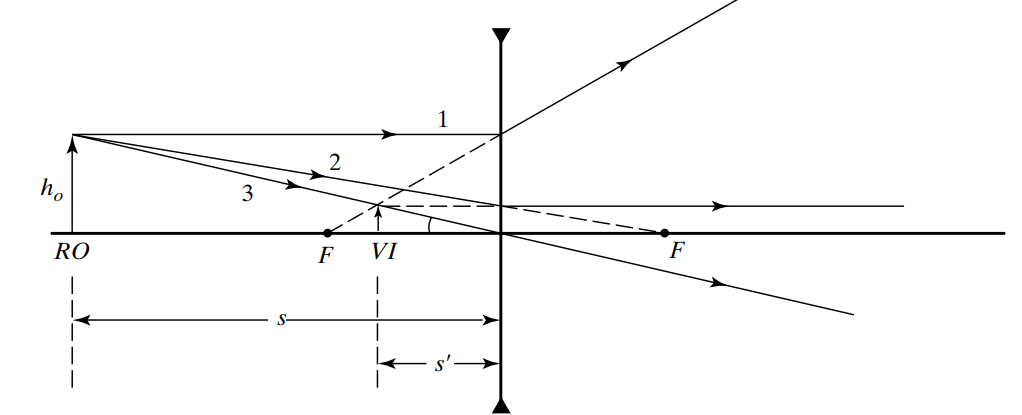
\includegraphics[scale=0.43]{convex.png}
\end{center}

For magnification, we can write the following:
\begin{align*}
\frac{h_o}{s}=\frac{h_i}{s'} \qquad \Rightarrow \qquad |m| =\left|\frac{h_i}{h_o}\right| =\left|\frac{s'}{s}\right|
\end{align*}
using sign convention, we write:
\begin{align}
m = -\frac{s'}{s}
\end{align}

\example We have a convex and a concave lens with $f = 15\, cm$, separated by $60\, cm$. The object is $25\, cm$ from the fist lens, which is the convex lens. For the image generated by the first lens, we can write:
\begin{align*}
\frac{1}{s_1}+ \frac{1}{s_1'} = \frac{1}{f} \qquad \Rightarrow s'_1 = \frac{s_1 f}{s_1- f} = \frac{25\cdot 1.5}{25-15}\, cm = 37.5\, cm
\end{align*}
and we get the magnification under the first lens:
\begin{align*}
m_1 =- \frac{s_1'}{s_1} = \frac{37.5}{25} = 1.5
\end{align*}
here $s_2 = (60-37.5) \, cm = 22.5\, cm$. Now we can calculate the image distance from the second lens:
\begin{align*}
s_2' = \frac{s_2 f}{s_2 - f} = \frac{22.5 \cdot (-15)}{(22.5)-(-15)} = \frac{337.5}{37.5} = -9\, cm
\end{align*}
and the magnification under the second lens is given by:
\begin{align*}
m_2 = -\frac{s_2'}{s_2} = \frac{-9}{22.5} = 0.4
\end{align*}
the total magnification is given by:
\begin{align*}
m = m_1 \cdot m_2 = -1.5\cdot 0.4 = -0.6
\end{align*}


\newpage
\section[Vergence and Refractive Power]{\color{red}Vergence and Refractive Power\color{black}}
For refracting surfaces, the \textbf{vergence} of a an object, or an image, is defined to be:
\begin{align*}
V = \frac{1}{s}
\end{align*}
where $s$ is the distance from the object, or the image, to the reflecting, or refracting surface. The \textbf{refractive power} of the surface is defined to be:
\begin{align*}
P = \frac{1}{f}
\end{align*}
Now let $V$ denote the vergnece of an object, and let $V'$ denote the vergence of the image of the object, we get the following:
\begin{align*}
V+V' = P
\end{align*}
Note that $P$ adds if the refractive surfaces, or the lens, are back to back, that is:
\begin{align*}
P = \sum_{i=1}^N P_i
\end{align*}
Consider a lens, let $x$ be the distance from the object to the focal point of a lens in the object space, let $x'$ be the distance from the image to the focal point of the lens in the image space, then we can write the \textbf{Newtonian equation for thin lens}:
\begin{align*}
\frac{h_i}{h_o} = \frac{f}{x} = \frac{x'}{f}
\end{align*}
Introducing a negative sign for the magnification, due to the inverted image, we write:
\begin{align*}
m = -\frac{f}{x} = -\frac{x'}{f}
\end{align*}
and for thin lens, we write:
\begin{align*}
xx' = f^2
\end{align*}

\newpage
\subsection*{Conclusion}

For surface reflection, concave surface has $f>0$ and $R<0$, convex surface has $f<0$ and $R>0$. We also write the following:
\begin{align*}
\frac{1}{s} + \frac{1}{s'} = \frac{1}{f} =-\frac{2}{R} \qquad \qquad \qquad m=-\frac{s'}{s}
\end{align*}
For surface refraction, concave surface has $R<0$, and convex surface $R>0$. We also write the following:
\begin{align*}
\frac{n_1}{s}+ \frac{n_2}{s'} = \frac{n_2- n_1}{R} \qquad \qquad\qquad m=-\frac{n_1}{n_2} \frac{s'}{s}
\end{align*}
For thin lens, concave lens has $f<0$, and convex lens has $f>0$, we also write:
\begin{align*}
\frac{1}{s}+\frac{1}{s'} = \frac{1}{f} =\frac{n_2-n_1}{n_1}\left( \frac{1}{R_1} - \frac{1}{R_2}\right) \qquad\qquad\qquad m=-\frac{s'}{s}
\end{align*}

\newpage
\section[Cylindrical Lenses]{\color{red}Cylindrical Lenses\color{black}}
The optical axis for a spherical lens is an axis of symmetry since rotation of the lens through an arbitrary angle about the optical axis leaves the lens looking just as it did before the rotation. Because the orientation of the surface curvature does not change in such a rotation, its optical behavior remains unchanged. This rotational symmetry simplifies the analysis of the imaging properties of such a spherical lens. 
\begin{center}
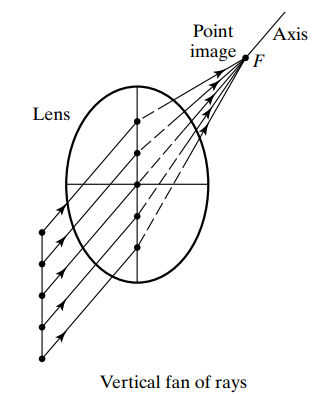
\includegraphics[scale=0.65]{sphereSym.png}\quad
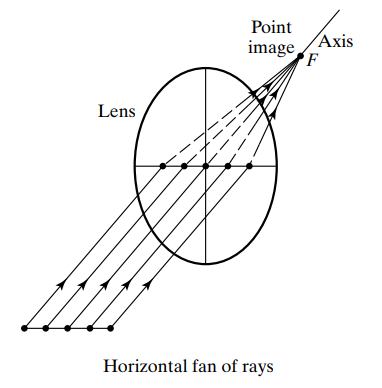
\includegraphics[scale=0.65]{sphereSym1.png}
\end{center}


On the other hand, a cylindrical lens, shaped like a section of a soft drink can, sliced down the side from top to bottom, lacks rotational symmetry about its optical axis. As a consequence, a cylindrical lens has asymmetric focusing properties. Whereas a spherical lens produces a point image of a point object, a cylindrical lens produces a line image of a point object. Because of these properties, a spherical lens is said to be \textbf{stigmatic}, and the cylindrical lens \textbf{astigmatic}. Light ray emitted by a point source will form a line image under cylindrical lens, as shown in the following:
\begin{center}
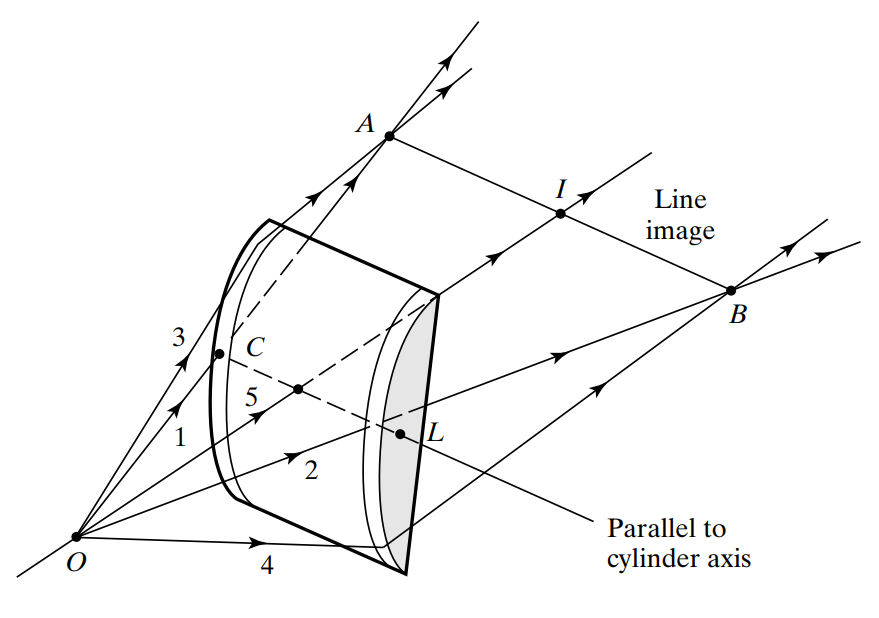
\includegraphics[scale=0.45]{cylinSym.png}
\end{center}
\newpage

The operation of the cylindrical lens is clearly asymmetric. Focusing occurs for rays along a vertical section but not for rays along a horizontal section, where the lens presents no curvature. Thus, as shown in the following figure, rays 1, 2 and 3 focus to point $A$, and rays 4, 5 and 6 focus to point $B$. However, there is no focusing of rays in a horizontal section, such as the pairs of rays 1 and 4, 2 and 5, or 3 and 6. Other vertical sections would produce other points along the focused line image AB in the same way. Notice that the line image AB so formed is always parallel to the cylinder axis.
\begin{center}
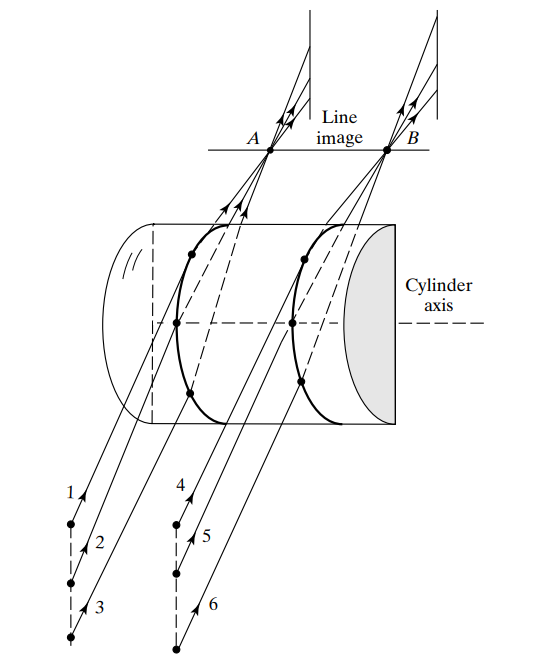
\includegraphics[scale=0.69]{cylinSym1.png}
\end{center}



\newpage
\chapter{Optical Instruments}
\setcounter{section}{5}
\section[Stops, Pupils, and Windows]{\color{red} Stops, Pupils, and Windows\color{black}}
An \textbf{aperture} is a geometric boundary due to finite size of elements, and is designed to limit to paraxial, control the amounts of light, produce a sharper outline, and cut down scattered light.\\


In particular, the aperture is used broadly to limit the field of view and control the brightness. The \textbf{aperture stop} determines the \textbf{pupils}, the entrance pupil and the exit pupil, which together control the brightness. On the other hand, the \textbf{field stop} determines the \textbf{windows}, the entrance window and the exit window, which together control the field of view.\\

The \textbf{entrance pupil} is the image of aperture stop through any preceding optical elements. The \textbf{exit pupil} is the image of the aperture stop through any following optical elements. The exit pupil matters if one system is coupled with another system.\\

The \textbf{chief ray} is the ray that passes through the center of the aperture stop, and hence also the center of the two pupils. \\

Here we note that the exit pupil is not necessarily behind the entrance pupil, and the two pupils are not necessarily located at both sides of the aperture stop. In the next page we will illustrate a simple example of locating the aperture stop and the pupils. Also notice that, when the distance between the object and the optical system changes, the aperture stop might also change, that is, an aperture stop for some objects at some distance away from the optical system might not be the aperture stop for some other objects that are closer, or further away from the system. Since the aperture stop is used to control the brightness, then by definition, the \textbf{aperture stop} is the actual physical component that limits the size of the maximum cone of rays, from an axial object point to a conjugate image point, that can be processed by the entire system. When finding the aperture stop, one needs to compute the limitation of the size of the cone generated by each physical component in the optical system. \\

The \textbf{field stop} is the real element that limits the angular field of view. The \textbf{entrance window} is the image of the field stop by preceding element. The \textbf{exit window} is the image of the field stop by following elements.  

\newpage
\hfill\break
\hfill\break
\begin{center}
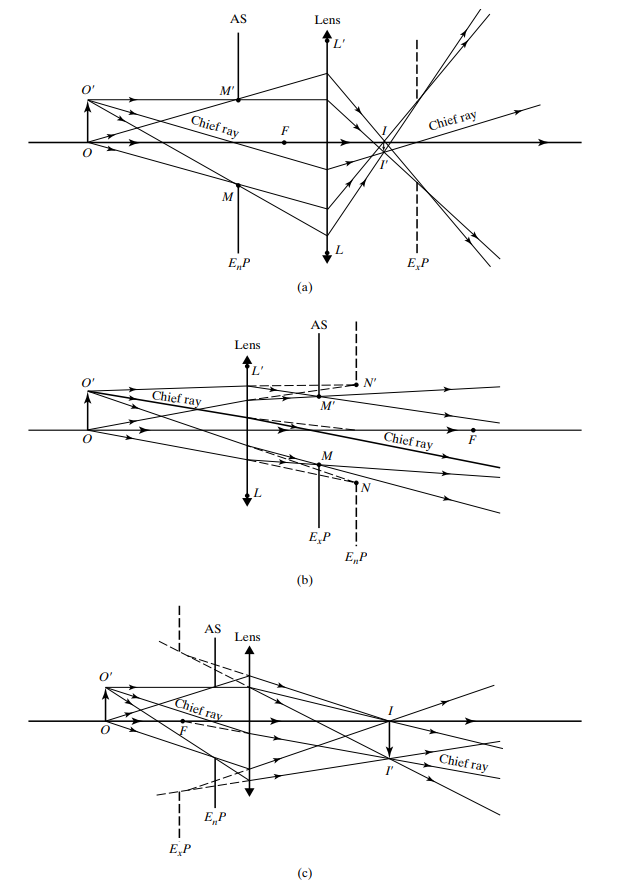
\includegraphics[scale=0.9]{pupils.png}
\end{center}
\newpage

\example Consider an object placed $15\, cm$ to the left of aperture $A$, lens $L_1$ of focal length $6\, cm$ is placed $3\, cm$ to the right of $A$, lens $L_2$ of focal length $-10\, cm$ is place $4\, cm$ to the right of $L_1$, both lens have radius $3\, cm$, and the aperture has radius $1.5\, cm$. \\

We find the $2$-dimensional angle captured by $A,\ L_1$, and $L_2$ to find the aperture stop.
\begin{align*}
\theta_A \approx \frac{1.5}{15} \approx 0.1\, rad \qquad\qquad\qquad \theta_1 \approx \frac{3}{18}\approx 0.17\, rad
\end{align*}
The position and size of the image of $L_2$ under the lens $L_1$ is given by:
\begin{align*}
\frac{1}{s}+\frac{1}{s'} = \frac{1}{f} \qquad \Rightarrow \qquad \frac{1}{4}+\frac{1}{s'_{L_2}} = \frac{1}{6} \qquad \Rightarrow \qquad s' = -12
\end{align*}
\begin{align*}
m = -\frac{s'}{s} = -\frac{12}{4} = 3 \qquad \Rightarrow \qquad h_i = 3\cdot 3\, cm = 9\, cm
\end{align*}
Clearly we have $\theta_2 > \theta_1 > \theta_A$, hence $A$ serves as an aperture stop. Hence $A$ is also itself the entrance pupil because there is no optical component preceding $A$. To get the exit pupil, we need to image $A$ through $L_1$ and $L_2$:
\begin{align*}
\frac{1}{s}+\frac{1}{s'} = \frac{1}{f} \qquad \Rightarrow \qquad \frac{1}{3}+\frac{1}{s'_{1}} = \frac{1}{6} \qquad \Rightarrow \qquad s_1' = -6\, cm
\end{align*}
\begin{align*}
\frac{1}{s}+\frac{1}{s'} = \frac{1}{f} \qquad \Rightarrow \qquad \frac{1}{(6+4)}+\frac{1}{s'_{2}} = \frac{1}{-10} \qquad \Rightarrow \qquad s_2' = -5\, cm
\end{align*}
hence the exit pupil is $5\, cm$ to the left of $L_2$. \\
The magnification of the exit pupil is given by:
\begin{align*}
m = -\frac{s'}{s} = \frac{6}{3}\frac{5}{10} = 1
\end{align*}
The location of the intermediate and final image of the object is given by:
\begin{align*}
\frac{1}{s}+\frac{1}{s'} = \frac{1}{f} \qquad \Rightarrow \qquad \frac{1}{15+3}+\frac{1}{s'_{o,1}} = \frac{1}{6} \qquad \Rightarrow \qquad s_{o,1}' = 9\, cm
\end{align*}
\begin{align*}
\frac{1}{s}+\frac{1}{s'} = \frac{1}{f} \qquad \Rightarrow \qquad \frac{1}{-5}+\frac{1}{s'_{o,2}} = \frac{1}{-10} \qquad \Rightarrow \qquad s_{o,2}' = 10\, cm
\end{align*}
and hence the final image of the object is located $10\, cm$ to the right of $L_2$. The magnification is given by the following:
\begin{align*}
m_1 = -\frac{s'_{o,1}}{s} = -\frac{1}{2} \qquad \qquad  m_2 = -\frac{s_{o,2}'}{s_2} = 2\qquad\qquad m= -\frac{2}{2} = -1
\end{align*}

\newpage
\section[Prisms]{\color{red}Prisms \color{black}}
\textbf{Aberrations} are any factor that leads to the blurring of the image form by the optical system, this includes chromatic aberration and monochromatic aberrations. For monochromatic aberrations, one talks about the spherical aberration, coma, astigmatism, field curvature, distortion, and so on. \\

\textbf{Spherical aberration} can be explained using the geometry shown in the following:
\begin{center}
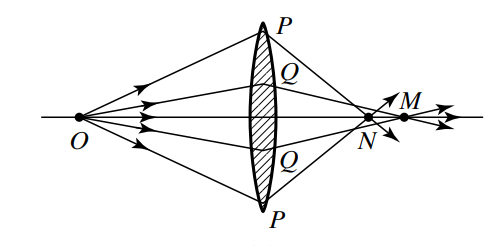
\includegraphics[scale=0.45]{sphAberr.png} \qquad 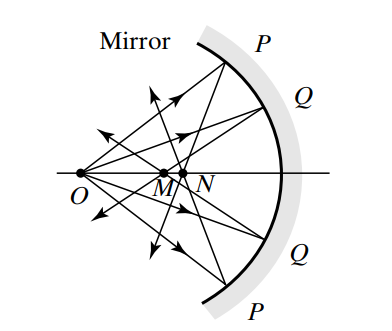
\includegraphics[scale=0.45]{sphAberr1.png}
\end{center}
To deal with spherical aberration, we can restrict the cone, use compensating negative lens, and so on.\\

The \textbf{chromatic aberration} is caused by the fact that any material has different index of refraction for different wavelength of the incident light, hence refracting the rays in different angle, causing the blurry of the image. Chromatic aberration can also be dealt by using compensating lens and so on. This effect leads to the dispersion of prisms.
\begin{center}
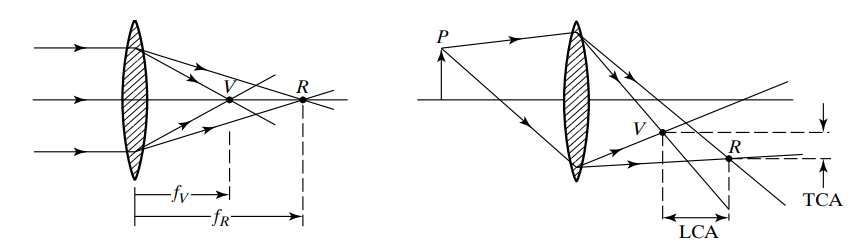
\includegraphics[scale=0.58]{chroAberr.png}
\end{center}

\hfill\break\hfill\break

We define $\delta$ to be the total angular deviation of the ray due to the action of the prism as a whole, as shown in the following:
\begin{center}
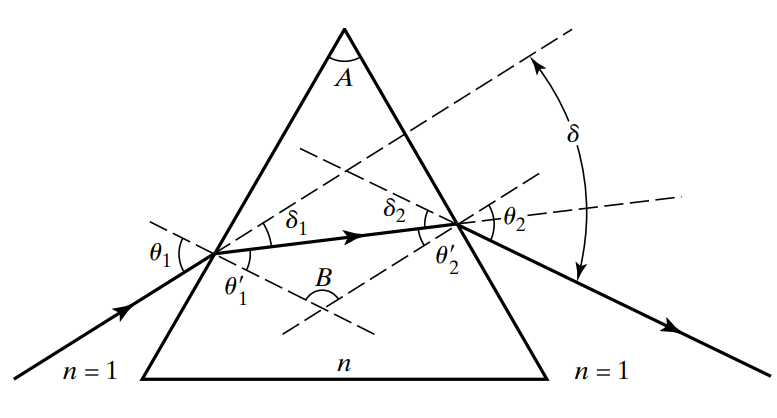
\includegraphics[scale=0.45]{prism.png}
\end{center}


where we can write:
\begin{align*}
\sin(\theta_1) &= n\sin(\theta_1')\\
n\sin(\theta_2') &= \sin(\theta_2) \\
\delta_1 &= \theta_1 - \theta_1'\\
\delta_2 &= \theta_2 - \theta_2'\\
B &= 180 - \theta_1' - \theta_2' = 180-A\\
\delta &= \delta_1 + \delta_2 = \theta_1 - \theta_1' + \theta_2 - \theta_2'
\end{align*}
Concluding we have:
\begin{align}
\delta = \theta_1 \sin^{-1}\left( n \sin\left(A-\sin^{-1}\left( \frac{\sin(\theta_1)}{n}\right) \right)\right) - A
\end{align}
For minimum deviation, we argue that when minimum deviation occurs, the ray of light passes symmetrically through the prism. Suppose this were not the case, and minimum deviation occurred for a nonsymmetrical case. Then if the ray were reversed, following the same path backward, it would have the same total deviation as the forward ray, where we see that we obtain two different minimum angle of incident, a contradiction. Hence we have $\theta_1 = \theta_2$ for minimum deviation, then we can drop the subscripts and write $\theta_1 = \theta = \theta_2$, $\theta_1' = \theta' = \theta_2'$.
\begin{center}
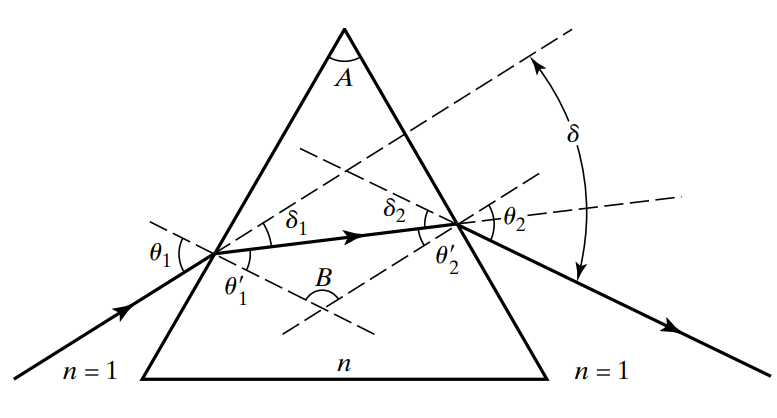
\includegraphics[scale=0.45]{prism.png}
\end{center}
in such case, we get:
\begin{align*}
\delta = 2\theta - 2\theta' \qquad \qquad A = 2\theta' \qquad\qquad \theta' = \frac{A}{2}
\end{align*}
combining we get:
\begin{align*}
\theta = \frac{\delta +A}{2}
\end{align*}
That is, combining with (3.1), we get:
\begin{align*}
n = \frac{\sin\left( \frac{A+\delta}{2}\right)}{\sin\left( \frac{A}{2}\right) }\approx \frac{A+\delta}{A} \qquad\qquad\qquad \delta \approx A(n-1)
\end{align*}

The \textbf{Dispersion} is the effect that the refraction index of a material $n$ depends on the wavelength of the light $\lambda$. Typically $n$ increases towards blue light, in which case is called the normal dispersion. If $n$ decreases towards blue, we have anomalous dispersion. The expansion relation form of $n$ is proposed by Cauchy:
\begin{align*}
n(\lambda) = A + \frac{B}{\lambda^2} + \frac{C}{\lambda^4}+ \cdots
\end{align*}
where $A,B,C \in \R$. The more applicable one is the Sellmeier formula:
\begin{align*}
n^2(\lambda) = 1+ \frac{B_1 \lambda^2}{\lambda^2 -c_1} + \frac{B_2\lambda^2}{\lambda^2 - c_2} + \cdots
\end{align*}
From Cauchy's expansion, we can write:
\begin{align*}
\frac{dn}{d\lambda} = -\frac{2B}{\lambda^3}
\end{align*}


Historically, dispersion has been characterized by using three wavelengths of light near the middle and ends of the visible spectrum. They are called 
\textbf{Fraunhofer lines}. These lines were among those that appeared in the solar
spectrum studied by J. von Fraunhofer. There are three Fraunhofer lines, the F line ($\lambda_F= 486.1\, nm$) and the C line ($\lambda_C = 656.3\,nm $) are due to absorption by hydrogen atoms, and the D line ($\lambda_D = 589.2\,nm$) is due to absorption by sodium atoms in the sun's outer atmosphere. We define the ratio of dispersion to deviation:
\begin{align*}
\Delta\coloneqq \frac{\mathcal{D}}{\delta} = \frac{n_F- n_C}{n_D - 1}
\end{align*}
$\Delta$ here is called the \textbf{Dispersive Power}, where $n_F, n_C, n_D$ are the refractive index of the three Fraunhofer lines, characterized by the material of interest. The reciprocal of the dispersive power is known as the Abbe number. \\


\begin{center}
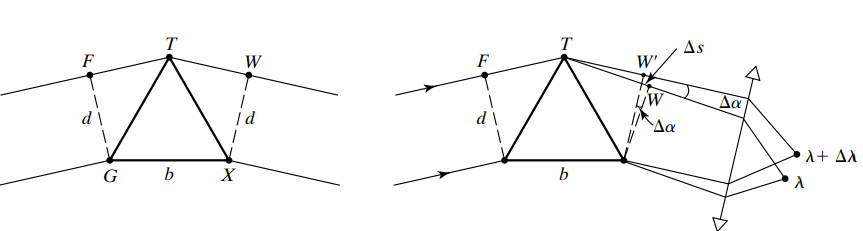
\includegraphics[scale=0.65]{resolvingPower.png}
\end{center}
By Fermat's Principle and the geometry shown, we have $FT+TW = nb$, $\lambda' = \lambda = \Delta \lambda$, $n' = n - \Delta n$. Combining we get:
\begin{align*}
FT + TW + \Delta s = (n-\Delta n)b \qquad \Rightarrow \qquad \Delta s = b \Delta n = b \frac{dn}{d\lambda}\Delta \lambda
\end{align*}
or in other words, we write:
\begin{align*}
\Delta \alpha = \frac{\Delta s}{d} = \frac{b}{d}\frac{dn}{d\lambda}\Delta \lambda
\end{align*}
where $d$ is the beam width. We appeal now to Rayleigh's criterion, which determines the limit of resolution of the diffraction-limited line images, that is the minimum separation $\Delta\alpha$ of the two wavefronts, such that the images formed are just barely resolvable:
\begin{align*}
(\Delta \alpha)_{min} = \frac{\lambda}{d}
\end{align*}
therefore combining we have:
\begin{align*}
(\Delta\lambda)_{min} = \frac{\lambda}{b\left( \frac{dn}{d\lambda}\right)}
\end{align*}
in which case we can define the \textbf{Resolving Power}, which provides a way of describing the resolution limit of the instrument:
\begin{align*}
\mathcal{R} = \frac{\lambda}{(\Delta \lambda)_{min}} =b \frac{dn}{d\lambda}
\end{align*}
Since dispersion is limited by the glass,
prism resolving power might be improved by increasing the base $b$.\\

\example Flint glass with base of $5\, cm$. We can write the following:
\begin{align*}
\frac{\Delta n}{\lambda} = \frac{1.7328 - 1.7205}{486-589} = \frac{0.0123}{-103} = 10\ee{-4}\, nm^{-1}
\end{align*}
and hence we get:
\begin{align*}
\mathcal{R} = b \left(\frac{dn}{d\lambda} \right) =( 5\ee{7}\, nm)\cdot (10\ee{-4}\, nm^{-1}) = 5\ee{3}
\end{align*}
\begin{align*}
\frac{\Delta \lambda}{\mathcal{R}} = \frac{500\, nm}{5000} = 0.1\, nm
\end{align*}

\newpage
\section[Cameras]{\color{red} Cameras\color{black}}
One can control the light power through the aperture and the shutter speed. The light power incident at the image plane, or the irradiance in watts per square meter, denoted as $E_c$, has a relation given by:
\begin{align*}
E_e \propto \frac{\text{area of aperture}}{\text{area of the image}}
\end{align*}
the image size is proportional to the focal length $f$, hence we have the relation:
\begin{align*}
E\propto \left(\frac{D}{f} \right)^2
\end{align*}
where $D$ is the circular diameter of the aperture. One can define the quantity:
\begin{align*}
A = \frac{f}{D}
\end{align*}
$A$ is called the \textbf{Relative Aperture} of the lens, also called the $f$-number or the $f$-stop. Now we can write:
\begin{align*}
E \propto \frac{1}{A^2}
\end{align*}
For conventional notation, especially in cameras, a lens with $A=k$ relative aperture is usually denoted as $f/k$.\\


\begin{center}
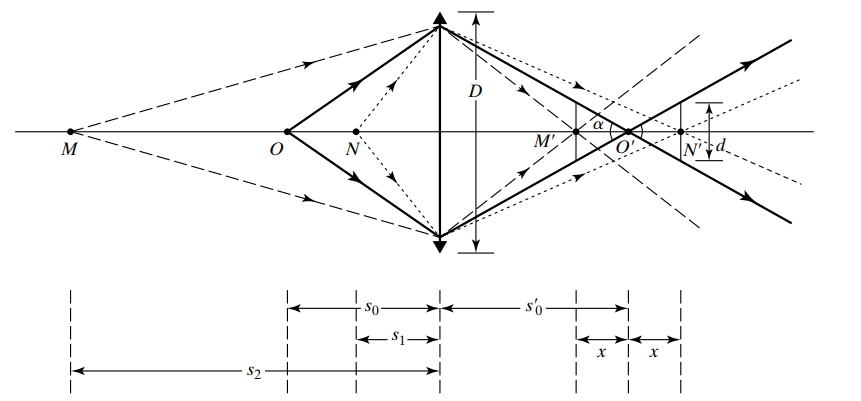
\includegraphics[scale=0.69]{dof.png}
\end{center}
Given a lens of focal length $f$, diameter $D$, and relative aperture $A = f/D$, let $d$ denote the largest acceptable diameter, let $s_0$ denote the distance from an axial object point $O$ to the lens, such that $O$ can be imaged clearly to the image point $O'$ by the lens, then the \textbf{Depth of Field} of the lens $s_2-s_1$ is around:
\begin{align*}
\text{depth of field} = \frac{2A s_0(s_0 - f)f^2}{f^4 - A^2 d^2 s_0^2}
\end{align*}
acceptable values of the circle diameter $d$ depends on the quality of the photograph desired. For most photographic work, $d$ is of the order of thousandths of an inch.\\


\newpage
\section[Simple Magnifier]{\color{red} Simple Magnifier\color{black}}
When one uses a simple magnifier, one sees a virtual enlarged image. The object needs to be placed within the focal length $f$ of the lens. A small object of height $h$, when examined by the unaided eye, is assumed to be held at the near point of the normal eye, nearest position of distinct vision, at position (a), $25\,cm$ from the eye. At this position the object subtends an angle at $\alpha_0$ the eye. To project a larger image on the retina, the simple magnifier is inserted and the object is moved physically closer to position (b), where it is at or just inside the focal point of the lens. In this position, the lens forms a virtual image subtending a larger angle $\alpha_M$ at the eye.

\begin{center}
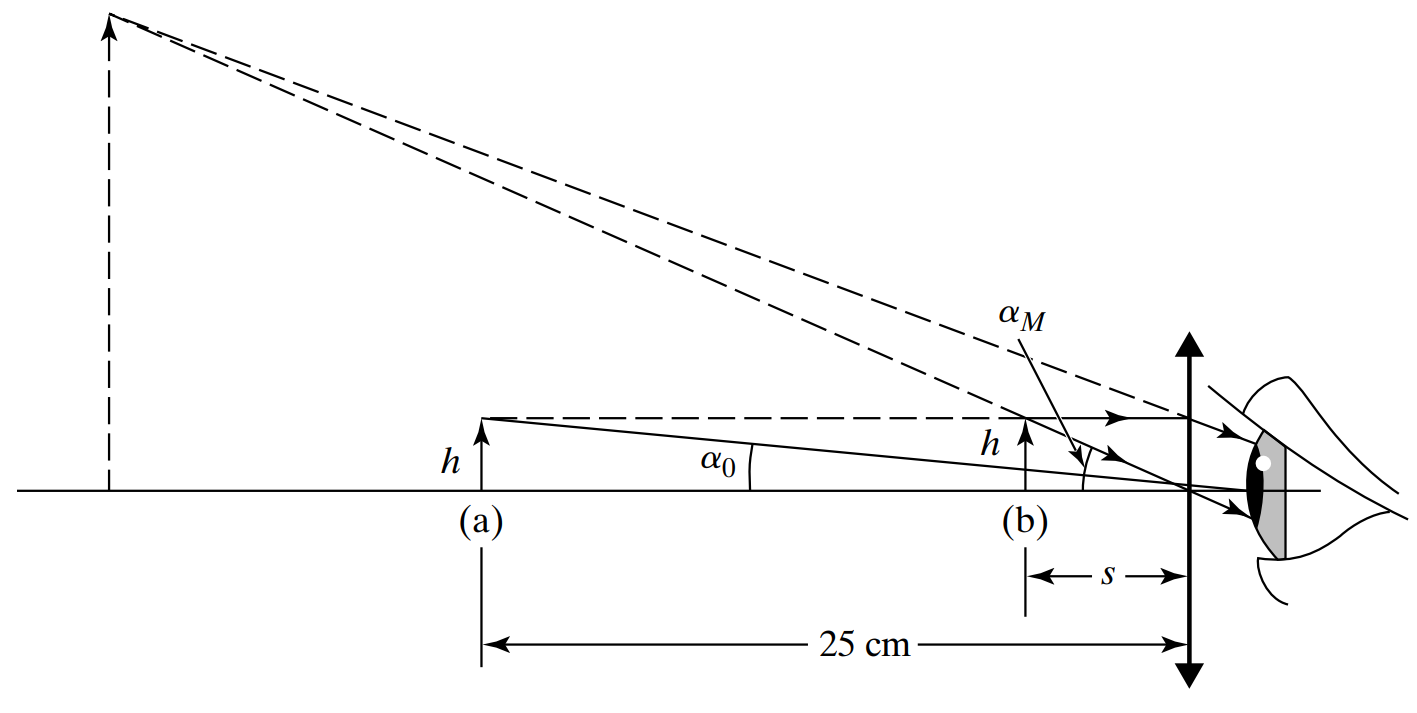
\includegraphics[scale=0.35]{magnifier.png}
\end{center}

The angular magnification of the lens can then be written as the following under paraxial approximation:
\begin{align*}
\frac{\alpha_M}{\alpha_0} \approx \frac{h/s}{h/(25\, cm)} = \frac{25}{s} 
\end{align*}
For image at distance $\infty$, we require $s = f$, hence the magnification of the lens is usually denoted as the following:
\begin{align*}
m=\frac{25}{f}\tag{Image at $\infty$}
\end{align*}
At another extreme, if the virtual image is at the nearpoint of the eye, then we require $s' = -25\, cm$, and from the thin-lens equation we get:
\begin{align*}
s = \frac{25f}{25+f}\qquad\Rightarrow \qquad m = \frac{25}{f} + 1 \tag{Image at $25\, cm$}
\end{align*}

The eyepieces of a magnifier usually consists of 2 lenses in order to reduce aberration. For two thin lens, one can derive the effect focal length $f$ by using the individual focal length $f_1$, $f_2$ of the two lenses and the distance $L$ between the lenses:
\begin{align*}
\frac{1}{f} = \frac{1}{f_1} + \frac{1}{f_2} - \frac{L}{f_1f_2}
\end{align*}
Moreover, for lenses made of the same glass of index of refraction $n$, we can write:
\begin{align*}
\frac{1}{f_1} = (n-1)\left( \frac{1}{R_{11}} - \frac{1}{R_{12}}\right) \coloneqq (n-1)K_1\\
\frac{1}{f_2} = (n-1)\left( \frac{1}{R_{21}} - \frac{1}{R_{22}}\right) \coloneqq (n-1)K_2
\end{align*}
where $R_{ij}$ is the radii of the curvature of the lenses' surface. Combining we can write:
\begin{align*}
\frac{1}{f} = (n-1)K_1 + (n-1)K_2 - L(n-1)^2 K_1K_2
\end{align*}
To correct for transverse chromatic aberration, we require that the effect focal length of the pair remain independent of the refractive index, that is:
\begin{align*}
\frac{d}{dn} \left(\frac{1}{f}\right) = 0 \tag{*}
\end{align*}
and one solution to (*) is given by:
\begin{align*}
L = \frac{1}{2}\left( \frac{1}{K_1(n-1)} + \frac{1}{K_2(n-1)}\right) = \frac{1}{2}(f_1 + f_2)
\end{align*}


\example Huygens eyepiece with $f_1 = 6.25\, cm$ and $f_2 = 2.5\, cm$. The optimum separation of the two lenses is given by the following:
\begin{align*}
L = \left( 6.25 + 2.5\right)\, cm = 4.375\, cm
\end{align*}
the equivalent focal length of the two lenses with optical separation distance is given by:
\begin{align*}
\frac{1}{f} = \frac{1}{f_1} + \frac{1}{f_2} - \frac{L}{f_1f_2} \qquad \Rightarrow \qquad f = 3.57\, cm
\end{align*}
and magnification is given by:
\begin{align*}
m = \frac{25\, cm}{f} \approx 7
\end{align*}

\hfill\break\hfill\break
For an eyepiece, we usually want angular magnification to be around $4-25$ times, and eye relief, which is distance between the eye to the exit pupil, to be around $6-26\, mm$, and we want a field of view to be around $6-30\, mm$. \\


\newpage
\section[Microscope]{\color{red} Microscope\color{black}}
The objective lens of a microscope usually has a short focal length $f_o$, and the eyepiece serves as a magnifier to magnify the object and forming virtual image so that human eye can see, with focal length $f_e$. Let $d$ denote the separation of the two lenses, the effective focal length of the microscope is given by:
\begin{align*}
\frac{1}{f_{\text{eff}}} = \frac{1}{f_o}+\frac{1}{f_e} - \frac{d}{f_of_e}
\end{align*}
hence the total magnification of the microscope is given by:
\begin{align*}
m = \frac{25(f_e + f_o - d)}{f_of_e}
\end{align*}
For the objective lens, the thin-lens equation gives:
\begin{align*}
\frac{1}{s_o} + \frac{1}{s_o'} = \frac{1}{f_o} \qquad \Rightarrow \qquad \frac{s_o'}{s_o} = \frac{s_o'}{f_o} - 1 = \frac{s_o'-f_o}{f_o}
\end{align*}
but $s_o' = d - f_e$, hence we have:
\begin{align*}
\frac{s_o'}{s_o} = \frac{d-f_e - f_o}{f_o}
\end{align*}
then we see that:
\begin{align*}
m = -\left( \frac{s_o'}{s_o}\right) \left( \frac{25}{f_e}\right)
\end{align*}
where the term $s_o'/s_o$ is the linear magnification of the objective lens, and the term $25/f_e$ is the angular magnification of the eyepiece for image at $\infty$ distance from the eye lens. \\

Consider the Newtonian formulation for microscope, let $L$ denote the distance between the focal length of the objective lens and the real image formed by the objective lens, then the magnification of the objective lens is given by:
\begin{align*}
|m_o| = \left| \frac{h_i}{h_o}\right| = \left| \frac{s_o'}{s_i}\right| = \frac{x'}{f_o} = \frac{L}{f_o}
\end{align*}
The total magnification of the microscope now reads:
\begin{align*}
 m =- \frac{25}{f_e} \frac{L}{f_o}
\end{align*}
In many microscopes, the length $L$ is standardized at $16\, cm$.\\

The light-gathering capability of the objective lens increases when increasing the refractive index in object space between the cover glass and the objective lens. A measure of this capability is the product of half-angle and refractive index, called the numerical aperture N.A.:
\begin{align*}
\text{N.A.} \coloneqq n \sin(\alpha)
\end{align*}
where $n$ is the index of refraction in the objective space, and $\alpha$ is the planer angle between the normal and the marginal light ray that is captured by the lens in the objective space. 

\begin{center}
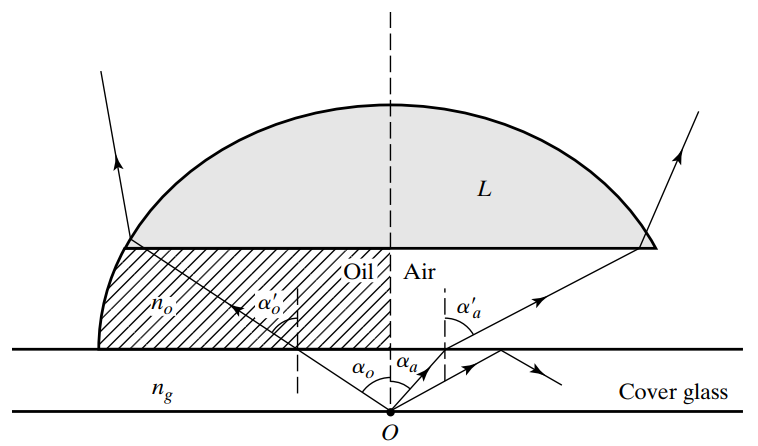
\includegraphics[scale=0.57]{NA.png}
\end{center}

Note that N.A. for an objective space is invariant. That is, in our example, in the case of air, we write:
\begin{align*}
\text{N.A.} = n_g \sin(\alpha_a) = n_{air}\sin(\alpha'_a) \approx \sin(\alpha'_a) 
\end{align*}
and in the case of oil-immersion objective is used, we write:
\begin{align*}
\text{N.A.} = n_g \sin(\alpha_o) = n_o \sin(\alpha_o')
\end{align*}




 The resolving power of a lens is proportional to N.A., and the depth of focus is inversely proportional to N.A.$^2$, typical N.A. is around $0.08-1.3$, and maximum N.A. of an objective space is $1$ in air, and $n$ in objective space filled with material with refractive index $n$. 

\newpage
\section[Telescope]{\color{red} Telescope\color{black}}
There are refractive telescopes, which uses lenses, and there are reflective telescopes, which uses mirrors. The catadioptric systems combine the refracting and reflecting telescopes.\\

For refractive telescope, there are  astronomical telescopes, which invert the images and hence have positive focal length, and there are Galilean telescope, which produces up-right image, and hence have negative focal length. The angular magnification of the refractive telescope is given by:
\begin{align*}
M = \frac{\alpha'}{\alpha} = -\frac{f_o}{f_e}
\end{align*}
and the length of the telescope is given by:
\begin{align*}
L = f_o + f_e
\end{align*}


Larger-aperture objective lenses provide greater light-gathering power and resolution. Large homogeneous lenses are difficult to produce without optical defects, and their weight is difficult to support. These problems, as well as the elimination of chromatic aberrations, are solved by using curved, reflecting surfaces in place of lenses. The largest telescopes, like the Hale 200-in. reflector on Mount Palomar, use such mirrors. Such large reflecting telescopes are usually employed to examine very faint astronomical objects and use the integrating power of photographic plates, exposed over long time intervals, in observations.
 
 
\newpage
\section[Thick Lens]{\color{red}Thick Lens\color{black}}
Consider a spherical thick lens, that is, a lens whose thickness along its optical
axis cannot be ignored without leading to serious errors in analysis. There are six \textbf{cardinal points} on the axis of a thick lens, and planes normal to the axis at these points are called the cardinal planes. Let $F_1$, $F_2$ be focal points, let $H_1$, $H_2$ be the principal points, let $N_1$, $N_2$ be the nodal points, and let $V_1$, $V_2$ be vertices of a thick lens. Distances are directed, to the left is negative, and to the right is positive. \\

A ray that passes through $F_1$ will be rendered parallel to the axis after refracted by the entire lens, and an incident ray parallel to the axis in the object space will be rendered through $F_2$ after refracted by the entire lens.  The extensions of the incident and resultant
rays in each case intersect, by definition, in the principal planes, and these cross
the axis at the principal points $H_1$ and $H_2$. If the thick lens were thin, the two principal points would coincide at the vertical line that is usually drawn to represent the lens. 
\begin{center}
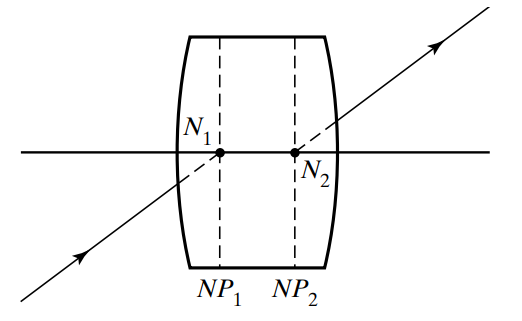
\includegraphics[scale=0.43]{nodel.png}\\
\hfill\break
\hfill\break
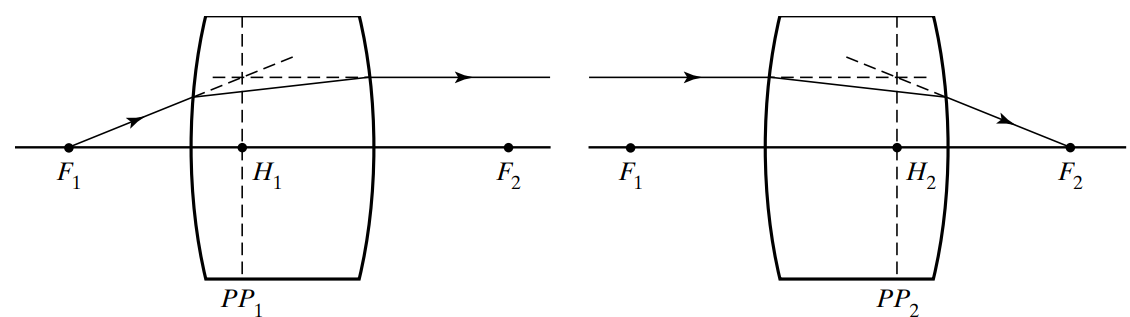
\includegraphics[scale=0.43]{principal.png}
\end{center}
Note that principal planes may be located outside the optical system itself. A incident ray that reaches $N_1$ will leave the lens at $N_2$ parallel to the the incident ray. Note here, the focal points are not measured from the vertices of the lens, they are instead measured from the principal points of the lens. 
\newpage

\begin{center}
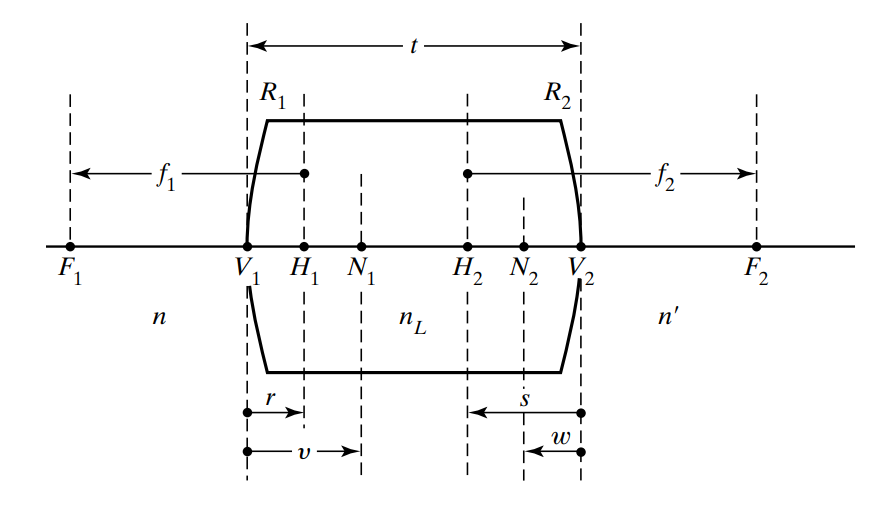
\includegraphics[scale=0.5]{thickLens.png}
\end{center}
Denote the indices of refraction in object space, the thick lens, and image space as $n, n_L, n'$, respectively, denote the radii of curvature of the lens as $R_1$ and $R_2$, and denote the thickness of the lens is $t$, then we can write the followings:
\begin{align*}
\frac{1}{f_1} = \frac{n_L- n'}{n R_2} -\frac{n_L-n}{nR_1} - \frac{(n_L-n)(n_L - n')}{n n_L} \frac{t}{R_1R_2} \qquad\qquad\qquad
f_2 = -\frac{n'}{n}f_1
\end{align*}
The principal planes can be located by computing the followings:
\begin{align*}
r = \frac{n_L - n'}{n_L R_2} f_1 t \qquad\qquad s = -\frac{n_L-n}{n_LR_1}f_2 t
\end{align*}
and the position of the nodal points is computed as the following:
\begin{align*}
v = \left( 1- \frac{n'}{n}+ \frac{n_L-n'}{n_L R_2} t\right) f_1 \qquad\qquad w = \left( 1-\frac{n}{n'} - \frac{n_L - n}{n_L R_1} t\right) f_2
\end{align*}
and together they satisfy:
\begin{align*}
-\frac{f_1}{s_o} + \frac{f_2}{s_i} = 1
\end{align*}
where for magnification, we have:
\begin{align*}
m = -\frac{ns_i}{n's_o}
\end{align*}
For lens in air, $n=n'=1$, and $r=v$, $s=w$, so we can write:
\begin{align*}
\frac{1}{s_o} + \frac{1}{s_i} = \frac{1}{f} \qquad\qquad\qquad m = -\frac{s_i}{s_o}\qquad\qquad f=f_2 = -f_1
\end{align*}

Note that $s_o$, $s_i$, $f_1$, $f_2$ are all measured from the corresponding principal planes. \\

\example\\
Consider a $4\, cm$ thick biconvex lens, with $n_L=1.52$, radii $R_1 = R_2 = 25\, cm$, at tend of cylinder water $n = 1.33$. That is, light ray goes from air to lens to water. Here we can write the following:
\begin{align*}
\frac{1}{f_1} = \frac{1.52 - 1.33}{-25} - \frac{1.52-1}{25} - \frac{(1.5-1)(1.52-1.33)}{1.52} \frac{4}{25\cdot (-25)}\, cm = -35.73\, cm
\end{align*}
\begin{align*}
f_2 = -\frac{1.33}{1}(-35.73) = 47.52\, cm
\end{align*}
\begin{align*}
r = \frac{1.52-1.33}{1.52\cdot(-25)}(-35.74)\cdot 4 = 0.715\, cm
\end{align*}
\begin{align*}
s = \frac{1.52-1}{1.52(25)}(47.53)\cdot 4 = -2.6\, cm
\end{align*}
Thus the principal point $H_1$ is situated $0.715\, cm$ to the right of the left vertex of the lens, and $H_2$ is situated $2.6\, cm$ to the left of the right vertex $V_2$. 

\newpage
\section[Matrix Methods]{\color{red}Matrix Methods\color{black}} 
Ray matrix describes optical elements by two by two matrices. Optical system is product of component matrices. The matrix method uses paraxial approximation, and describe change in heights and angle of a ray. When a light ray goes through the media of the same index of refraction, that is translation motion, its height might change but angle remains the same. While if the light ray is refracted by lenses, or reflected by surfaces, its angle would change, but height does not change. Denote the angle as $\alpha$ and height as $y$. 
\begin{center}
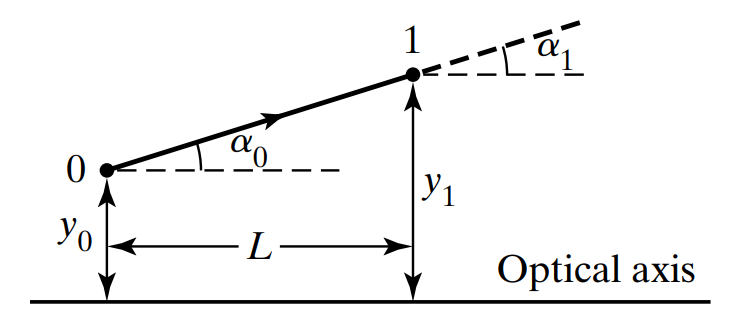
\includegraphics[scale=0.31]{trans.png}
\end{center}

For translation, we write the following:
\begin{align*}
\alpha_1 = \alpha_0 \qquad\qquad\qquad y_1 = y_0 + L \tan(\alpha_0)
\end{align*}
using small angle approximation, we can write the following:
\begin{align*}
\bmat{y_1 \\ \alpha_1} = \bmat{1 & L \\ 0 & 1} \bmat{y_0 \\ \alpha_0}
\end{align*}
where we define:
\begin{align*}
 \bmat{1 & L \\ 0 & 1}  \coloneqq \text{ray matrix for translation}
\end{align*}

\hfill\break

For refraction of spherical surface from media of refraction index $n$ to media of refraction index $n'$. We will use the following geometry:
\begin{center}
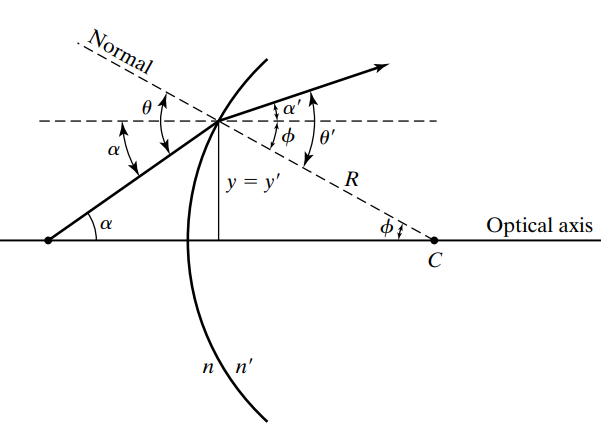
\includegraphics[scale=0.55]{refracM.png}
\end{center}
We can write the following, where we employ the sign convention $R>0$ for convex surface and $R<0$ for concave surface:
\begin{align*}
y=y' \qquad\qquad \alpha' = \phi' - \phi = \theta ' -\frac{y}{R} \qquad\qquad \alpha = \theta - \phi = \theta - \frac{y}{R}
\end{align*}
using Snell's Law and small angle approximation, we get the following:
\begin{align*}
n \theta = n'\theta' \qquad \Rightarrow \qquad \alpha'=\frac{n}{n'}\theta - \frac{y}{R} = \frac{1}{R}\left(\frac{n}{n'}-1\right) y + \frac{n}{n'}\alpha
\end{align*}
that is, we can write the following:
\begin{align*}
\bmat{y' \\ \alpha'} = \bmat{1 & 0 \\ \frac{1}{R}\left( \frac{n}{n'}-1\right) & \frac{n}{n'}}\bmat{y\\\alpha}
\end{align*}
where we define:
\begin{align*}
 \bmat{1 & 0 \\ \frac{1}{R}\left( \frac{n}{n'}-1\right) & \frac{n}{n'}} \coloneqq \text{ray matrix for refraction at spherical interface}
\end{align*}
\hfill\break


Now for reflection at spherical surface, we use the following geometry:
\begin{center}
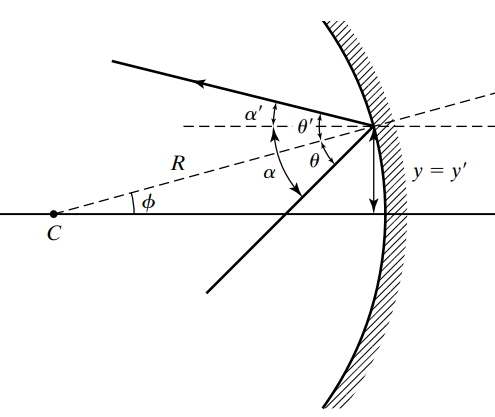
\includegraphics[scale=0.55]{reflecM.png}
\end{center}
and hence we can write the following:
\begin{align*}
y = y' \qquad\qquad\alpha = \theta + \phi = \theta + \frac{y}{-R}\qquad\qquad \alpha' = \theta' - \phi = \theta' - \frac{y}{-R} = \theta+ \frac{y}{R} = \alpha + \frac{2y}{R}
\end{align*}
hence we get:
\begin{align*}
\bmat{y' \\ \alpha'} = \bmat{1 & 0 \\ \frac{2}{R} & 1} \bmat{y \\ \alpha}
\end{align*}
where we define:
\begin{align*}
\bmat{1 & 0 \\ \frac{2}{R} & 1} \coloneqq \text{ray matrix for reflection at sperical surface}
\end{align*}

\hfill\break
\hfill\break
\example Consider a thick lens of radii of curvatures $R_1$ on the left and $R_2$ on the right. A light ray going from left to right, first through the object space of index of refraction $n$, then through the lens of index of refraction $n_L$, and finally through the image space of index of refraction $n'$. The light ray has initial angle $\alpha_0$ with respect to the axis, angle $\alpha_1$ in the lens, and angle $\alpha_3$ in the image space. Also denote the height of the ray as $y_0 = y_1$ when it intersects the first surface of the lens, and $y_2 = y_3$ at when it intersects the second surface of the lens.
\begin{center}
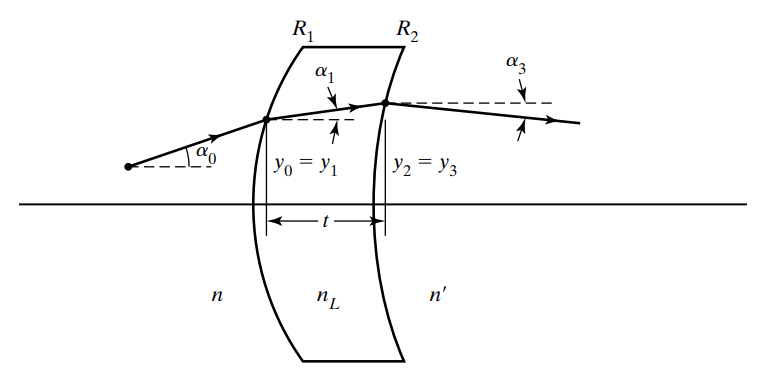
\includegraphics[scale=0.55]{matEx.png}
\end{center}

For the first refraction by the lens:
\begin{align*}
\bmat{y_1 \\\alpha_1} = M_1 \bmat{y_0 \\ \alpha_0}   
\end{align*}
For the translation in the lens:
\begin{align*}
\bmat{y_2 \\ \alpha_2} = M_2 \bmat{y_1 \\ \alpha_1 } 
\end{align*}
For the second refraction by the lens:
\begin{align*}
\bmat{y_3 \\ \alpha_3} = M_3 \bmat{y_2 \\ \alpha_2}
\end{align*}
Combining we get:
\begin{align*}
\bmat{y_3 \\ \alpha_3} = M_3M_2M_1 \bmat{y_0 \\ \alpha_0}
\end{align*}
Generalizing we can write the following:
\begin{align*}
\bmat{y_f \\ \alpha_f} = M_N M_{n-1} \cdots M_2 M_1 \bmat{y_0 \\ \alpha_0}
\end{align*}
If $\mathcal{R}_1, \mathcal{R}_2$ are ray matrices for refraction of the lens, and $\mathcal{T}$ is the ray matrix of translation in the lens, we can write $M = \mathcal{R}_2 \mathcal{T} \mathcal{R}_1$ for such thick lens. In out example, if the thickness of the lens is $t$, here we can write:
\begin{align*}
M_{\text{thick lens}} = \bmat{1 & 0 \\ \frac{n_L - n'}{n' R_2} & \frac{n_L }{n'}} \bmat{1 & t\\ 0 & 1}\bmat{1 & 0 \\ \frac{n-n_L}{n_LR_1} & \frac{n}{n_L}}
\end{align*}
for thin lens, we have $t \approx 0$, hence:
\begin{align*}
M_{\text{thin lens}} = \bmat{1& 0 \\ \frac{n_L-n}{nR_2} + \frac{n- n_L}{n'R_1}& 1} = \bmat{1 & 0 \\ \frac{n_L - n}{n}\left( \frac{1}{R_2} - \frac{1}{R_1}\right) & 1} = \bmat{1& 0 \\ -\frac{1}{f} & 1}
\end{align*}
where the last equality holds by the effective focal length for thin lens. As usual, $f$ is taken as positive for a convex lens and negative for a concave
lens.\\
\hfill\break
\hfill\break
For typical system, the ray matrix reads:
\begin{align}
M = \bmat{A&B \\C &D}
\end{align}
Note that the particular values of $M$ depend on the location of the ray at input and output. In any case, one can derive:
\begin{align*}
\det(M) = \frac{n_0}{n_f}
\end{align*}
where $n_0$ and $n_f$ are the refractive indices of the initial and final media of the optical system. Note that from theorem in linear algebra, we have:
\begin{align*}
\det(M) = \det(M_1)\cdot \det(M_2)\cdot \cdots \cdot \det(M_N) \quad\text{if}\quad M = M_1 M_2 \cdots M_N
\end{align*}

Here we discuss some significance of $A,B,C,D$ in (3.2). Consider we write the following:
\begin{align*}
\bmat{y_f \\ \alpha_f} = \bmat{A & B \\C&D} \bmat{y_0 \\ \alpha_0}
\end{align*}
then we observe that we have:
\begin{enumerate}[label=(\alph*), topsep=3pt,itemsep=-1ex,partopsep=1ex,parsep=1ex]
\item If $D = 0$, then $\alpha_f = Cy_0$, which implies the input plane is located at the first focal plane of the optical system.
\item If $A = 0$, then $y_f = B\alpha_0$, which implies the output plane is located at the second focal plane of the optical system.
\item If $B = 0$, then $y_f = Ay_0$, which implies input and output plane are object and image  plane, and $A$ gives the magnification.
\item If $C = 0$, then $\alpha_f = D\alpha_0$, which implies $D$ is the angular magnification, and we get a telescopic system.
\end{enumerate}

\begin{center}
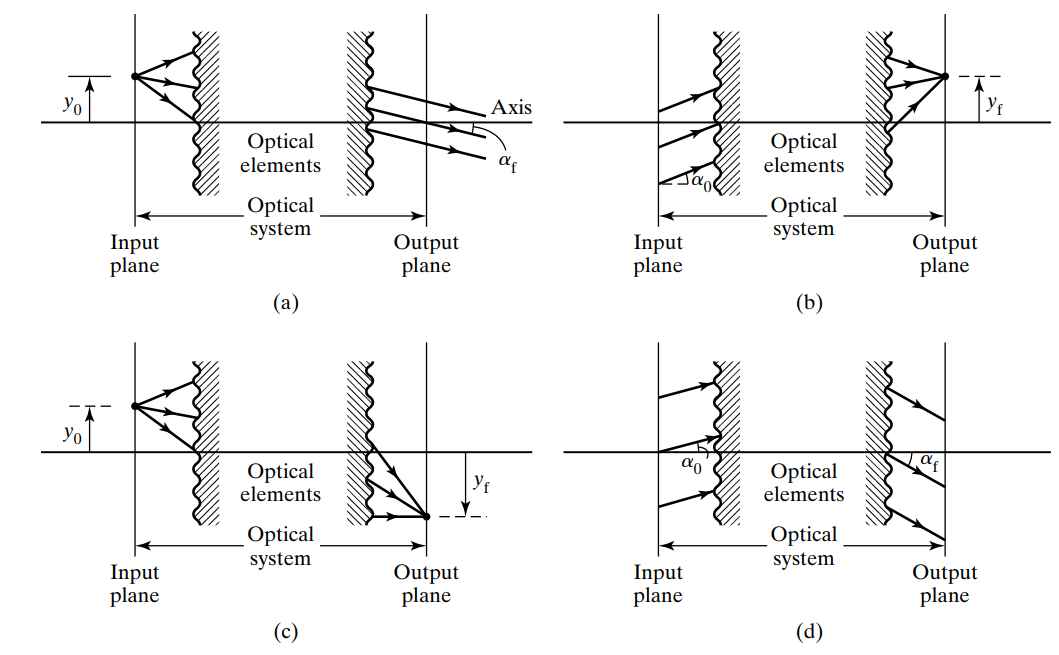
\includegraphics[scale=0.5]{ABCD.png}
\end{center}

\newpage
Now we can generalize the positions of cardinal points of an optical system by using input and output plane of the system. Here we denote the ray matrix for the entire system, with the positions of input plane and output plane well defined, as the following:
\begin{align*}
M = \bmat{A & B \\ C & D}
\end{align*}
Consider the following geometry:
\begin{center}
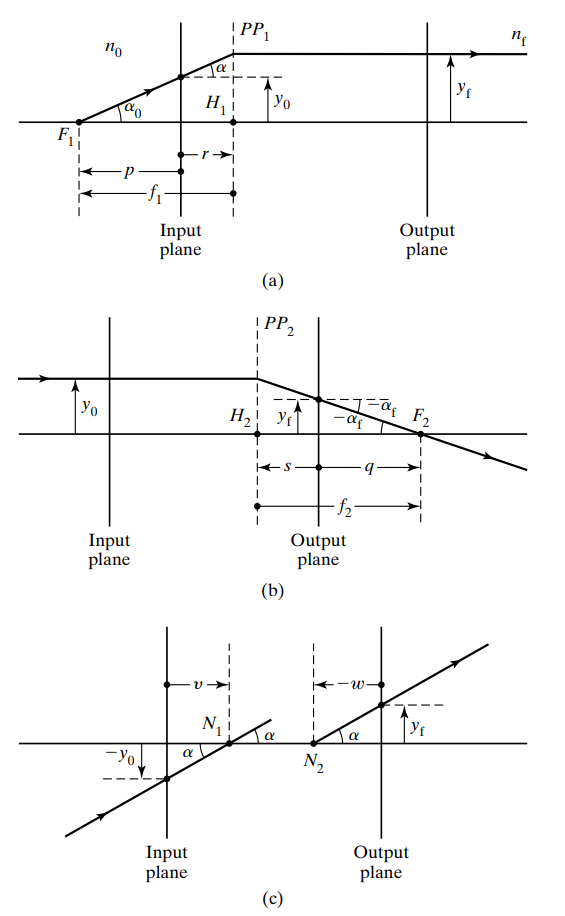
\includegraphics[scale=0.62]{sepCP.png}
\end{center}
The light ray depicted in figure (a) with initial position at the input plane $(y_0, \alpha_0)$ and final position at output plane $(y_f, \alpha_0)$ satisfies the followings:
\begin{align*}
y_f = Ay_0 + B\alpha_0 \qquad\qquad\qquad \alpha_f = Cy_0 + D\alpha_0 = 0
\end{align*}
hence we have:
\begin{align*}
y_0 = -\frac{D}{C}
\end{align*}
from small angle approximation, we get:
\begin{align*}
\alpha_0 = \frac{y_0}{-p} \qquad \Rightarrow \qquad p = -\frac{y_0}{\alpha_0} = \frac{D}{C}
\end{align*}
also, we have:
\begin{align*}
\alpha_0 = -\frac{y_f}{f_1} \qquad \Rightarrow \qquad f_1 = -\frac{y_f}{\alpha_0} = - \frac{Ay_0 +By_0}{\alpha_0} = = \frac{AD - BC}{C} = \frac{\det(M)}{C} = \frac{n_0}{n_f} \frac{1}{C}
\end{align*}
and from the geometry, we can write:
\begin{align*}
r = p-f_1 = \frac{D}{C} - \frac{n_0}{n_f} \frac{1}{C} = \frac{1}{C} \left( D - \frac{n_0}{n_f}\right)
\end{align*}
Similarly for the $q, f_2, s$, we can write the followings:
\begin{align*}
q = -\frac{A}{C} \qquad\qquad f_2 = q-s = -\frac{1}{C} \qquad\qquad s=\frac{10A}{C}
\end{align*}

For nodal points, consider the light ray in figure (c), we can write:
\begin{align*}
\alpha = -\frac{y_0}{v} = Cy_0 + D\alpha \qquad \Rightarrow \qquad \frac{y_0}{\alpha} = \frac{1-D}{C} \qquad \Rightarrow \qquad v=\frac{D-1}{C}
\end{align*}
and compute similarly for $w$:
\begin{align*}
w = \frac{\frac{n_0}{n_f}-A}{C}
\end{align*}

\begin{center}
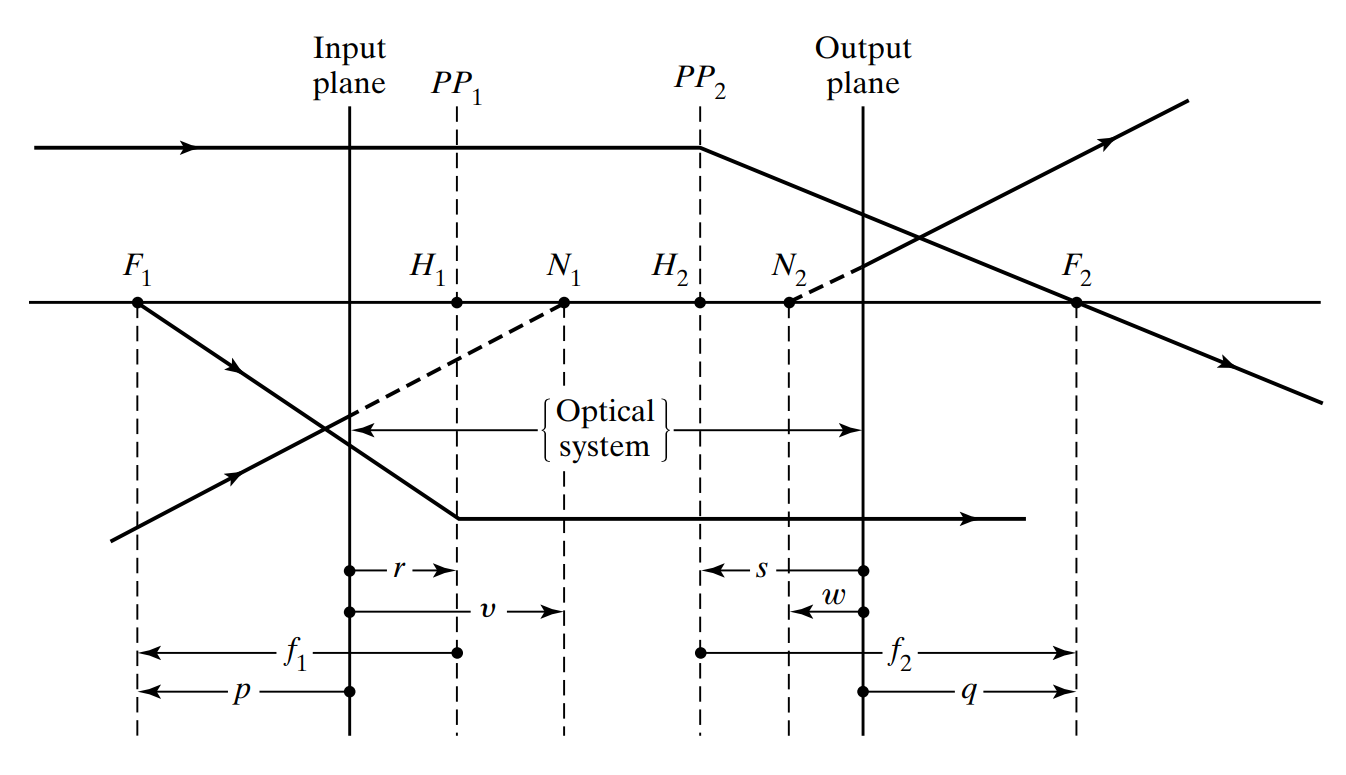
\includegraphics[scale=0.35]{oneCP.png}
\end{center}

Simple observation reveals that, if $n_0 = n_f$, then the principal points and nodal points coincide, that is we have $r=v$ and $s=w$, and we also have $f_1 = f_2$. We also see that the separation of principal points is the same as that of the nodal points, that is $r-s = v-w$.

\newpage
\example\\
Consider two thin lenses, separated by $L$, with focal lengths $f_A$ and $f_B$, the ray matrix of such system is given by the following:
\begin{align*}
M = \bmat{1 & 0 \\ 1/f_B & 1}\bmat{1 & L \\ 0 & 1} \bmat{1 & 0 \\ -1/f_A & 1}
=\bmat{1 - L/f_A &  L \\ -(1/f_B) (1-1/f_B) - 1/f_A & -L/f_B + 1}
\end{align*}
here we have:
\begin{align*}
f_1 = \frac{1}{C} \qquad \qquad \qquad f_2 = -\frac{1}{C} \qquad \qquad f_{eq} = f_2 = \frac{1}{C}
\end{align*}
hence we have:
\begin{align*}
f_{eq} =- \left( -\frac{1}{f_B} + \frac{L}{f_A f_B} - \frac{1}{f_A}\right) = \frac{1}{f_A} + \frac{1}{f_B} - \frac{L}{f_A f_B}
\end{align*}
the position of the principal and nodal points can be found:
\begin{align*}
r = v = \frac{D-1}{C} = \frac{- L/f_B + 1 - 1}{-1/f_{eq}} = -L \frac{f_{eq}}{f_B}
\qquad\qquad
s = w = -\frac{f_{eq}}{f_A} L
\end{align*}

\hfill\break
\note Making use of the $f_{eq}$, the distances of the object and image in such system is determined with respect to the principal points of the system. \\

\example 
For Huygene eyepiece, we let $f_A = 3.125\, cm$, $f_B = 2.083\, cm$, and hence $L = (1/2)(f_A + f_B) = 2.604\, cm$, where we get:
\begin{align*}
\frac{1}{f_{eq}} = \frac{1}{f_A} + \frac{1}{f_B} - \frac{L}{f_A f_B} = 0.4 \,cm^{-1} \qquad \Rightarrow f_{eq} = 2.5\, cm
\end{align*}
hence the magnification is given by:
\begin{align*}
m = \frac{25}{f_{eq}} = 10
\end{align*}
Moreover, we can write:
\begin{align*}
r = \frac{f_{eq}}{f_B}L = 3.125\, cm \qquad\qquad\qquad s = \frac{f_{eq}}{f_A}L = -2.083\, cm
\end{align*}

For an optical system, the \textbf{meridional rays} are rays that goes through the optic axis, the \textbf{skew rays} on the other hand, doe snot cross the optic axis. Almost all rays that we have been discussed in this text are meridional rays. \newpage


\chapter{Waves}
Consider a coordinate system $(x'y')$ moving at speed $v$ with respect to the coordinate system $(xy)$ in the $x$-direction. Here we have $x' = x-vt$. Let $f(x')$ be a stationary path in $(x'y')$, and here we have $f(x') = f(x-vt)$. Here we say $f$ is a wave traveling in the $x$-direction with speed $v$ in the $(xy)$ coordinate system. Mathematically, a \textbf{wave function} $f$ should satisfies the PDE given by the following:
\begin{align}
\frac{\partial^2 f}{\partial x^2} = \frac{1}{v^2}\frac{\partial^2 y}{\partial t^2}
\end{align}
(4.1) is called the \textbf{Wave Equation}. For reasonable $f(x\pm vt)$, we can write the following:
\begin{align*}
\frac{\partial f}{\partial x} = \frac{\partial f}{\partial x'}\frac{\partial x'}{\partial x} = \frac{\partial f}{\partial x'} \qquad \Rightarrow \qquad \frac{\partial^2 f}{\partial x^2} = \frac{\partial^2 f}{\partial (x')^2}
\end{align*}
\begin{align*}
\frac{\partial f}{\partial t} = \frac{\partial f}{\partial x'} \frac{\partial x'}{\partial t} = \pm v \frac{\partial f}{\partial x'} \qquad \Rightarrow \qquad \frac{\partial^2 f}{\partial t^2} = \frac{\partial}{\partial t}\left( \pm v \frac{\partial f}{\partial x'}\right) = v^2 \frac{\partial^2f}{\partial (x')^2}
\end{align*}
That is, we can write:
\begin{align*}
\frac{\partial^2 f}{\partial x^2} = \frac{1}{v^2}\frac{\partial^2 y}{\partial t^2}
\end{align*}
agrees with (4.1) that describes $1$-dimensional wave equation. Any reasonable function of the form $f(x \pm vt)$ should satisfies (4.1) as we have shown above.\\


\section[Harmonic Waves]{\color{red} Harmonic Waves}
A \textbf{harmonic wave} is of the form given by the following:
\begin{align}
f(x\pm vt) = A \sin(k(x\pm vt)) + B \cos(k(x\pm vt)) \qquad \qquad A,B \in \R
\end{align}
Note that the set of functions with coefficients $A,B \in \R$ defined by (4.2) is complete, that is we can use Fourier series of (4.2) to represent any periodic function. On the other hand, (4.2) can also be expressed as the following form:
\begin{align}
f(x\pm vt) = A \sin(k((x+\phi) + vt))  \qquad\qquad A,\phi \in \R
\end{align}
If $\lambda$ denotes the \textbf{wavelength} of the wave, then from (4.3) it is easy to see that we have:
\begin{align*}
k = \frac{2\pi}{\lambda}
\end{align*}
If $T$ denotes the \textbf{period} of the wave, we must have:
\begin{align*}
A \sin\left( k (x+v(t+T))\right) = A\sin\left( k x+kvt+2\pi\right) 
\end{align*}
and hence we get:
\begin{align*}
\frac{2\pi vT}{\lambda} = 2\pi \qquad \Rightarrow \qquad v = \frac{\lambda}{T} = \nu \lambda
\end{align*}
where $\nu$ denotes the \textbf{frequency} of the wave and satisfies $\nu = 1/T$. The \textbf{angular frequency} of the wave is given by $\omega = 2\pi \nu$, and $\kappa \coloneqq 1/\lambda$ is called the \textbf{wavenumber}. Note that $\kappa$ denote the \textbf{spacial frequency} of the wave. \\

A sinusoidal wave can be described by one of the followings, up to a phase shift:
\begin{align*}
f(x\pm vt) = A\cos(k(x\pm vt)) = A\cos\left(2\pi \left( \frac{x}{\lambda}\pm \frac{t}{T}\right) \right) = A\cos(k x \pm \omega t) 
\end{align*}
\begin{align*}
f(x\pm vt) = A\sin(k(x\pm vt)) = A\sin\left(2\pi \left( \frac{x}{\lambda}\pm \frac{t}{T}\right) \right) = A\sin(k x \pm \omega t) 
\end{align*}
where the term $\phi = k\cdot (x\pm vt)$ is called the \textbf{phase}. If $x$ and $t$ changes to keep $\phi$ constant, when the wave looks the same.\\

Method of constant phase reads the following:

\begin{align*}
d\phi = 0 = k(dx \pm v\, dt) \qquad \Rightarrow \qquad \frac{dx}{dt} = \mp v
\end{align*}
this confirms that $v$ is the \textbf{velocity} of the wave. Allowing an arbitrary initial value at $x= 0$, $t= 0$, we write the general form of a sinusoidal wave:
\begin{align*}
f(x\pm vt) = A \sin(k\cdot (x\pm vt) + \phi_0)
\end{align*}
If $f(0) = y_0$ at $x=0$, $t=0$, then $f(0) = A \sin(\phi_0)$ with $\phi_0 = \sin^{-1}(y_0/A)$. \\

\example\\
Consider the following wave: 
$$y(x,t) = (0.35\, m) \sin\left( (3\pi /m)x - (10\pi/s)t + \pi/4\right)$$ 
Then we have:
\begin{align*}
k = \frac{3\pi}{m} \qquad \qquad \qquad \omega = \frac{10\pi}{s} \qquad\qquad\qquad \lambda = \frac{2\pi}{k} = \frac{2}{3}\, m \qquad\qquad\qquad \nu = \frac{\omega}{2\pi} = 5\, Hz
\end{align*} 
The initial phase is $\pi/4$, velocity is given by $v = \lambda \nu = 3.33\, m/s$.\\

\subsection{Complex Form of Sinusoidal Waves}
The complex form of a harmonic wave can be written as the following:
\begin{align*}
\widetilde{y} = Ae^{i(kx - \omega t)}
\end{align*}
where we can extract the real part and complex part to get the sinusoidal wave:
\begin{align*}
y = \Re(\that{y}) = A \cos(kx - \omega t) \qquad\qquad\qquad y = \Im(\that{y}) = A \sin(kx - \omega t)
\end{align*}

\newpage
\subsection{Plane Waves}
A \textbf{plane wave} describes a $3$-dimensional waveform:
\begin{align*}
\Psi = A\sin(kx - \omega t)
\end{align*}  
which is a traveling wave, at fixed time, say $t=0$, we have:
\begin{align*}
\Psi|_{t=0} = A \sin(kx)
\end{align*}
here planes of constants phase $x = \text{constant}$ are wavefronts, and they travel with speed characterized by $\Psi$. Here $\Psi$ travels in the $x$- direciton, at arbitrary $\vec{r}\in \R^3$, $\vec{r}$ locates at the plane wave characterized by $x = r\cos(\theta)$, $t=0$, where $\theta$ is the angle between $\vec{r}$ and the $x$-axis, that is, we have:
\begin{align*}
\Psi = A\sin(kr\cos(\theta))
\end{align*}

To generalize this result, we generalized plane ave traveling in direction $\vec{k}$ in $\R^3$ can be written as the following, up to a phase shift:
\begin{align*}
\Psi = A \sin(\vec{k}\cdot \vec{r} - \omega t)
\end{align*}
where we have:
\begin{align*}
\vec{k}\cdot \vec{r} = x k_x + yk_y + zk_z = k r\cos(\theta) = ks
\end{align*}
where $ks $ is the component of $\vec{r}$ in the direction of $\vec{k}$, $\theta$ is the angle between $\vec{k}$ and $\vec{r}$. \\

In Complex form, we can write the following:
\begin{align*}
\that{\Psi} = Ae^{i(\vec{k}\cdot \vec{r} - \omega t)}
\end{align*}
which satisfies:
\begin{align}
\frac{\partial^2 \that{\Psi}}{\partial x^2} + \frac{\partial^2 \that{\Psi}}{\partial y^2} + \frac{\partial^2 \that{\Psi}}{\partial z^2} = \frac{1}{v^2} \frac{\partial^2 \that{\Psi}}{\partial t^2}
\end{align}
here (4.4) reads the $3$-dimensional wave equation. In other words, we have:
\begin{align*}
\nabla^2 \Psi = \left(\frac{\partial^2}{\partial x^2}+\frac{\partial^2}{\partial y^2}+\frac{\partial^2}{\partial z^2} \right) \Psi= \frac{1}{v^2} \frac{\partial^2 \Psi}{\partial t^2}
\end{align*}
Note that plane wave is not physical by energy conservation, that the planes can be extended to infinity and causes the total energy for each plane, if that has nonzero energy at some point, to diverge. 


\subsection{Spherical Waves}
Note that \textbf{spherical wave} is not physical either because $r=0$ the wave function fails. The wave function for spherical wave is given by the following:
\begin{align*}
\Psi = \left( \frac{A}{r}\right) e^{i(kr \pm \omega t)}
\end{align*}
note that $r$ denote the distance $r$ away from the origin. 

\subsection{Cylindrical Wave}
Cylindrical wave usually comes from a line source, such as plane waves passes through a slit, forming emerging cylindrical waves:
\begin{align*}
\Psi = \left(\frac{A}{\sqrt{\rho}}\right) e^{i(k\rho \pm \omega t)}
\end{align*}
where $\rho = \sqrt{x^2 + y^2}$ is the distance from the line source. Cylindrical wave is not physical either, because it diverges at $\rho=0$, and the cylindrical planes can be extended to infinity causing the energy to diverge.\\




\section[Electromagnetic Waves]{\color{red} Electromagnetic Waves\color{black}}
\textbf{Electromagnetic waves} are usually emitted by oscillating charged particles. One can writ the wave function $\Psi$ by either $\vec{E}$ or $\vec{B}$, one implies the other by Maxwell's Equations. Here $\vec{E}$ and $\vec{B}$ are perpendicular to each other, and are perpendicular to the propagation direction $\vec{k}$:
\begin{align*}
\vec{E} = \vec{E}_0\sin(\vec{k}\cdot \vec{r} -\omega t) \qquad\qquad &\text{electric field}\\
\vec{B} = \vec{B}_0 \sin(\vec{k}\cdot \vec{r}- \omega t)\qquad\qquad &\text{magnetic field}
\end{align*}
where $\vec{E}_0$ and $\vec{B}_0$ characterize the magnitude of the wave, and from Maxwell's Equations, we have $E_0 = c B_0$ in free space. Here $||\vec{E}_0|| = E_0$ and $||\vec{B}_0|| = B_0$. In free space, we also write the following:
\begin{align*}
c = \frac{1}{\sqrt{\epsilon_0 \mu_0}} = 2.998\cdot 10^{8}\, m/s
\end{align*}
where the constant $\epsilon_0= 8.854\ee{-12}\, (C\,s)^2/(kg\,m^3)$ is the permittivity of vacuum, and $\mu_0 =4\pi \cdot 10^{-7} \, (kg\, m)/(A\cdot s)^2$ is the permeability of vacuum. \\

Energy density of electric field of magnitude $E$, calculated from capacitors of $E$ field of the same strength, is given by the following:
\begin{align*}
u_E = \frac{1}{2} \epsilon_0 E^2
\end{align*}
and energy density of magnetic field of magnitude $B$, calculated from solenoids with $B$ field of the same strength, is given by the following:
\begin{align*}
u_B = \frac{1}{2}\frac{1}{\mu_0}B^2
\end{align*}
Note that, when $Ee = cB$ here we have:
\begin{align*}
u_B = \frac{1}{2}\frac{1}{\mu_0}B^2 = \frac{1}{2}\epsilon_0 E^2 = u_E
\end{align*}
that is we know that energy of electromagnetic wave is equally divided between the electric field and the magnetic field. That is, we can write the total energy density of the electromagnetic wave:
\begin{align*}
u = u_E + u_B = 2u_E = 2u_B = \epsilon_0 E^2 = \frac{B^2}{\mu_0}
\end{align*}
In time $\Delta t$, the energy transported by the electromagnetic wave through an area $A$ is the energy in the volume $\Delta V = A \cdot c \Delta t$. Hence power is given by the following:
\begin{align*}
P = \frac{\text{energy}}{\Delta t} = \frac{u \Delta V}{\Delta t} = \frac{u(A\cdot c \Delta t)}{\Delta t} = u\cdot c \cdot A
\end{align*}
and the power per unit are is then given by:
\begin{align*}
S = uc =\sqrt{u}\sqrt{u}c =  \epsilon_0 c^2 EB
\end{align*}
Now one can assign a direction to the power per unit are $S$ by propagation direction of the electromagnetic wave:
\begin{align*}
\vec{S} = \epsilon_0 c^2 \vec{E}\times \vec{B}
\end{align*}
which gives the Poynting Vector.\\


The time average irradiance  is given by the following:
\begin{align}
E_e = \langle |\vec{S}|\rangle = \epsilon_0 c\langle E_0 B_0 \sin^2(\vec{k}\cdot \vec{r} \pm \omega t)\rangle  = \frac{1}{2}\epsilon_0 c E_0^2 = \frac{1}{2}\left( \frac{c}{\mu_0}\right)B_0^2
\end{align}
here (4.5) applies in free space. In a medium with refractive index $n$, we have $\epsilon = n^2 \epsilon_0$ and $v = c/n$, and we get:
\begin{align*}
E_e = \frac{1}{2}\epsilon v E_0^2 
\end{align*}


\example\\
$6\, kW$ laser beam with $1\, mm$ radius. The average irradiance is given by the following:
\begin{align*}
E_e = \frac{\text{power}}{\text{unit are}} = \frac{6000}{\pi (10^{-3})} = 1.91\cdot 10^9 \, W/m^2
\end{align*}
\begin{align*}
E_0 = \sqrt{\frac{2E_e}{\epsilon_0 c}} = 1.2\cdot 10^6 \, V/m\qquad\qquad\qquad B_0 = E_0 /c = 4\cdot 10^{-3}\, T
\end{align*}




\newpage
\section[Polarization]{\color{red}Polarization\color{black}}
For a electromagnetic wave, we usually need only specify the direction of $\vec{E}$, then the direction of $\vec{B}$ and $\vec{k}$ are implied. The direction of $\vec{E}$ is called the \textbf{polarization} of the electromagnetic wave. For a sinusoidal electromagnetic wave traveling in the $z$-direction and linearly polarized in $x$-direction, we writ the followings:
\begin{align*}
\vec{E} = E_0 \sin(kz - \omega t) \hat{x} \qquad\qquad \qquad \vec{B} = \frac{1}{c}E_0 \sin(kz-\omega t) \hat{y}
\end{align*}
and hence we have:
\begin{align*}
\vec{S} = \epsilon_0 c E_0^2 \sin^2(kz - \omega t)  \hat{z}
\end{align*}
While in general case, the electric field can be polarized in any direction in $\R^3$.\\

The polarization of electromagnetic wave determines the direction of the force on a charged particle near the propagation of wave via Lorentz Law:
\begin{align*}
\vec{F} = Q ( \vec{E}+ \vec{v}\times \vec{B})
\end{align*}
where $Q$, $\vec{v}$ are the charge and velocity of the charged particle. Note that the electric force is much greater than the magnetic force, hence in many cases we consider only the electric force determined by $\vec{E}$ only. \\

More generally, the elliptical polarization of light occurs when the field of the electric field traces out an ellipse in the plane perpendicular to the direction of propagation. For an electromagnetic wave traveling in the $z$ axis and have perfect circular polarization, the electric field is of the form given by the following:
\begin{align*}
\vec{E} = E_0 \sin(kz - \omega t) \hat{x} + E_0 \cos(kz - \omega t) \hat{y} = E_0 \sin(kz - \omega t) \hat{ x} + E_0 \sin(kz - \omega t + \pi/2) \hat{y}
\end{align*}

Often the individual atoms in a source, at a given instant, emit light with differing random polarizations. The light coming from such a source is then a superposition of electromagnetic fields with differing and randomly distributed
polarizations. Such light is said to be randomly polarized or, commonly, unpolarized. If a certain electromagnetic field consists of the superposition of
fields with many different polarizations, of which one or more predominates,
we say the field is partially polarized. Polarized light can be produced by passing unpolarized light through one of a variety of optical systems that transmit only a particular polarization of light.\\

For Doppler effect of light, special relativity needs to be considered, and one get the following for Doppler effect:
\begin{align*}
\frac{\lambda'}{\lambda} = \sqrt{\frac{1-v/c}{1+v/c}}
\end{align*}
where $\lambda'$ is the Doppler shifted wavelength of the signal, $\lambda$ is the wavelength of the signal, $v$ is the relative velocity of the moving signal, with sign convention that $v>0$ for signal approaching the observer, and $v<0$ for signal moving away from the observer. For $v<<c$, one can write:
\begin{align*}
\frac{\lambda'}{\lambda} \approx 1- \frac{v}{c}
\end{align*}

\newpage
\section[Superposition of Waves]{\color{red} Superposition of Waves\color{black}}
Superposition of waves can be generalized in three types, (1) superposition of waves in the same frequency, (2) superposition of waves in different frequencies, in which case we observe beats if the frequencies are closed enough, and (3) wave reflected and superposition with itself, in which case we might get the standing wave. \\

Let $\psi_1$ and $\psi_2$ be solutions to a wave equation (4.4), consider that we write the following:
\begin{align*}
\Psi = \Psi_1 + \Psi_2
\end{align*}
then one can check easily that $\psi$ is also a solution to (4.4):
\begin{align*}
\nabla^2 \Psi = \frac{1}{v^2}\frac{\partial^2 \Psi}{\partial t^2}
\end{align*}
and hence, linear combinations of solutions $\Psi_n$ to (4.4) is also a solution to (4.4):
\begin{align*}
\Psi = \sum_{n=1}^N a_n \Psi_n
\end{align*}
 where $a_n \in \R$.\\
 
For electromagnetic wave, we get additionally the vector nature of the description, that is, if $E_1$ and $E_2$ are solutions to the electromagnetic wave equation, then we have:
\begin{align*}
\vec{E} = \vec{E}_1 + \vec{E}_2 \text{ gives a solution to the electromagnetic wave equation}
\end{align*}
For simplicity in this section, we assume that waves travel parallel to each other when they superimpose. 


\subsection{Same-frequency superposition}
Suppose two electromagnetic waves, described by $E_1$ and $E_2$, of same frequencies, meet at point $P$ in space, and that at point $P$, they read the followings:
\begin{align*}
E_1 = E_{01}\cos(ks_1 - \omega t + \phi_1) \qquad \qquad \qquad E_2 = E_{02}\cos(ks_2 - \omega t+ \phi_2)
\end{align*}
here we define the constant phase:
\begin{align*}
\alpha_1 = ks_1 + \phi_1 \qquad\qquad\qquad \alpha_2 = ks_2 + \phi_2
\end{align*}

then we can write:
\begin{align*}
E_1 = E_{01}(\alpha - \omega t) \qquad\qquad\qquad E_2 = E_{02}(\alpha_2 -\omega t)
\end{align*}
Now it is clear that the phase difference between the two waves at point $P$ is given by:
\begin{align*}
\alpha_2 - \alpha_1 = k(s_2 - s_1) + (\phi_2 - \phi_1)
\end{align*}
The superposition of the two waves at point $P$ reads the following:
\begin{align*}
E_R = E_1 + E_2 = E_{01}\cos(\alpha_1 - \omega t) + E_{02} \cos(\alpha_2 - \omega t)
\end{align*}
For \textbf{constructive interference}, the amplitude of $E_R$ is $E_{01}+E_{02}$, in which case we requires $\alpha_2 - \alpha_1 = 2m\pi$ for $m \in \N$, and we can write the following:
\begin{align*}
E_{R} = (E_{01}+E_{02})\cos(\alpha_1 -\omega t)
\end{align*}
For \textbf{destructive interference}, two waves are perfectly out of phase, the resultant wave has difference in magnitudes of the two initial waves, in which case we require $\alpha_2 - \alpha_1 = (2m+1) \pi$, and hence we write:
\begin{align*}
E_R = (E_{01} -E_{02})\cos(\alpha_1 -\omega t)
\end{align*}
The general superposition of waves of the same frequency gives a resultant wave with an amplitude between the sum and the difference of the initial waves. Using the nature of complex notation, we can write:
\begin{align*}
E_R = \Re\left( E_{01}e^{i(\alpha_1 -\omega t)} + E_{02}e^{i(\alpha_2 -\omega t)}\right) = \Re\left( e^{i \omega t}\left( E_{01}e^{i\alpha_1}+E_{02}e^{i\alpha_2}\right)\right)
\end{align*}
where we can define:
\begin{align*}
E_0 e^{i\alpha} \coloneqq E_{01}e^{i\alpha_1} + E_{02}e^{i\alpha_2}
\end{align*}
and we get:
\begin{align*}
E_R = \Re\left( E_0 e^{i(\alpha -\omega t)}\right) = E_0 \cos(\alpha -\omega t)
\end{align*}
Using the vector nature, and utilizing the following geometry:
\begin{center}
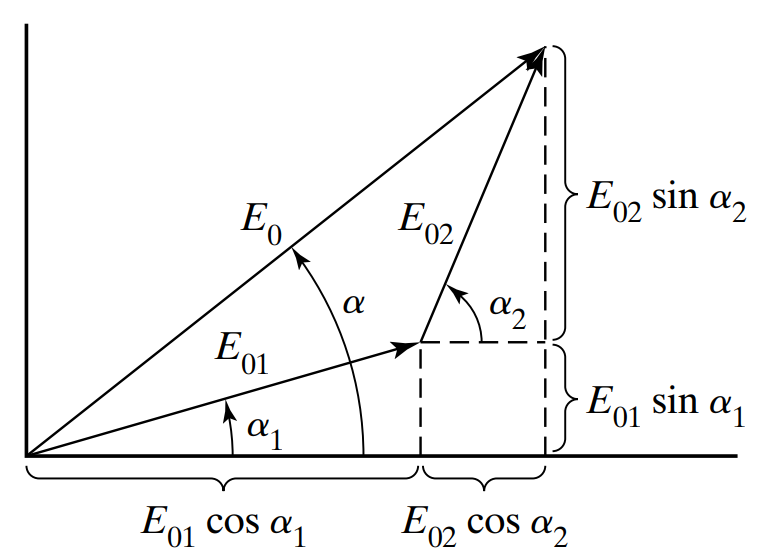
\includegraphics[scale=0.38]{superpo.png}
\end{center}
we can write the following:
\begin{align*}
E_0 \cos(\alpha) = E_{01}\cos(\alpha_1) + E_{02}\cos(\alpha_2) \qquad\qquad E_0\sin(\alpha) = E_{01} \sin(\alpha_1) + E_{02}\sin(\alpha_2)
\end{align*}
hence we get the following:
\begin{align*}
E_0^2 = E_{01}^2 + E_{02}^2 + 2E_{01}E_{02} \cos(\alpha_2 - \alpha_1)\qquad\qquad 
\tan(\alpha) = \frac{E_{01}\sin(\alpha_1) + E_{02}\sin(\alpha_2)}{E_{01}\cos(\alpha_1)+E_{02}\cos(\alpha_2)}
\end{align*}
We can extend this to superposition of many waves with the same frequency:
\begin{align*}
\tan(\alpha) = \frac{\sum_i E_{0i}\sin(\alpha_i)}{\sum_i E_{0i}\cos(\alpha_i)}
\end{align*}
\begin{align*}
E_0^2 =& \left( \sum_i E_{0i}\sin(\alpha_i)\right)^2 + \left( \sum_i E_{0i}\cos(\alpha_i)\right)^2\\
=&+ \sum_i E_{0i}^2 \sin^2(\alpha_i) + 2\sum_{j >1} \sum_i E_{0i}E_{0j}\sin(\alpha_j)\sin(\alpha_i) \\
 &+ \sum_i E_{0i}^2 \cos^2(\alpha_i) + 2\sum_{j >1} \sum_i E_{0i}E_{0j}\cos(\alpha_j)\cos(\alpha_i)\\
=&+ \sum_i E_{0i}^2 \left( \sin^2(\alpha_i) + \cos^2(\alpha_i) \right)\\
 &+ 2\sum_{j >1} \sum_i E_{0i}E_{0j}\left(\cos(\alpha_j)\cos(\alpha_i)+\sin(\alpha_j) + \sin(\alpha_i)\right)\\
=& \sum_{i} E_{0i}^2 + 2\sum_{j>1}\sum_i E_{0i}E_{0j}\cos(\alpha_j - \alpha_i)
\end{align*}
Now consider $N$ sources randomly phased, and of equal amplitude, then we have:
\begin{align*}
E_0^2 = \sum_{i=1}^N E_{0i}^2  = N E_{01}^2
\end{align*}
where the term $\cos(\alpha_j - \alpha_i)$ is minimized by the randomly phase property of the sources, and hence the irradiance of the superposition of the sources is just the sum of the individual sources.\\

Now consider instead we have $N$ coherent sources, then we can write:
\begin{align*}
E_0^2 = \sum_{i=1}^N E_{0i}^2 + 2\sum_{j>i}^N \sum_{i=1}^N E_{0i}E_{0j} = \left( \sum_{i=1}^N E_{0i}\right)^2 = (NE_{01})^2 = N^2 E_{01}^2
\end{align*}
the irradiance of $N$ coherent light is hence proportional to $N^2$. 

\subsection{Standing Waves}
We start by assuming that there is a perfect reflector, suppose wave is reflected and superposition with itself. The incoming wave and the reflected waves are given by the followings:
\begin{align*}
E_1 = E_0 \sin(\omega t+ kx) \qquad\qquad\qquad E_2 = E_0 \sin(\omega t- kx - \phi_k)
\end{align*}
where $\phi_k$ is phase shift due to reflection. Then the superposition of the two waves is given by the following:
\begin{align*}
E_R = E_1 + E_2 = E_0 \left( \sin( \omega t+ kx) + \sin(\omega t - kx - \phi_k)\right)
\end{align*}
We define the following phases:
\begin{align*}
\beta_+ = \omega t + kx \qquad\qquad\qquad \beta_- = \omega t -kx -\phi_k
\end{align*}
simple algebra yields:
\begin{align*}
E_R = 2E_0 \cos(kx + \phi_k/2) \sin(\omega t - \phi_k / 2)
\end{align*}
in the case where $\phi_k = \pi$ for metal mirror, we can write:
\begin{align*}
E_R = 2E_0 \sin(kx) \cos(\omega t) \tag{If $\phi_k = \pi$}
\end{align*}
For the \textbf{nodes} in standing wave, we have $E_R = 0$ at all $t$, which occurs at the positions $x$ given by the following:
\begin{align*}
kx = m\pi = \frac{2\pi}{\lambda}x \qquad\Rightarrow\qquad
x = \frac{m \lambda}{2} \qquad\qquad \forall m \in \N
\end{align*}
$E_R$ is at extremum for fixed position when we have $\cos(\omega t) = \pm 1$, or in other words:
\begin{align*}
\omega t = 2\pi \nu t = \frac{2\pi t}{T} = m \pi \qquad \forall m \in \N
\end{align*}
that is the outer envelope occurs for time $t = mT/2 = $ for $m\in \N$, and the wave is completely zero everywhere when $t = (2m-1)T/4$ for all $m \in \N$.\\

\subsection*{Laser Beam}
Laser light is generated in laser cavities, which often take the form of two
highly reflecting mirrors surrounding a gain medium. The light in such a cavity
then consists of counterpropagating electromagnetic waves that form standing
waves. If the distance between the cavity mirrors is $d$, the cavity will support standing waves with wavelengths $\lambda_m$ that satisfy:
\begin{align*}
d = m\frac{\lambda_m}{2} \qquad\qquad \forall	 m \in \N
\end{align*}
that is, we have:
\begin{align*}
\lambda_m = \frac{2d}{m}\qquad\qquad\forall  m\in \N
\end{align*}
the frequency of such beam is given by the following:
\begin{align*}
\nu_m = \frac{c}{\lambda_m} = \frac{mc}{2d}
\end{align*}

\example A He-Ne laser with $30\, cm$ mirror separation. The wavelength range from $\lambda_1 = 632.800\,nm$ to $\lambda_2 = 632.802\, nm$. The approximate number of half-wavelengths that fit the cavity is given by the following:
\begin{align*}
m = \frac{2d}{\lambda_1} \approx \frac{2\times 0.3\, m}{632.8\cdot 10^{-9}\, m} \approx 948166
\end{align*}
The range of frequencies supported by the medium is given by:
\begin{align*}
\Delta \nu = \frac{c}{\lambda_1}  - \frac{c}{\lambda_2} = 1.5\cdot 10^9 \, Hz
\end{align*}
The difference in frequencies in adjacent standing wave modes of the cavity is given by:
\begin{align*}
\nu_{m_1} - \nu_m = (m+1) \frac{c}{2d} -  \frac{mc}{2d} = \frac{c}{2d} = \frac{3\cdot 10^8\, m/s}{2\cdot 0.3\, m} = 5\cdot 10^{8}\, Hz
\end{align*}
The number of standing wave modes that will likely be present in the laser output is given by:
\begin{align*}
\frac{\Delta \nu }{\nu_{m+1} - \nu_m} = \frac{1.5\cdot 10^9 \, Hz}{5\cdot 10^8\, Hz} = 3
\end{align*}

\subsection{Different-frequency superposition}
Here we assume two waves with different frequencies in non-dispersive medium superimpose. Say the two incoming waves are modeled by the followings:
\begin{align*}
E_1 = \cos(k_1 x - \omega_1t) \qquad\qquad\qquad E_2 = \cos(k_2 x - \omega_2t)
\end{align*}
then the superposition of the two waves is given by the following:
\begin{align*}
E_R = E_1 + E_2 = E_0 \left( \cos(k_1 x - \omega_1 t) + \cos(k_2 x - \omega_2 t)\right)
\end{align*}
here we define:
\begin{align*}
\alpha = k_1 x - \omega_1 t \qquad\qquad\qquad \beta = k_2 x - \omega_2 t
\end{align*}
in which case we can write the following:
\begin{align*}
E_R = 2E_0 \cos\left( \frac{k_1 + k_2}{2}x - \frac{\omega_1 + \omega_2}{2}t\right) \cos\left( \frac{k_1 - k_2}{2}x - \frac{\omega_1 - \omega_2}{2}t\right)
\end{align*}
now define:
\begin{align*}
\omega_p = \frac{\omega_1 + \omega_2}{2} \qquad\quad \omega_g = \frac{\omega_1 - \omega_2}{2} \qquad\quad k_p = \frac{k_1+k_2}{2}\qquad\quad k_g = \frac{k_1 - k_2}{2}
\end{align*}
then combining we can write:
\begin{align}
E_R = \underbrace{2E_0 \cos(k_p x - \omega_p t)}_{\text{carrier}} \underbrace{\cos( k_g x - \omega_g t)}_{\text{envelope}}
\end{align}
The \textbf{beat frequency} is twice the frequency of the modulating envelop:
\begin{align*}
\omega_b = 2\omega_g = 2\left( \frac{\omega_1 - \omega_2}{2}\right) = \omega_1 - \omega_2
\end{align*}
In the case of sound, this is the usual beat frequency heard when two tuning forks are made to vibrate simultaneously, equal to the difference in fork frequencies. The phenomenon of beats provides a sensitive method of measuring the difference in frequencies of two signals of nearly the same frequency. Two guitarists may ensure that their guitars are in tune with each other by striking a note and listening for the beat note. One or the other of the guitarists may then adjust the tension in the guitar string until the beat note disappears, indicating that the guitars are in tune. In the optical arena, the beat phenomenon can be used to measure the difference between the emitted radar wave and the Doppler-shifted return signal in a Doppler weather radar system or as part of a feedback loop designed to ensure that two sources have the same
frequency. 




\subsection{Pulse and group velocity}
A pulse is a superposition of monochromatic waves, the duration of the pulse is usually inversely proportional to the range of the frequencies of the monochromatic waves. That is, narrower pulses are composed of harmonic waves with
a wider range of frequencies.\\

Electromagnetic waves at different frequencies have different speed due to dispersion of a medium. In dispersive media, the points of constructive interference will move at different speed from wave due to dispersion. The phase velocity of an electromagnetic signal is a measure of the velocity of the monochromative waves that constitute the signal, and the group velocity of the signal is the velocity at which the positions of the maximal constructive interference propagate. The velocity of the carrier wave characterized by (4.6) is given by the following:
\begin{align*}
v_p = \frac{\omega_p}{k_p} = \frac{\omega_1 + \omega_2}{k_1 + k_2} \approx \frac{\omega}{k}
\end{align*}
where we approximate that $\omega =\omega_1 \approx \omega_2$, and $k = k_1 \approx k_2$ for neighboring frequency and wavelength components in a continuum. The velocity of the envelop, called the group velocity, is given by the following:
\begin{align*}
v_g = \frac{\omega_g}{k_g} = \frac{\omega_1 - \omega_2}{k_1 - k_2} \approx \frac{d\omega}{dk}
\end{align*}
Note that we have the following relationship holds:
\begin{align*}
v_g = \frac{d\omega}{dk} = \frac{d}{dk}\left( k v_p\right) = v_p + k\left( \frac{dv_p}{dk}\right) = \frac{\omega}{k} + k\left( \frac{dv_p}{dk}\right)
\end{align*}
In a medium, we have $v_p = c/n$, with $n$ being a function of $k$. And hence we have:
\begin{align*}
\frac{dv_p}{dk} = \frac{d}{dk}\frac{c}{n} = -\frac{c}{n^2}\frac{dn}{dk} = -\frac{v_p}{n	} \frac{dn}{dk}
\end{align*}
combining we can write the following:
\begin{align*}
v_g = v_p \left( 1 - \frac{k}{n}\frac{dn}{dk}\right) = v_p \left( 1 + \frac{\lambda}{n}\frac{dn}{d\lambda}\right)
\end{align*}
In the regions of normal dispersion, we have $dn/d\lambda < 0$ and hence $v_g < v_p$. Hence we also see that, in non-dispersive medium, we have $v_g = v_p$. 



\newpage
\chapter{Interference of Light}
\section[Two-beam Interference]{\color{red} Two-beam Interference\color{black}}
Consider that we have two plane waves of the same frequency, we can write the followings for the two electric fields at a point $P$ where the fields superimpose:
\begin{align*}
\vec{E}_1 = \vec{E}_{01} \cos(ks_1 - \omega t + \phi_1) \qquad\qquad\vec{E}_{2} = \vec{E}_{02} \cos(ks_2 - \omega t + \phi_2)
\end{align*}
where we have $k = 2\pi / \lambda$, and the superposition of the two waves is given by:
\begin{align*}
\vec{E}_p  = \vec{E}_1 + \vec{E}_2
\end{align*}
and the irradiance of $\vec{E}$ is given by:
\begin{align*}
I = \epsilon_0 c \langle \vec{E}\cdot \vec{E}\rangle
\end{align*}
and hence at point $P$, we have:
\begin{align*}
I &= \epsilon_0 c \langle \vec{E}_p^2\rangle = \epsilon_0 c\langle(\vec{E}_1 + \vec{E}_2 ) \cdot (\vec{E}_1 + \vec{E}_2 ) \rangle\\
&= \epsilon_0 c \langle \, \underbrace{\vec{E}_1 \cdot \vec{E}_1 + \vec{E}_2 \cdot \vec{E}_2}_{\substack{\text{irrandiance of}\\ \text{individual beams}}} \,+ \underbrace{2\vec{E}_1 \cdot \vec{E}_2}_{\substack{\text{irradiance of} \\\text{ interference}}} \rangle
\end{align*}
In which case we see that we can write:
\begin{align*}
I = I_1 + I_2 + I_{12}
\end{align*}
where we define:
\begin{align*}
I_{12} = 2\epsilon_0 c \langle \vec{E}_1 \cdot \vec{E}_2\rangle =  2\epsilon_0 c  \left(\vec{E}_{01}\cdot \vec{E}_{02}\right) \langle\cos(ks_1 -\omega t + \phi_1)\cos(ks_2 - \omega t +\phi_2)\rangle
\end{align*}
Here we define:
\begin{align*}
\alpha = ks_1 + \phi_1\qquad\qquad\qquad \beta = ks_2 + \phi_2
\end{align*}
then we can write the following:
\begin{align*}
2\langle\vec{E}_{1}\cdot \vec{E}_{2}\rangle 
&= 2\left(\vec{E}_{01}\cdot \vec{E}{02}\right) \langle\cos(\alpha - \omega t) \cos(\beta - \omega t)\rangle\\
&= 2\left(\vec{E}_{01}\cdot \vec{E}{02}\right) \left( \langle \cos(\alpha+\beta - 2\omega t)\rangle + \langle \cos(\beta - \alpha) \rangle\right)
\end{align*}
where the term $\langle \cos(\alpha+\beta - 2\omega t)\rangle = 0$ because of the time average of rapidly varying cosine function, hence now we obtain:
\begin{align*}
2\langle\vec{E}_1 \cdot \vec{E}_2\rangle &= 
\left(\vec{E}_{01}\cdot \vec{E}_{02}\right) \langle \cos(\beta - \alpha)\rangle\\
&= \left(\vec{E}_{01}\cdot \vec{E}_{02}\right)\langle \cos(k(s_2 - s_1) + \phi_2 - \phi_1)\rangle\\
&= \left(\vec{E}_{01}\cdot \vec{E}_{02}\right)\langle \cos(\delta)\rangle
\end{align*}
where we define: 
\begin{align}
\delta = k(s_2-s_1)+\phi_2 - \phi_1
\end{align}
For monochromatic field, $\delta$ is time independent, and hence $\langle \cos(\delta) \rangle = \cos(\delta)$.\\
Now combining, we can write the following:
\begin{align*}
I_R = \epsilon_0 c \left( \vec{E}_{01}\cdot \vec{E}_{02}\right) \langle \cos(\delta) \rangle
\end{align*}

In particular, we have:
\begin{align*}
I_1 = \langle \vec{E}_1 \cdot \vec{E}_1 \rangle = \epsilon_0 c \vec{E}_{01}\langle \cos^2(\alpha - \omega t)\rangle  = \frac{1}{2}\epsilon_0 c E_{01}^2\qquad\qquad I_2 = \frac{1}{2}\epsilon_0 c E_{02}^2
\end{align*}

Hence we have:
\begin{align*}
I_{12} = 2\sqrt{I_1I_2}\langle\cos(\delta) \rangle
\end{align*}
In which case we can write:
\begin{align}
I = I_1 + I_2 + 2\sqrt{I_1I_2}\langle \cos(\delta) \rangle
\end{align}
For mutually incoherent beam, one can approximate that we have $\langle \cos(\delta) \rangle$ approaches zero, and hence we have the following irradiance for incoherent beam:
\begin{align*}
I = I_1 + I_2 \tag{incoherent beam}
\end{align*}
For mutually coherent beam, such a two copies of a single laser, we then have $\phi_1(t) - \phi_2(t) = 0$ if the beams travel paths of equal duration before being recombined at the detector. In which case we can write:
\begin{align*}
I = I_1+I_2+ 2\sqrt{I_1I_2} \cos(k(s_2 - s_1)) \tag{coherent beam}
\end{align*}
If there is a time delay $\delta t$ between the two beams, that is $\phi_1(t) - \phi_2(t) = \phi_1(t) - \phi_1(t+\delta t) $, we get nearly the same results for $I_{12}$ as long as $\delta t$ is smaller than the coherent time $\tau_0$. The coherence time of the source is the time interval over which departures from monochromaticity are small, and is inversely proportional to the range of frequencies $\Delta \nu$ of the beam:
\begin{align*}
\tau_0 = \frac{1}{\Delta \nu}
\end{align*}
Similarly we have the coherence length defined by $l_t = c\tau_0$, which is the distance that the electric field travels in a coherence time. For a white
light source the coherence length is about $1\mu m$. Laser sources have coherence lengths that range from tens of centimeters to tens of kilometers.\\

For coherent beam, now we assume $\Delta l < l_t$. $\delta = k(s_2 - s_1)$ is a phase difference due to path length difference of the beams, the path difference can be due to reflection phase shift, and the index of refraction of a media. If $\cos(\delta) = 1$, in which case $\delta = 2\pi m$ for some $m\in \Z$, then we obtain the maximum irradiance:
\begin{align*}
I_{max} = I_1 + I_2 + 2\sqrt{I_1 I_2}
\end{align*}
and if $\cos(\delta) = -1$, in which case $\delta = (2m+1)\pi $ for some $m\in \Z$,  we obtain the minimum irradiance:
\begin{align*}
I_{min} = I_1 + I_2 - 2\sqrt{I_1 I_2}
\end{align*}
Typically, $\cos(\delta)$ will take on alternating maximum and minimum values, and interference fringes, spatially separated, will occur in the observation plane. The fringe constant, or the visibility of such interference pattern, is defined by the following:
\begin{align*}
\text{visibility} = \frac{I_{max} - I_{min}}{I_{max} + I_{min}}
\end{align*}
For balanced beam, that is if we have $I_1 = I_2 = I_0$, then we can write:
\begin{align}
I = I_0 + I_0 = 2\sqrt{I_0^2}\cos(\delta) = 2I_0(1+ \cos(\delta)) = 4I_0 \cos^2(\delta /2)
\end{align}
\example Suppose we have:
\begin{align*}
I_1 &= \frac{1}{2}\epsilon_0 c E_{01}^2 = \frac{1}{2}\epsilon_0 c\left( 2000\right)^2 = 5309\, W/m^2\\
I_2 &= \frac{1}{2}\epsilon_0 c E_{02}^2 = \frac{1}{2}\epsilon_0 c(5000)^2 = 33180 \, W/m^2
\end{align*}
and suppose we have $k(s_2 - s_1) = \pi/12$, then we have:
\begin{align*}
I_{12} =2\sqrt{I_1 I_2}\cos(\delta) = \sqrt{5309 \cdot 33180}\cos(\pi/12) = 25640\, W/m^2
\end{align*}
To find the visibility:
\begin{align*}
I_{max} &= I_1 + I_2 + 2\sqrt{I_1I_2} = 5309 + 33180 + 2\sqrt{5309 \cdot 33180} = 65034\, W/m^2\\
I_{min} &=  I_1 + I_2 - 2\sqrt{I_1I_2} = 5309 + 33180 - 2\sqrt{5309 \cdot 33180} =11945\, W/m^2
\end{align*}
and hence the visibility:
\begin{align*}
\text{visibility} = \frac{65034 - 11945}{65034 + 11945} = 0.69
\end{align*}

\newpage
\section[Double-slit Interference]{\color{red}Double-slit Interference\color{black}}
A monochromatic light beam is first allowed to pass through a single small hole in order to approximate a single point source $S$. The light spreads out in spherical waves from the source $S$ according to Huygens' principle and is allowed to fall on a plane with two closely spaced holes, and the holes become two coherent sources of light, whose interference can be observed on a screen some distance away. If the two holes are equal in size, light waves emanating from the holes have comparable amplitudes, and the irradiance at any point of superposition is given by (5.3). Referring to the following geometry, we will now develop an expression for the irradiance at observation points such as $P$ on a screen that is a distance $L$ from the plane containing the two holes.
\begin{center}
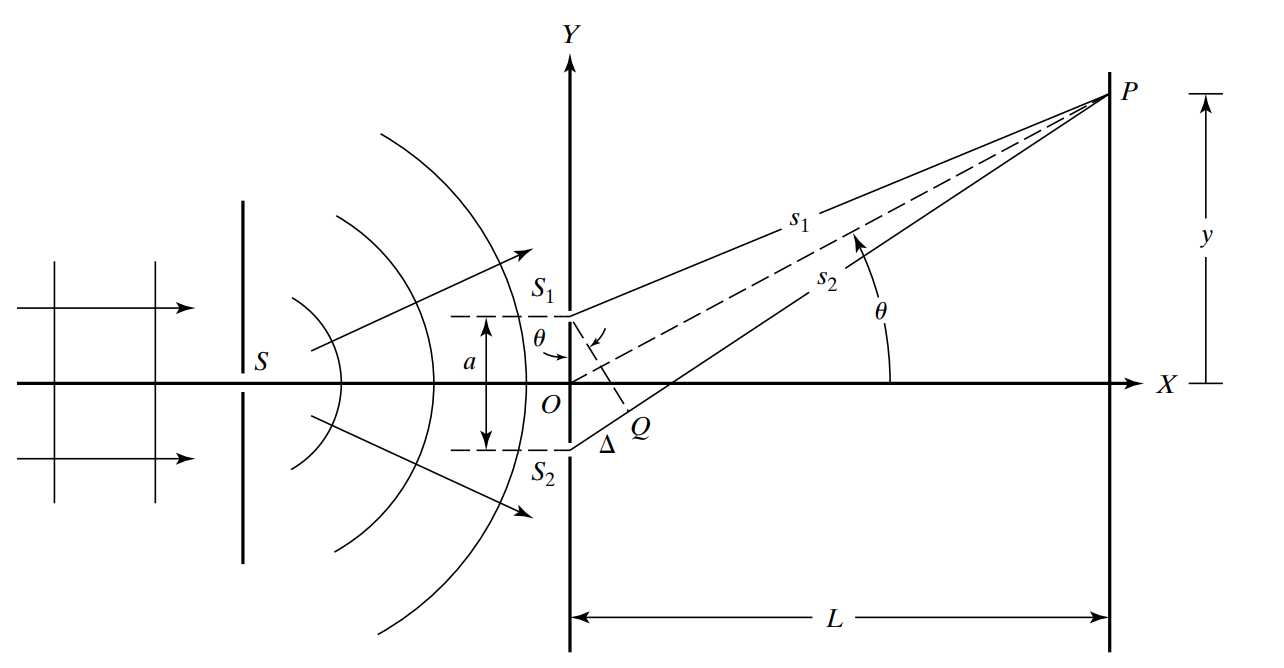
\includegraphics[scale=0.45]{doubleSlit.png}
\end{center}
Here we assume that the beams from $S_1$ and $S_2$ are coherent. If we have $S_2P - S_1 P = s_2 - s_1 = m\lambda$, then the waves are in phase, and hence we get bright fringes. In instead we have $s_2 - s_1 = (m+1/2) \lambda$, then the waves are out of phase, and hence we get dark fringes. For approximation $a<<L$, we can write $s_2 - s_1 = \Delta$, and we can approximate $\Delta = a\sin(\theta)$. For constructive interference, we then write:
\begin{align*}
s_2 -s_1 = \Delta  = m \lambda  = a\sin(\theta)
\end{align*}
For destructive interference, we then write:
\begin{align*}
s_2 - s_1 =\Delta  = (m+1/2) \lambda = a\sin(\theta)
\end{align*}
where $m \in \Z$. In such case, the angular difference in path $\delta$ of the two coherent waves is given by the following:
\begin{align*}
\delta = k(s_2 - s_1) \frac{2\pi }{\lambda}\Delta
\end{align*}
Hence we can write the irradiance of the fringes:
\begin{align*}
I = 4I_0 \cos^2\left( \frac{\pi \Delta}{\lambda}\right) = 4I_0 \cos^2\left(\frac{\pi a \sin(\theta)}{\lambda}\right)
\end{align*}
One can assume that we have $y<<L$, then we have $\sin(\theta) \approx \tan(\theta) \approx y/L$, that is, bright fringes occurs at positions $y_m$ from the axis $X$ given by the following:
\begin{align*}
y_m  = \frac{m\lambda L}{a} \qquad m\in \Z
\end{align*}
and the spacing between fringes is given by:
\begin{align*}
\Delta y = y_{m+1}-y_m = \frac{\lambda L}{a}
\end{align*}


\newpage
\section[Dielectric Films]{\color{red}Dielectric Films\color{black}}
Interference occurs due to optical path length difference when light goes through a thin coat of dielectric material of refraction index $n_f$. Suppose the light goes from material with refraction index $n_0$, after passing through the film, the light hits the substrate which has refraction index $n_s$. \\
\begin{center}
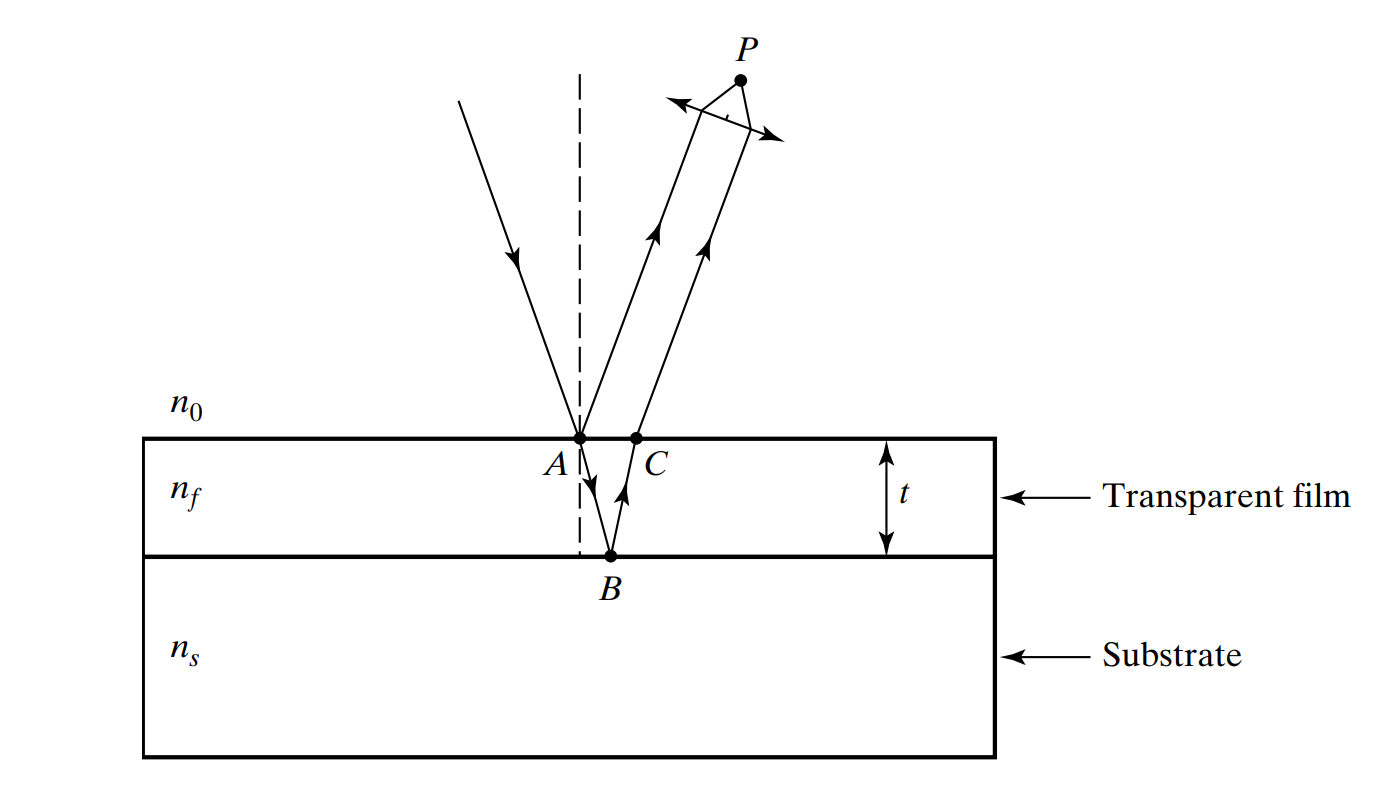
\includegraphics[scale=0.39]{film.png}
\end{center}
For normal incidence, let $t$ denote the thickness of the film, then the path difference between the reflected light and the refracted-reflected-refracted light is given by the following:
\begin{align*}
\Delta_p = n(AB+BC) = n(2t)
\end{align*}
Here we only account for optical path difference, one also need to consider the phase shift on reflection $\Delta_s$. Consider that we have $n_f > n_0$ and $n_f > n_s$, then reflection at $A$ is said to be external, and the reflection at $B$ is said to be internal. The reflective phase shift between internal and external is given by $\pi$, leads to a difference in path given by $\Delta_s = \lambda_0/ 2$. When we have $\Delta_s+ \Delta_p = m\lambda_0$, which is $m$ times the wavelength of the incident light, then we have constructive interference at point $P$.\\

Consider normal incident light of wavelength $\lambda_0$. For usual case, we consider $n_0 = 1$ and $n_f > n_0$. If we have $n_s > n_f$, then there is no phase shift due to reflection $\Delta_s$. If the thickness $t=\lambda_f/4$, where $\lambda_f$ is the wavelength of the light in the transparent film, then we have $2t = \lambda_f / 2$, and so:
\begin{align*}
\Delta_p= 2n_ft = \frac{\lambda_0}{2}
\end{align*}
getting constructive interference with the reflected incoming light. Note that this is for only one specific wavelength, for nearby wavelengths, the destructive interference is not perfect. We also require equal amplitude for perfect destructive interference. \\

One can compute that the reflection coefficient is given by:
\begin{align*}
r = \frac{1-n}{1+n} \qquad\qquad n=\frac{n_2}{n_1}
\end{align*}
where $n_1$ is the refraction index of the material for incident light, and $n_2$ is the refraction index of the material at which the incident light is reflected. $r$ is sufficiently low in most cases, and hence transmission rate is comparable to $1$. As a result, one can compute the condition where the amplitude of the two reflected waves are equal:
\begin{align*}
\frac{n_f}{n_0} = \frac{n_s}{n_f} \qquad \Rightarrow \qquad n_f =\sqrt{n_0 n_s}
\end{align*}
In the limit $n_0 = 1$, we want $n_f = \sqrt{n_s}$. \\

Now suppose the incident light is not at normal to the boundary, as in the geometry:
\begin{center}
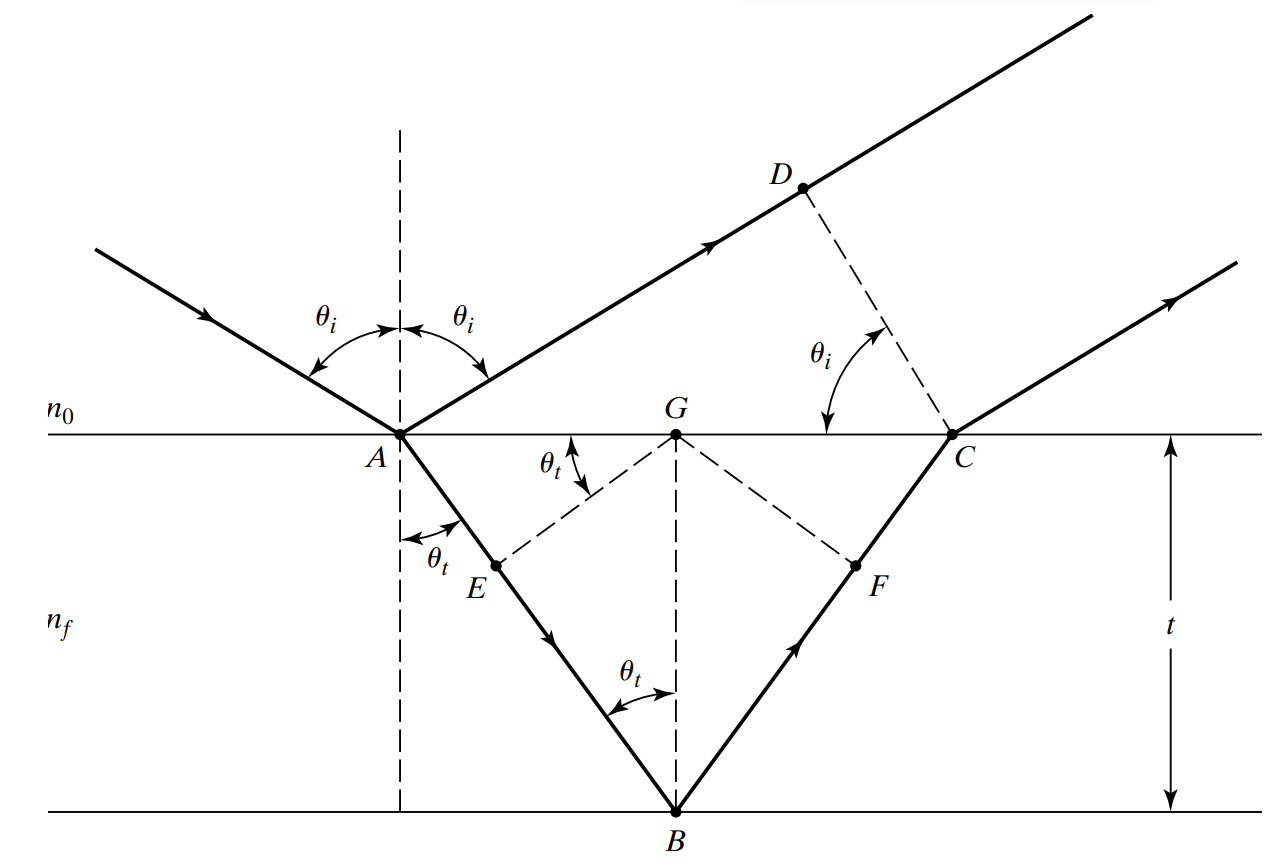
\includegraphics[scale=0.45]{tiltedFilm.png}
\end{center}
Here we can write:
\begin{align*}
\Delta_p &= n_f(AB+BC)-n_0 AD \\
&= \left( n_f(AE+FC) -n_0 AD\right) + n_f(EB+BF)
\end{align*}
where we have:
\begin{align*}
n_o \sin(\theta_t) = n_f \sin(\theta_i) \qquad\qquad\qquad
AE &= AG \sin(\theta_t) = AC/2 \, \sin(\theta_t)\\
AD &= AC \sin(\theta_i)
\end{align*}
combining we obtain:
\begin{align*}
2AE &= AC\sin(\theta_t) = AD (\sin(\theta_t) / \sin(\theta_i)) =AD (n_0 / n_f)
\end{align*}
so we get:
$$
n_0 AD = 2n_f AE = n_f(AE+FC)$$
Now we have: 
$$\Delta_p = n_f(EB+BF) = 2n_f EB = 2n_f t\cos(\theta_t)$$
For normal incidence $\theta_i = \theta_t = 0$, and hence $\Delta = 2n_f t$ as expected. \\
The corresponding phase difference due to difference in path is given by the following:
\begin{align*}
\delta_p = k\Delta_p = \frac{2\pi}{\lambda_0}\Delta_p
\end{align*}
note that the phase shift due to reflection $\Delta_r$ should also be considered when computing conditions for constructive or destructive interference. \\

We have constructive interference if we have $\Delta_p + \Delta_r = m\lambda$, and destructive interference if we have $\Delta_p + \Delta_r = (m+1/2) \lambda$. Fringes produced by a lines source with a film of equal or varying thickness are called the Fizeau fringes. The condition for bright and dark fringes is given by:
\begin{align*}
2n_f t +\Delta_r = \begin{cases} m\lambda & \text{bright fringe}\\
(m+1/2) \lambda) & \text{dark fringe}
\end{cases}
\end{align*}
where the optical path difference $\Delta_p = 2n_f t\cos(\theta_t)$ varies regardless of the variation in the angle of incidence. \\

An important application is the Newton's Ring.  An air wedge, formed between the spherical surface and an optically flat surface, is illuminated with normally incident monochromatic light. Circular fringes are seen on the screen above the spherical surface. If the spherical surface is not perfectly circular, the circular fringes will be distorted. 
\begin{center}
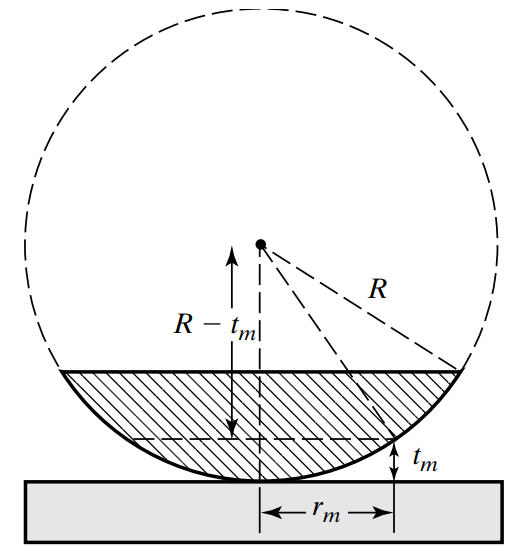
\includegraphics[scale=0.55]{newton.png}
\end{center}
where we have dark fringe at the center. The radius of curvature $R$ of the air film, or the lens surface, by geometry, can be determined via the following:
\begin{align*}
R^2 = r_m^2 + (R-t_m)^2 \qquad\Rightarrow \qquad R = \frac{r_m^2 + t_m^2}{2t_m}
\end{align*}

\hfill\break

\example
A plano-convex lens of $1/8$ diopter power is placed, convex surface down, on an optically flat surface. Using a traveling microscope and sodium light $\lambda = 589.3\, nm$ interference fringes are
observed. Determine the radii of the first and tenth dark rings.\\

In this problem we have $\Delta_r = \lambda/2$, hence the thickness at the $m^{th}$dark ring is given by $t_m = m\lambda / (2n_f) = m\lambda / 2$ where $n_f = 1$ for air film. The ring radii are then given by:
\begin{align*}
R^2 = r_m^2 + ( R - t_m)^2 \qquad \Rightarrow \qquad r_m^2 = 2t_m R - t_m^2
\end{align*}
the term $t_m^2$ is small compared to $R$, hence to be neglected. \\
Now we apply the lensmaker's formula:
\begin{align*}
\frac{1}{f} = (n-1) \left( \frac{1}{R_1} - \frac{1}{R_2}\right)
\end{align*}
where $f = 8\, m$, $n=1.523$, and $R_2 = \infty$, that gives $R_1 = R = 4.184$. Hence we have:
\begin{align*}
r_m^2 = 2Rt_m = 2R \left( \frac{m\lambda}{2}\right) = mR\lambda
\end{align*}
so $r_1^2 \approx 2.466\cdot 10^{-6}\, m^2$, and $r_{10}\approx 24.66 \cdot 10^{-6}\, m^2$.

\newpage
\section[Stokes Relations]{\color{red}Stokes Relations\color{black}}
Let $E_i$ represent the amplitude of the incident light, $E_r, E_t$ be the amplitudes of the reflected and transmitted light, we define the reflection and transmission coefficients by the following:
\begin{align*}
r = \frac{E_r}{E_i} \qquad\qquad\qquad t = \frac{E_t}{E_i}
\end{align*}
Note that $E_i$ in the first region is divided into a reflected part $E_r = rE_i$ in the first region and a transmitted part $E_t = tE_i$ in the second region. For a light that goes from the second region to the first region, we denote the reflection and transmission coefficients as $r'$ and $t'$. While according to the principle of ray reversibility, the original transmitted ray, when direction is reversed, also has reflected portion in the second region, and the transmitted part back to the first region. As shown in the following geometry:
\begin{center}
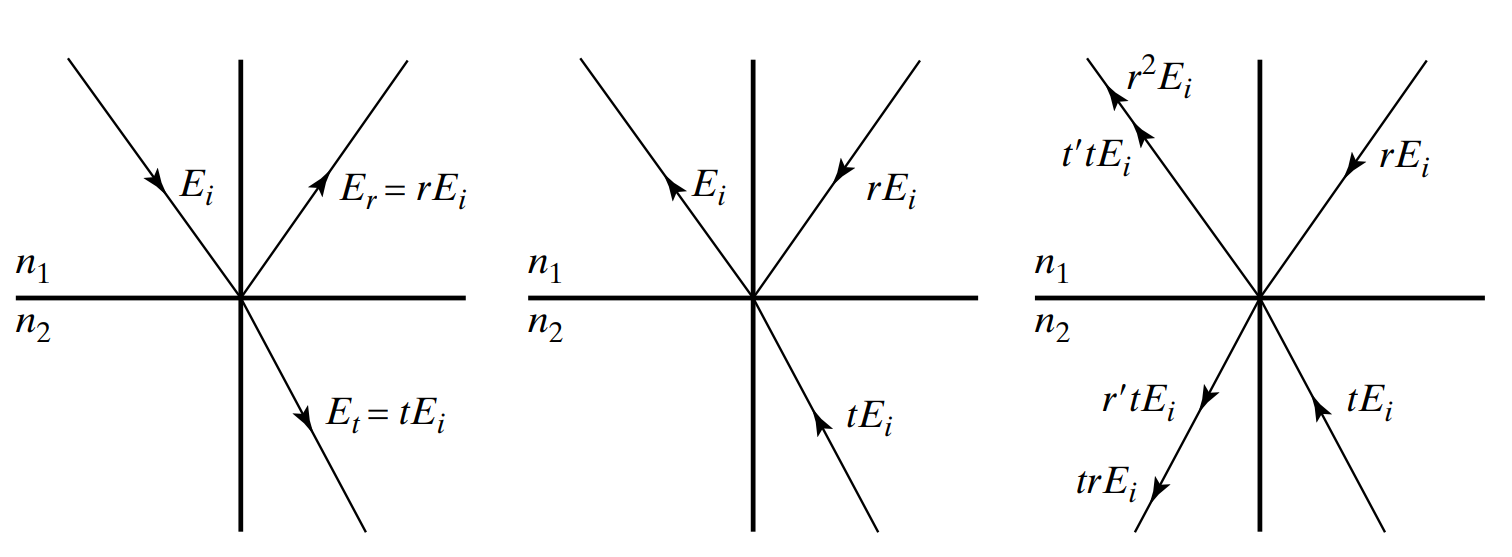
\includegraphics[scale=0.39]{stokes.png}
\end{center}
The two situations, before and after reversing the light, must be equivalent, that is we require the following holds:
\begin{align*}
E_i = (r^2 + t't) E_i \qquad\qquad\qquad 0 = (r't+tr)E_i
\end{align*}
that is, we obtain the Stokes relations:
\begin{align*}
tt' = 1-r^2 \qquad \qquad \qquad r= -r'
\end{align*}

\newpage
\section[Multibeam Interference]{\color{red}Multibeam Interference\color{black}}
Consider a place of some thickness $t$, and has index of refraction $n_f$. An incident beam has amplitude $E_0$ and incident the plate at an angle $\theta_i$. From air to the plate, denote the transmission and reflection coefficients as $t,r$. From plate to air, denote the transmission and reflection coefficients as $t',r'$. 
\begin{center}
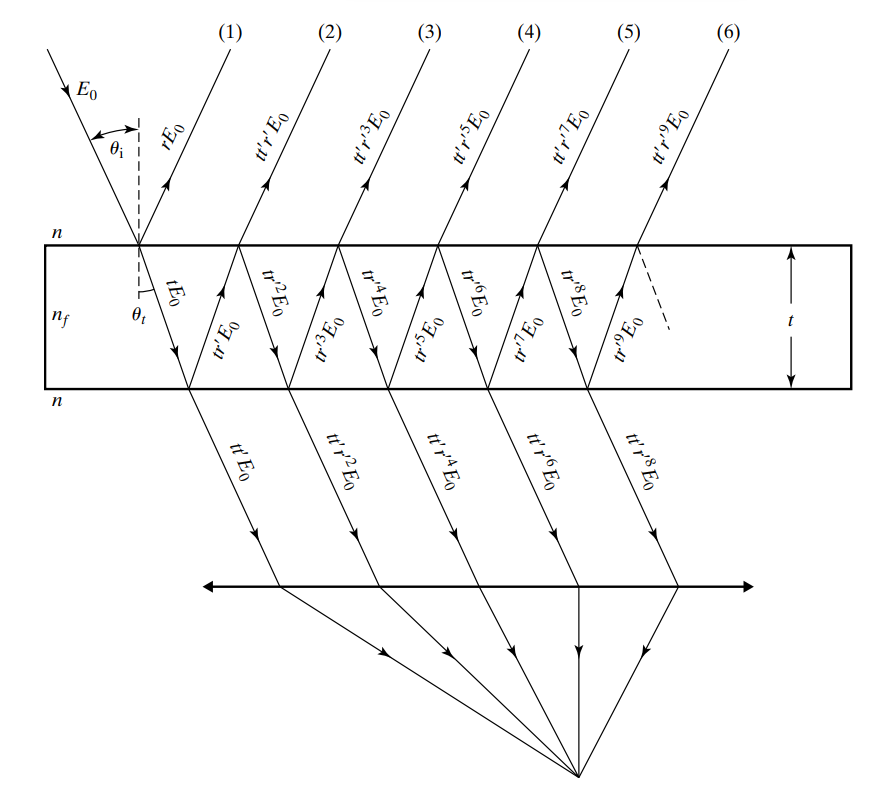
\includegraphics[scale=0.80]{multiFilm.png}
\end{center}
Consider the phase difference between successive reflected beams is given by $\delta = k \Delta$, where $\Delta = 2n_f t \cos(\theta_t)$. If the incident wave is characterized by $E_0 e^{i\omega t}$, then we can write the following with $N\geq 2$ for field of the $N$-th reflected wave:
\begin{align*}
E_1 = (rE_0)e^{i\omega t} \qquad\qquad\qquad E_N = (tt'{r'}^{(2N-3)}E_0) e^{i(\omega t - (N-1)\delta)}
\end{align*}
When the waves are superposed, the resultant $E_R$ may be written as the following by employing geometric series and Stokes relations:
\begin{align*}
E_R = \sum_{N=1}^\infty E_N &= rE_0 e^{i\omega t} + \sum_{N=2}^\infty tt'E_0 {r'}^{(2N-3)}e^{i(\omega t - (N-1)\delta}\\
&= E_0 e^{i\omega t}\left( r + tt'r'e^{-i\delta}\sum_{N=2}^\infty {r'}^{(2N-4)} e^{-i(N-2) \delta}\right) \\
&= E_0 e^{i\omega t}\left( r + \frac{tt'{r'}e^{i\delta}}{1-{r'}^2e^{-i\delta}}\right)\\
&= E_0 e^{i\omega t}\left( r - \frac{(1-r^2) re^{-i\delta}}{1-r^2 e^{-i \delta}}\right)\\
&= E_0 e^{i\omega t}\left( \frac{r(1-e^{-i\delta})}{1-r^2 e^{-i\delta}}\right)
\end{align*}
Now here the irradiance $I_R$ of the resultant beam is proportional to the square of the amplitude $E_R$, which is itself complex, so $I_R = |E_R|^2$:
\begin{align*}
|E_R|^2 = E_0^2 r^2 \left(\frac{e^{i\omega t}(1-e^{-i\delta}}{1-r^2 e^{-i\delta}} \right)\left( \frac{e^{-i\omega t}(1-e^{i\delta})}{1-r^2 e^{i\delta}}\right)= 2E_0^2r^2 \left( \frac{1-\cos(\delta)}{1+r^4-2r^2 \cos(\delta)}\right)
\end{align*}
concluding we see that we have:
\begin{align*}
I_R = \left( \frac{2r^2 (1-\cos(\delta))}{1+r^4 - 2r^2 \cos(\delta)}\right) I_i
\end{align*}
where $I_i$ represents the irradiance of the incident beam. A similar treatment of the transmitted beams leads to the resultant transmitted irradiance:
\begin{align*}
I_T = \left( \frac{(1-r^2)^2}{1+r^4 - 2r^2 \cos(\delta)}\right)I_i
\end{align*}
Note here we must have $I_R + I_T = I_i$, as required by the conservation of energy for nonabsorbing films.\\

The minimum in the reflected irradiance occurs when we have $\cos(\delta) = 1$, or when we have the following for some $m\in \Z$:
\begin{align}
\delta = 2\pi m \qquad \Rightarrow\qquad \Delta = 2n_f t\cos(\theta_t) = m\lambda
\end{align}
and (5.4) here also gives the transmission maximum. In such situation characterized by (5.4), one can argue that $E_1$ is canceled exactly by the sum of $E_N$ with $N \geq 2$. That is, at reflection minimum, the first reflected beam is $\pi$ out-of-phase with the rest of the reflected beam. The two-analysis works when we have $E_2 \approx E_1$, note here we can compute:
\begin{align*}
\left|\frac{E_2}{E_1}\right| = \left|\frac{tt'r'E_0}{rE_0}\right| = 1-r^2
\end{align*}
which is approximately $1$ when $r$ is small enough. At normal incidence, on glass of $n=1.5$ and $r^2 = 0.04$, around $96\%$ of the cancellation occurs between the first two reflected beams alone. \\

For reflection maximum, occurs when $\cos(\delta) = -1$, that is, we require:
\begin{align*}
\delta = (m+1/2)2\pi \qquad \Rightarrow \qquad \Delta = 2n_f t \cos(\theta_t) = (m+1/2) \lambda
\end{align*}
In this case, one can compute that we have:
\begin{align*}
I_R = \left( \frac{4r^2}{(1+r^2)^2}\right)I_i \qquad\qquad \qquad I_T = \left( \frac{1-r^2}{1+r^2}\right)^2 I_i
\end{align*}

\newpage
\chapter{Interferometer}
An interferometer is a device that exploit interference of light. There are ways to divide the light. One way is through wavefront division, which was used in the Young's double-slit experiment. Another way is through amplitude division, which is employed by beam splitter in the Michelson interferometer. The Michelson interferometer uses two splitted beams to form interference patter, while Fabry-Perot interferometer uses many splitted beams. 
\section[Michelson Interferometer]{\color{red}Michelson Interferometer\color{black}}
From an extended source of light S, beam 1 of light is split by a beam splitter
(BS). Reflected beam 2 and transmitted beam 3, of roughly equal amplitudes, continue to fully-reflecting mirrors M2 and M1, respectively, where their directions are reversed. On returning to the beam splitter, beam 2 is now transmitted and beam 3 is reflected by the semitransparent film so that they come together again and leave the interferometer as beam 4. The useful aperture of this double-beam interferometer is such that all rays striking M1 and M2 will be normal, or nearly so. Thus, beam 4 includes rays that have traveled different optical paths and will demonstrate interference. Note here the following two systems are equivalent when regarding S' as the source S in the interferometer and M1' as M1 in the interfereometer. 
\begin{center}
\includegraphics[scale=0.55]{Michelson.png}
\end{center}
The path difference between beam 2 and beam 3 is then given by the following:
\begin{align*}
\Delta_p = 2d\cos(\theta) \qquad \Rightarrow \qquad \Delta_p = 2d \text{ when }\theta = 0
\end{align*}
If $\Delta_p = m\lambda$, we see constructive interference, in which case we require $d = m \lambda /2$ in the case where $\theta = 0$. This behavior repeats for every $\lambda/2$ within coherence length. For fixed $d$, we get circular fringes, where we have:
\begin{align*}
I = 4I_0 \cos^2(\delta/2) \qquad \qquad \qquad \delta = k\Delta = \frac{2\pi}{\lambda}\Delta
\end{align*}
and here $\Delta = \Delta_p + \Delta_r$, where $\Delta_r = \lambda/2$. For dark fringe, here we require: 
\begin{align}
\Delta_p +\Delta_r = 2d\cos(\theta)+\lambda/2 = (m+1/2)\lambda \qquad \qquad \qquad 2d\cos(\theta) = m\lambda
\end{align}
If a fixed $d$ is such that normal rays satisfy $2d = m\lambda$, then the center is dark, and hence we can define $m_{max}$ to be the following:
\begin{align*}
m_{max} = \frac{2d}{\lambda}
\end{align*}
neighboring fringes decrease in order going out as $\cos(\theta)$ decreases from $1$:
\begin{align*}
p = m_{max} - m = \frac{2d}{\lambda} - m = \frac{2d}{\lambda } -m
\end{align*}
rearranging we get the condition for dark fringe:
\begin{align}
p\lambda = 2d(1-\cos(\theta))
\end{align}
for $p \in \N\cup\{0\}$. here now the central fringe is of order zero and the neighboring fringes increase in order, outward from the center. From (6.2), as $d$ changes, $p$ should also change to maintain a fixed $\theta$. Integer values for $p$ occur whenever the point in the center of the fringe coincides with a dark fringe. Equivalently, this means that as d is varied, fringes of the pattern appear to move inward toward the center, where they disappear, or else move outward from the center, where they seem to originate, depending on whether the optical-path difference is decreasing or increasing. The motion of the fringe pattern thus reverses as one of the mirrors is moved continually through the point of zero path difference. \\

Moreover, from (6.1), there is an increase in angular separation $\Delta \theta$ of a given small fringe interval $\Delta m$ as the mirror spacing $d$ becomes smaller, that is:
\begin{align*}
\left|\frac{d\theta}{dm}\right| = \frac{\lambda}{2d\sin(\theta)}
\end{align*}
This means that the fringes are more widely separated when optical-path differences are small. For a mirror translation $\Delta d$, the number $\Delta m$ of fringes passing a point at or near the center of the pattern is given by:
\begin{align*}
\Delta m = \frac{2\Delta d}{\lambda}
\end{align*}
which gives us a way to measure $\lambda$ experimentally. \\

If one has two sources of nearby wavelengths $\lambda, \lambda'$. The fringe pattern will coincide if we have $m\lambda = m'\lambda'$ at some $d_1$ according to (6.1), and at this point, we denote the order $m' = m-N$. If one changes $d$, the fringe will first be washed out, and if one changes $d$ furhter to $d_2$ at which the patterns coincide again, then we can write, we have $m\lambda = m'\lambda$ again but at this point we have $m' = m-(N+1)$. Combing using equation (6.1), we can write:
\begin{align*}
\frac{2d_1}{\lambda} = \frac{2d_1}{\lambda'} + N \qquad\qquad\qquad \frac{2d_2}{\lambda} = \frac{2d_2}{\lambda'}+(N+1)
\end{align*} 
From here, we can calculate the difference in wavelengths:
\begin{align*}
\lambda' - \lambda = \frac{\lambda\lambda'}{2\Delta d} \approx \frac{\lambda^2}{2\Delta d}
\end{align*}

\newpage
\section[Fabry-Perot Interferometer]{\color{red} Fabry-Perot Interferometer\color{black}}
The Fabry-Perot interferometer makes use of an arrangement similar to the
plane parallel plate to produce an interference pattern that results from the superposition of the multiple beams of the transmitted light.
\begin{center}
\includegraphics[scale=0.55]{fbCavity.png}
\end{center}


The glass plates function as mirrors and the arrangement is often called a \textbf{cavity}. The condition that characterizes bright fringe is given by:
\begin{align*}
2d \cos(\theta_t) = m\lambda
\end{align*}
Hence for fixed $d$, the interference pattern is concentric rings, as illustrated in Figure (a). Another configuration is one can place photodetector at one end, and that records intensity as a function of plate spacing $d$, as illustrated in Figure (b).
\begin{center}
\includegraphics[scale=0.65]{ab}
\end{center}

Assuming that both mirror 1 and mirror 2 have transmission and reflection coefficient $t,r$. Denote the the incoming wave, as it hits mirror 1, as $E_I$, denote the reflected wave as $E_R$, denote the right-going wave between the mirrors, at the position of mirror 1, at the time when incoming wave hits mirror 1, as $E_1^+$, denote the wave that is transmitted through mirror 2 as $E_T$. Here we obtain the followings:
\begin{align*}
r^2 + t^2 = 1
\end{align*}
\begin{center}
\includegraphics[scale=0.55]{fbTrans.png}
\end{center}
The \textbf{cavity round-trip time} is the time needed for light to circulate once around the cavity, given by:
\begin{align*}
\tau = \frac{2d}{v} = \frac{2nd}{c}
\end{align*}
Here we define the propagation factor $P_F(\Delta z, \Delta t)$ to be the ratio of the field, as a complex quantity, associated with a traveling monochromatic plane wave at position $z = z_0 + \Delta z$ and at time $t = t_0 +\Delta t$ to the same field at position $z = z_0$ and at time $t = t_0$, that is:
\begin{align*}
E(z_0 + \Delta z, t_0+\Delta t) = P_F(\Delta z, \Delta t) \, E(z_0 ,t_0)
\end{align*}
Hence we get:
\begin{align}
P_F(\Delta z, \Delta t) = \frac{E(z_0 + \Delta z , t_0 + \Delta t)}{E(z_0, t_0)} = \frac{E_0 e^{i( \omega (t_0 + \Delta t) - k(z_0 + \Delta z))}}{E_0 e^{i(\omega t_0 - kz_0)}} = e^{i (\omega \Delta t - k\Delta z)}
\end{align}
Here we assume that we have:
\begin{align*}
E_I = E_{0I}e^{i\omega t} \qquad\qquad\qquad E_1^+ = E_{01}^+ e^{i\omega t}
\end{align*}
note here $E_{0I}$ is a constant while $E_{01}^+$ depends on $t$, hence we denote $E_{01}^+(t)$. At time $t + \tau$, we can write:
\begin{align*}
E_1^{+}(t+\tau) = tE_I(t+\tau) + r^2 P_F(2d, \tau) E_1^+(t)
\end{align*}
combining with (6.3) we get the following:
\begin{align}
E_{01}^+(t+\tau)e^{i\omega (t+\tau)} = t E_{0I}e^{i\omega(t+\tau)} + r^2 E_{01}^+(t)e^{i\omega t}e^{i(\omega \tau -2kd)}
\end{align}
Once we reach a steady state, we must have $E_{01}^+(t+\tau) = E_{01}^+(t) = E_{01}^+$. In steady state, one can solve for (6.4) and get the following:
\begin{align*}
E_{01}^+ = \frac{t}{1-r^2 e^{-i\delta}}E_{0I}
\end{align*}
where $\delta = 2kd$ is the round-trip phase shift.\\\

The transmitted field $E_T$ can be found by propagating the right-going cavity field $E_1^+$ at mirror 1 through the cavity and out of mirror 2:
\begin{align*}
E_T(t + \tau/2) = E_{0T}e^{i\omega(t+ \tau/2)}=tP_F(d, \tau/2) E_1^+(t) = tE_{01}^+e^{i\omega t}e^{i(\omega \tau/2 - \delta /2)}
\end{align*}
combining we get:
\begin{align*}
E_{0T} = \frac{t^2 e^{-i \delta/2}}{1-r^2 e^{-i\delta}} E_{0I}
\end{align*}
Using these quantities, we can find the \textbf{transmittance} $T$ of the system:
\begin{align*}
T=\frac{I_T}{I_I} = \frac{E_{0T}\overline{E_{0T}}}{E_{0I}\overline{E_{0I}}} = \frac{t^4 e^{-i\delta/2}e^{i\delta/2}}{(1-r^2 e^{-i\delta}) ( 1- r^2 e^{i\delta})} = \frac{(1-r^2)^2}{1+r^4 - 2r^2 \cos(\delta)} = \frac{1}{1+(4r^2/(1-r^2)^2) \sin^2(\delta/2)}
\end{align*}
that is:
\begin{align}
T = \frac{1}{1+\frac{4r^2}{(1-r^2)^2} \sin^2(\delta/2)}\tag{Airy
function}
\end{align}
Comparing transmittance of different reflectivity of the mirrors $r$ with the comparable fringes from a Michelson inteferometer (dashed line in the figure), we obtain:
\begin{center}
\includegraphics[scale=1]{rtpd.png}
\end{center}
\newpage
The \textbf{coefficient of finesse} $F$ is defined as the following:
\begin{align*}
F = \frac{4r^2}{(1-r^2)^2}
\end{align*}
and hence we have:
\begin{align*}
T = \frac{1}{1+F\sin^2(\delta/2)}
\end{align*}
Note that $F$ also represents a certain measure of \textbf{fringe contrast}:
\begin{align*}
F = \frac{1-1/(1+F)}{1/(1+F)} =\frac{T_{max} - T_{min}}{T_{min}} = \frac{(I_T)_{max}-(I_T)_{min}}{(I_T)_{min}}
\end{align*}
as one can check that $T_{max}=1$ and $T_{min} = 1/(1+F)$. Note that $T_{max}$ does not depend on $r$, and $T_{min}$ approaches $0$ as the reflection coefficient $r$ approaches $1$.  The \textbf{finesse} on the other hand, is defined by the following:
\begin{align*}
\mathcal{F} = \frac{\pi \sqrt{F}}{2} = \frac{\pi r^2}{1-r^2}
\end{align*} 
and hence we have:
\begin{align*}
T = \frac{1}{1+(4 \mathcal{F}^2/\pi^2) \sin^2(\delta/2)}
\end{align*}



The finesse $\mathcal{F}$ is actually the ratio of the phase separation between transmittance peaks to the \textbf{full-width at half-maximum} (FWHM) of the peaks. The FWHM is the phase separation between the half-maximum on either sides of a peak. The phase separation between adjacent transmittance peaks is called the \textbf{free spectral range} (FSR) of the cavity, denoted as $\delta_{\text{fsr}}$:
\begin{align*}
\delta_{\text{fsr}} = (m+1) 2\pi -m2\pi = 2\pi
\end{align*}
The \textbf{half-width at half-maximu}m $\delta_{1/2}$ of the transmittance peaks is the phase separation between the peak and the half transmittance:
\begin{align*}
\sin^2((2m \pi \pm \delta_{1/2})/2) = \frac{\pi^2}{4\mathcal{F}^2} \qquad \Rightarrow \qquad \delta_{1/2} = \frac{\pi}{\mathcal{F}}
\end{align*}
where we have employ the small angle approximation. Combining, we see that we have:
\begin{align*}
\frac{\delta_{\text{fsr}}}{FWHM} = \frac{2\pi}{2\delta_{1/2}} = \mathcal{F}
\end{align*}
\begin{center}
\includegraphics[scale=0.95]{fsr1.png}
\end{center}
\example Estimate the coefficient of finesse $F$, the finesse $\mathcal{F}$, and the mirror reflectivity $r$ for a Pabry-Perot cavity with the minimum transmittance $T_{min} = 0.05$.
\begin{align*}
F = \frac{T_{max} - T_{min}}{T_{min}} = \frac{1-0.05}{0.05} = 19\qquad \Rightarrow\qquad 
\mathcal{F} = \frac{\pi \sqrt{F}}{2} = \frac{\pi \sqrt{19}}{2} = 6.8
\end{align*}
and the reflectivity of the mirror is given by:
\begin{align*} 
\mathcal{F} = \frac{\pi r}{(1-r^2)} = 6.8 \qquad \Rightarrow \qquad r \approx 0.8
\end{align*}

\subsection{Scanning over spacing between mirrors}
Note that the transmittance peaks whenever we have:
\begin{align*}
\delta = 2kd = \frac{4\pi}{\lambda}d= 2m \pi
\end{align*}
for $m \in \Z$, that is the condition for a maximum is given by the following:
\begin{align*}
d_m = \frac{m\lambda}{2}
\end{align*}
Accordingly, the free spectral range in this mode of separation is given by:
\begin{align*}
d_{\text{fsr}} = d_{m+1} - d_m = \frac{\lambda}{2}
\end{align*}
The cavity length change required to move from one transmittance peak to another is thus a measure of the wavelength of the source.
\begin{center}
\includegraphics[scale=0.95]{fsr2.png}
\end{center}

Now suppose $\lambda_1$ and $\lambda_2$ are known to be very near a nominal wavelength $\lambda$. Then for the occurrence of two peaks at $d_1,d_2$ when varying $d$. One can assume that we have:
\begin{align*}
\lambda_1 = 2d_1 / m \qquad\qquad\qquad \lambda_2 = 2d_2/m
\end{align*}
Then we can compute:
\begin{align*}
\lambda_2 - \lambda_1 = \Delta \lambda = \frac{2(d_2 - d_1)}{m}=\frac{2}{(2d_1 / \lambda_1)}\Delta d
\end{align*}
Thus we have:
\begin{align}
\frac{\Delta \lambda}{\lambda_1} = \frac{\Delta d}{d_1}
\end{align}
Hence we can determine $\Delta \lambda$ from (6.5). In practice, one would also use the nominal wavelength $\lambda$ and nominal length $d$ to replace $\lambda_1$ and $d_1$ in (6.5). 
\begin{center}
\includegraphics[scale=1]{fsr3.png}
\end{center}

If the peaks for two nearby frequency $\lambda_1$ and $\lambda_2$ are too closed, then it is difficult to resolve the difference between $\lambda_1$ and $\lambda_2$. The common criteria is to define the resolving power from the FWHM. In the situation depicted by the following figure:
\begin{center}
\includegraphics[scale=0.75]{resolP.png}
\end{center}
We want to have $\Delta d_{min} \geq 2d_{1/2}$, and hence we can compute:
\begin{align*}
\mathcal{F} = \frac{\delta_{\text{fsr}}}{2\delta_{1/2}} = \frac{k d_{\text{fst}}}{2k \Delta d_{1/2}} = \frac{d_{\text{fsr}}}{2\Delta d_{1/2}}
\end{align*}
then we have:
\begin{align*}
2\Delta d_{1/2} = \frac{d_{\text{fsr}}}{\mathcal{F}}  = \frac{\lambda}{2\mathcal{F}}
\end{align*}
combining we have:
\begin{align*}
\frac{\Delta \lambda_{min}}{\lambda} = \frac{\Delta d_{min}}{d} = \frac{2\Delta d_{1/2}}{d} = \frac{\lambda}{2d\mathcal{F}}
\end{align*}
the resolving power is then defined by:
\begin{align*}
R = \frac{\lambda}{\Delta \lambda_{min}}= \frac{2d\mathcal{F}}{\lambda} = m\mathcal{F}
\end{align*}
For large $R$, we want to have large $m$ and $\mathcal{F}$. \\

\example Consider a Fabry-Perot with $1\, cm$ spacing between mirrors, whose reflection coefficient is $r = 0.95$. For a wavelength $\lambda = 500\, nm$, here we can compute:
\begin{align*}
m = \frac{2d}{\lambda} = 40000 \qquad \qquad \mathcal{F} = \frac{\pi r}{1-r^2} = 31 \qquad\qquad (\Delta \lambda)_{min} = \frac{\lambda}{m\mathcal{F}} = 4 \cdot 10^{-4}\, nm
\end{align*}
and the resolving power is given by:
\begin{align*}
R = \frac{\lambda}{(\Delta \lambda)_{min}}= 1.2\cdot 10^6
\end{align*}


For maximum $\lambda$ difference that we can detect from a Fabry-Perot interferometer, we write:
\begin{align*}
\Delta d = \frac{m\lambda_2}{2} - \frac{m\lambda_2}{2} = \frac{m\Delta \lambda}{2}
\end{align*}
and here we have:
\begin{align*}
d_{\text{fsr}} = \frac{(m+1)\lambda_1}{2} - \frac{m\lambda_1}{2} = \frac{\lambda_1}{2}
\end{align*}
the two will overlap if we have:
\begin{align*}
\frac{m\Delta\lambda}{2} = \frac{\lambda_1}{2}
\end{align*}
and hence we get:
\begin{align*}
\Delta \lambda_{max} = \frac{\lambda_1}{m}\approx \frac{\lambda}{m}
\end{align*}
where $\lambda$ is the nominal wavelength. Notice here we also get:
\begin{align*}
\frac{\Delta \lambda_{max}}{\Delta \lambda_{min}} = \frac{\lambda / m}{\lambda / (m\mathcal{F})} = \mathcal{F}
\end{align*}

\subsection{Scanning over frequency of incident light}
We now consider frequency as of the incident light as a variable, and fix the spacing $d$ of the mirrors. Denote the frequency of the input as $\nu$, then we can write:
\begin{align*}
\delta = 2kd = 4\pi (\nu/c)d
\end{align*}
thus a record of the transmittance as a function of the variable input frequency will have maxima when frequency of the input field has values that follow the resonance condition:
\begin{align*}
\delta_m = 4\pi (\nu_m/c)d = 2\pi m \qquad \forall m\in \Z
\end{align*}
That is, for fixed $d$, the resonant frequencies for the Fabry-Perot cavity are:
\begin{align*}
\nu_m = \frac{mc}{2d}
\end{align*}
Note here we have assumed the index of refraction of the material is $1$. In this mode of operation, the \textbf{free spectral range} of the interferometer is:
\begin{align*}
\nu_{\text{fsr}} = \nu_{m+1} - \nu_m = \frac{c}{2d}
\end{align*}
and here we also have:
\begin{align*}
\mathcal{F} = \frac{\delta_{\text{fsr}}}{2\delta_{1/2}} = \frac{4\pi (v_{\text{fsr}/c) d}}{2(4\pi (\Delta \nu_{1/2}/c)d)} = \frac{\nu_{\text{fsr}}}{2\Delta_{1/2}}
\end{align*}
where $2\Delta\nu_{1/2}$ represents the FWHM of the transmittance curves. In other words, we have:
\begin{align*}
2\Delta\nu_{1/2} = \frac{\nu_{\text{fsr}}}{\mathcal{F}} = \frac{c}{2d} \frac{1-r^2}{\pi r}
\end{align*}

A Fabry-Perot cavity used in this manner is often characterized by a quality factor, $Q$, defined as the ratio of a nominal resonant frequency to the FWHM of the transmittance peaks:
\begin{align*}
Q \coloneqq \frac{\nu}{2\Delta\nu_{1/2}}=\mathcal{F} \frac{\nu}{\nu_{\text{fsr}}}
\end{align*}

\subsection{Light decay in Fabry-Perot cavity}
Consider the decay of the stored light in the cavity, after one has shut down the incident light at $t_0$. We take a field to be resonant, that is $\delta = 2m \pi$. Here we write:
\begin{align*}
E_{01}^+ (t+\tau) e^{i\omega(t+\tau)} = t E_{01}e^{i\omega(t+\tau)} + r^2 E_{01}^{+}(t)e^{i\omega t}e^{i(\omega\tau-2kd)}
\end{align*}
for $t>t_0$, we get the following:
\begin{align}
E_{01}^+ (t+\tau) =r^2 E_{01}^+(t)
\end{align}
for small change per round trip:
\begin{align*}
E_{01}^+ (t+\tau) \approx E_{01}^+(t) + \tau \frac{d}{dt}E_{01}^+(t)
\end{align*}
where we have the following from (6.6):
\begin{align*}
\frac{d}{dt}E_{01}^+(t)  = -\frac{1}{\tau}(1-r^2) E_{01}^+(t)
\end{align*}
solving the ODE we get:
\begin{align*}
E_{01}^+(t) = E_{01}^+(t_0)e^{-(1/\tau)(1-r^2) (t-t_0)}
\end{align*}
and here we see that the right-going irradiance $I^+$ in the cavity is proportional the the square of the field magnitude:
\begin{align*}
I^+(t) = I^+(t_0) e^{-(2/\tau)(1-r^2) (t-t_0)} \coloneqq I^+(t_0)e^{-\Gamma(t-t_0)}
\end{align*}
that is, the cavity irradiance decays at a rate given by:
\begin{align*}
\Gamma  = \frac{2}{\tau}(1-r^2)
\end{align*}
This sensible result indicates that, for lossless mirros, the fractional irradiance loss $\Gamma{\tau}$ during each round trip time $\tau$ is approximately given by $2(1-r^2) = 2t^2$. The inverse of the \textbf{cavity decay rate}, denoted as $\tau_p = \frac{1}{\Gamma}$, is usually called the \textbf{photon lifetime}, which the the time for which the energy strored in a cavity without gain or input decays to $1/e$ of its initial value. The approximate number of round-trips $N_{rt}$ that a portional of the light field makes before exiting the cavity is then given by:
\begin{align*}
N_{rt} \approx \frac{\tau_p}{\tau} = \frac{1}{2(1-r^2)}
\end{align*}
For $r \approx 1$, we get the following result:
\begin{align*}
\Gamma = \frac{2}{\tau}(1-r^2) = 2\pi r\left( \frac{c}{2d} \frac{1-r^2}{\pi r}\right) = 2\pi r(2\Delta \nu_{1/2}) \approx 2\pi (2\Delta \nu_{1/2})
\end{align*}
and this leads to a definition for the $Q$-factor as a ratio of the operating resonant cavity frequency $\omega = 2\pi \nu$ to the cavity decay rate:
\begin{align*}
Q \approx \frac{2\pi \nu}{\Gamma} = \frac{\omega}{\Gamma}
\end{align*}



\newpage
\chapter{Coherence}
Generally, if we have fields of random phases, we say that they are incoherent. If we have fields of constant phase, we say they are coherent. Coherence is required to produce fringes. There are in general two types of coherence, the temporal, or longitudinal, coherence and the spatial, or transverse, coherence. \\

\section[Fourier Analysis]{\color{red} Fourier Analysis \color{black}}
We decompose a periodic waveform $f(t)$ into constituent harmonic waves of the following form:
\begin{align}
f(t) = \frac{a_0}{2} + \sum_{m=1}^\infty a_m \cos(m\omega t) + \sum_{m=1}^\infty b_m \sin(m\omega t)
\end{align}
where we require $f$ to be bounded with finitely many discontinuities in a single finite period $T$. The series (7.1) will converge to $f(t)$ at where $f(t)$ is continuous and converge to the average of the left and right at the discontinuity of $f(t)$. Here we also have $\omega = 2\pi \nu = 2\pi/T$. To determine $a_0$ we write:
\begin{align*}
\int_{t_0}^{t_0+T}f(t)\, dt = \int_{t_0}^{t_0+T}\frac{a_0}{2}\, dt = \frac{a_0}{2}T
\end{align*}
and to determine $a_i,b_i$ for $i \in \N$, we write:
\begin{align*}
a_n = \frac{2}{T}\int_{t_0}^{t_0 + T}f(t) \cos(m\omega t) \, dt \qquad\qquad\qquad b_n = \frac{2}{T}\int_{t_0}^{t_0+T}f(t) \sin(m\omega t)\, dt
\end{align*}
Here we introduce the complex notation for Fourier Analysis, where we can write:
\begin{align*}
f(t) = \sum_{n=-\infty}^\infty c_n e^{-in \omega t}
\end{align*}
where the coefficients are given by the following:
\begin{align*}
c_n = \frac{1}{T}\int_{t_0}^{t_0+T} f(t) e^{in \omega t}\, dt
\end{align*}
For a non-periodic function $f$, which can be viewed as period $T \to \infty$, we can write:
\begin{align}
f(t) = \int_{-\infty}^\infty g(\omega) e^{-i\omega t}\,d\omega
\end{align}
where we have:
\begin{align}
g(\omega) = \frac{1}{2\pi}\int_{-\infty}^\infty f(t)e^{i\omega t}\, dt
\end{align}
Here (7.2) and (7.3) are called the Fourier transform and the inverse of Fourier transform, respectively.\\

In the spatial domain, one can define similarly the Fourier transform pair:
\begin{align*}
f(x)  = \int_{-\infty}^\infty g(k) e^{-ik x}\, dk \qquad\qquad\qquad g(k) = \frac{1}{2\pi}\int_{-\infty}^\infty f(x) e^{ikx}\, dx
\end{align*}

In reality, waves are defined on a finite domain, that is, they are non-zero in some region, and zero outside the region. Here we consider the simple case where we have:
\begin{align*}
f(t) = \begin{cases}
e^{-i\omega_0 t} & -\tau_0/2 < t< \tau_0 /2\\
0 & \text{elsewhere}
\end{cases}
\end{align*}
where the real-part of $f(t)$ is plotted:
\begin{center}
\includegraphics[scale=0.85]{powerSpectrum}
\end{center}
It is not hard to compute that we have:
\begin{align*}
g(\omega) = \frac{1}{2\pi}\int_{-\infty}^\infty f(t) e^{i\omega t}\, dt = \frac{1}{2\pi}\int_{-\tau_0/2}^{\tau_0/2} e^{i(\omega - \omega_0)t}\, dt = \left[ \frac{e^{i(\omega-\omega_0)t}}{2\pi i(\omega-\omega_0}\right]_{t = -\tau_0/2}^{t = \tau_0/2} = \frac{\tau_0}{2\pi}\text{sinc}(u)
\end{align*}
where we have: 
\begin{align*}
u =(\tau_0/2)(\omega-\omega_0)\qquad\qquad\qquad \text{sinc}(u) =  \frac{\sin(u)}{u}
\end{align*}
Notice that we have:
\begin{align*}
\lim_{u\to 0}\text{sinc}(u) = 1 \quad\qquad \Rightarrow \qquad\quad \lim_{\omega \to \omega_0}g(\omega) = \frac{\tau_0}{2\pi}
\end{align*}
Here $g(\omega)$ is called the amplitude spectrum, and $|g(\omega)|^2$ is the power spectrum. On the other hand, we see here $g(\omega)=0$ occurs at $\sin(u)=0$ except at $u=0$, that is, $u = n\pi$ where $n \in \Z \setminus\{0\}$, and hence we have:
\begin{align*}
g(\omega) = 0 \qquad \text{whenever}\qquad \omega = \omega_0 \pm \frac{2n \pi}{\tau_0}
\end{align*}
The half-width of the central maximum is then given by:
\begin{align*}
\Delta \omega = \frac{2\pi}{\tau_0} \qquad\qquad \Delta \nu=\frac{1}{\tau_0}
\end{align*}
and that $\Delta \omega$ indicate in a rough way the range of dominant frequencies required to construct $f(t)$. 


\newpage
\section[Coherence Time and Line Width]{\color{red}Coherence Time and Line Width\color{black}}
Assume that there is a random phase jumps. Each section between phase jumps can be Fourier analyzed. A given source can be characterized by an average wave train lifetime $\tau_0$, called the \textbf{coherence time}. The \textbf{coherence length} $l_t$ of a wave train is the length of the its coherent pulse, or we write:
\begin{align*}
l_t = c\tau_0 = \frac{c}{\Delta \nu} \approx \frac{\lambda^2}{\Delta \lambda}
\end{align*}
and thus we can define the line width as:
\begin{align*}
\Delta \lambda \approx \frac{\lambda^2}{l_t}
\end{align*}
Note that the greater the coherence time, the greater the more monochromatic the source. \\


For example, white light has a line width $\Delta \lambda$ around $300\, nm$, extending roughly from $400\, nm$ to $700\, nm$. Taking the average wavelength at $550\, nm$, we can write:
\begin{align*}
l_t = \frac{550^2}{300}\, nm \approx 1000\, nm \approx 2\lambda_{avg}
\end{align*}

\subsection{Partial Coherence}
When the phase difference between two waves is constant, they are mutually coherent waves. In practice, this condition is only approximately met, and we speak of partial coherence. The concept is defined more precisely in what follows. 
\begin{center}
\includegraphics[scale=0.45]{diffPaths}
\end{center}

A general situation in
which interference is produced at point $P$ between two beams that originate from a single source $S$ after traveling different paths $1$ and $2$. Here we write the source field at point $S$ in the space as the following form:
\begin{align*}
E_s(t) =\frac{1}{2}(E(t) + E^*(t)) = \Re(E(t))
\end{align*}
where we have:
\begin{align*}
E(t) = E_0 e^{-i\omega t}e^{i\phi(t)}
\end{align*}
where $\phi(t)$ is the departure from monochromaticity of the source field. Suppose the field travels in two paths and meet at point $P$, for the two fields being superposed at $P$, we can write:
\begin{align*}
E_{1P}(t) &= \frac{1}{2}(E_1(t) + E_1^*(t)) = \Re(E_1(t)) \\
E_{2P}(t) &= \frac{1}{2}(E_2(t) + E_2^*(t)) = \Re(E_2(t))
\end{align*} 
where $E_1(t)$ and $E_2(t)$ are related to the source field $E(t)$ via the following:
\begin{align*}
E_1(t) &= \beta_1E(t-T_1) = \beta_1 E_0 e^{-i\omega(t-T_1)}e^{i\phi(t-T_1)}\\
E_2(t) &= \beta_2E(t-T_2) = \beta_2 E_0 e^{-i\omega(t-T_2)}e^{i\phi(t-T_2)}
\end{align*}
here $\beta_1,\beta_2$ are multiplicative factors resulting from the splitting of the source field and changes in the filed amplitude due to reflection and transmission in the propagation of the fields from $S$ to $P$, $T_1,T_2$ are the time for the light field propagating along the two paths.\\

In such case, we can write the intensity of the light at $P$:
\begin{align*}
I_P = \epsilon_0 c\langle (E_{1P}+E_{2P})^2\rangle &= \epsilon_0 c \left( \langle E_{1P}^2\rangle \langle E_{2P}^2\rangle+ 2\langle E_{1P}E_{2P}\rangle \right) \\
&=  I_{1P}+I_{2P}+ \frac{\epsilon_0 c}{2}\langle E_1E_2 + E_1^*E_2^* + E_1E_2^*+E_1^*E_2\rangle
\end{align*}
where we have:
\begin{align*}
I_{1P} = \epsilon_0 c\langle E_{1P}^2\rangle \qquad\qquad\qquad I_{2P} = \epsilon_0 c\langle E_{2P}^2 \rangle
\end{align*}
Notice also that we have the following because the terms involved in the time average are sine and cosine:
\begin{align*}
\langle E_1E_2\rangle = 0 \qquad\qquad\qquad \langle E_1^* E_2^*\rangle = 0
\end{align*}
Combining we get:
\begin{align*}
I_P = I_{1P} + I_{2P} + \frac{\epsilon_0 c}{2}\langle E_1 E_2^* +E_1^* E_2\rangle &= I_{1P} + I_{2P} + \frac{\epsilon_0 c}{2}2\Re(\langle E_1 E_2^*\rangle)\\
&= I_{1P} + I_{2P} +\epsilon_0 c\beta_1 \beta_2 \Re(\langle E(t-T_1) E^*(t-T_2)\rangle)
\end{align*}
where for simplicity we take $\beta_1,\beta_2 \in \R$, and define $\tau = T_1 - T_2$, we get the following:
\begin{align*}
I_P = I_{1P} + I_{2P} + \epsilon_0 c \beta_1 \beta_2 \Re(\langle E(t) E^*(t+ \tau)\rangle)
\end{align*}
Here we define the \textbf{correlation function}:
\begin{align*}
\Gamma(\tau) = \langle E(t) E^*(t+\tau)\rangle
\end{align*}
here $\Gamma$ determines the size of the interference term, which depends on the amount of correlation that exists in the values of the source field at two times. Here we also define the \textbf{normalized correlation function}:
\begin{align*}
\gamma(\tau) = \frac{\epsilon_0 c\beta_1\beta_2}{2}\frac{\Gamma(\tau)}{\sqrt{I_{1P}I_{2P}}} = \frac{\epsilon_0 c\beta_1\beta_2}{2}\frac{ \langle E(t) E^*(t+\tau)\rangle  }{\sqrt{I_{1P}I_{2P}}} 
\end{align*}
combining we get the following:
\begin{align}
I_P = I_{1P}+ I_{2P} + 2\sqrt{I_{1P}I_{2P}} \Re(\gamma(\tau))
\end{align}
\note Here the coherence time $\tau_0$
of the source is crucial to the degree of coherence achieved. We expect that for $\tau>\tau_0$, some coherence between the two beams will be lost. \\

Moreover, we can write the following:
\begin{align*}
I_{1P} = \frac{\epsilon_0 c}{2}(\beta_1 E_0)^2 \qquad\qquad\qquad I_{2P} = \frac{\epsilon_0c}{2}(\beta_2 E_0)^2
\end{align*}
Then we obtain:
\begin{align*}
\gamma(\tau) = \frac{\epsilon_0 c}{2}\beta_1 \beta_2 \frac{\langle E_0 e^{-i\omega t}e^{i\phi(t)}E_0 e^{i\omega(\tau+t)} e^{-i\phi(t+\tau)}\rangle}{\sqrt{(\epsilon_0c/2)^2(\beta_1 \beta_2 E_0^2)}} = e^{i\omega \tau}\langle e^{i( \phi(t)-\phi(t+\tau))}\rangle
\end{align*}
where we can write the following for sufficiently long $T$:
\begin{align*}
\langle e^{i(\phi(t) - \phi(t+\tau))}\rangle = \frac{1}{T}\int_0^Te^{i(\phi(t) - \phi(t+\tau))}\, dt
\end{align*}
Here we have the following visualization:
\begin{center}
\includegraphics[scale=1]{timeCoh}
\end{center}
Hence we have:
\begin{align*}
\phi(t) - \phi(t+\tau) = \begin{cases} 0& 0<t<(\tau_0 - \tau)\\
H_1 & (\tau_0-\tau) < t< \tau_0\\
\cdots
\end{cases}
\end{align*}
Hence combining we get:
\begin{align*}
\gamma &= e^{i\omega \tau}\frac{1}{N \tau_0}\left( \int_0^{\tau_0 -\tau}e^{i(0)}\, dt+ \int_{\tau_0 - \tau}^{\tau_0 }e^{iH_1}\, dt + \cdots\right) \\
&= \frac{e^{i\omega \tau}}{N\tau_0}\left(( \tau_0 - \tau + \tau e^{iH_1} ) + (\tau_0 -\tau + \tau e^{iH_2}) +\cdots\right)
\end{align*}
generalizing we get:
\begin{align*}
\gamma = \frac{e^{i\omega \tau}}{N\tau_0}\left( N(\tau_0 -\tau) + \tau \sum_{j=1}^N e^{iH_j}\right)
\end{align*}
where we note that $H_j$ is random, hence for $N$ being sufficiently large, we can write:
\begin{align*}
\gamma(\tau) = \left( 1 - \frac{\tau}{\tau_0}\right)e^{i\omega \tau}
\end{align*}
where the real part of $\gamma(\tau)$ is usually understood:
\begin{align*}
\Re(\gamma(\tau)) = \left( 1- \frac{\tau}{\tau_0}\right) \cos(\omega \tau)\qquad\qquad |\gamma(\tau)| = 1-\frac{\tau}{\tau_0}
\end{align*}
where we obtain maximum of $\gamma$ when $\tau=0$ and minimum of $\gamma$ when $\tau=\tau_0$, and values between $0$ and $1$ for $\tau$ be tween $\tau_0$ and $0$. On the other hand, we can write:
\begin{align*}
\gamma(\tau) = |\gamma|e^{i\omega \tau} \qquad\qquad\qquad \Re(\gamma(\tau)) = |\gamma| \cos(\omega \tau)
\end{align*}
The quantity $\gamma$ sets the limits of the variations in the interference term and thus controls the contrast or visibility of the fringes as a function of $\tau$. This amplitude, is plotted in the following:
\begin{center}
\includegraphics[scale=0.6]{VGamma}
\end{center}
Now we get three cases:
\begin{align*}
\begin{cases}
 |\gamma| = 0\quad\Rightarrow\quad  V=0\qquad\qquad\qquad\qquad& \tau = \tau_0\\
 |\gamma| = 1\quad\Rightarrow\quad  V=1\qquad\qquad\qquad\qquad& \tau =0\\
 1>|\gamma| >0\quad\Rightarrow\quad  V=|\gamma|\qquad\qquad\qquad\qquad& 0<\tau < \tau_0\\
\end{cases}
\end{align*}
Here we can compute the visibility for the last case. For equal beams $I_1,I_2$, we get:
\begin{align*}
I_p = I_1 + I_2 + 2\sqrt{I_1I_2}\Re(\gamma) = 2I_0(1+ \Re(\gamma))
\end{align*}
hence we have:
\begin{align*}
I_{max} = 2I_0(1+|\gamma|) \qquad\qquad I_{min} = 2I_0(1-|\gamma|) \qquad \Rightarrow \qquad V = \frac{4I_0|\gamma|}{4I_0} = |\gamma|
\end{align*}
all other cases follow similarly. That is, we have: 
$$V = |\gamma|$$

\newpage
\section[Spatial Coherence]{\color{red} Spatial Coherence\color{black}}
We now turn our attention to what is referred to as \textbf{spatial coherence}, or lateral coherence, which is the correlation in phase between spatially distinct points
of the source field.\\

Consider now the spatial coherence at points $P_1$ and $P_2$ in the source field of a quasi-monochromatic extended source, simply represented by two mutually incoherent emitting points $A$ and $B$ at the edges of the source. We may think of $P_1$ and $P_2$ as two slits that propagate light to a screen, where interference fringes may be viewed. Each point source, acting alone, then
produces a set of double-slit interference fringes on the screen. When both sources act together, however, the fringe systems overlap. If the fringe systems overlap with their maxima and minima falling together, the resulting fringe pattern is highly visible, and the radiation from the two incoherent sources is considered highly coherent. When the fringe systems are relatively displaced, however, so that the maxima of one fall on the minima of the other, the composite pattern is not visible and the radiation is considered incoherent. 

\begin{center}
\includegraphics[scale=0.6]{spatialCoh}
\end{center}
From the geometry, we see that a maximum in the interference pattern occurs at $P$ if $P$ lies on the perpendicular bisector of the two slits. In this condition, we have:
\begin{align*}
BP_2 - BP_1 = AP_2 - AP_1 = 0
\end{align*}
If $B$ is moved below $A$, the fringe systems separate until a certain distance $s$ is reached:
\begin{align*}
BP_2 - BP_1 = \Delta  = \frac{\lambda}{2}
\end{align*}
and here the maximum in the fringe system at $P$ due to source $B$ is replaced by a minimum, so the composite fringe pattern disappears. Employing the geometry in such configuration, we have $\Delta \approx l\theta$, where $l$ is the distance between the slits, and we also have $\theta \approx s/r$, where $r$ is the distance from the slits to the source. Combining we get:
\begin{align*}
\Delta = \frac{\lambda}{2} = \frac{sl}{r} \qquad \Rightarrow \qquad s = \frac{r\lambda}{2l}
\end{align*}
When $AB$ is considered instead to be a continuous array of point sources, the individual fringe systems do not give complete cancellation until the spatial extent $AB$ of the source reaches twice the value of $s = r\lambda/(2l)$. If extreme points are separated by $s< r\lambda/l$, then fringe definitions is assured. Hence, we have the \textbf{spatial coherence width} $l_s$ defined by the following:
\begin{align*}
l_s < \frac{r\lambda}{s} \approx \frac{\lambda}{\theta}
\end{align*}
For smaller $l_s$, the fringe contrast is correspondingly improved. If the source, or the aperture hole is of circular shape instead of a line source as what we discussed above, the spacial coherent width $l_s$ is given by:
\begin{align*}
l_s < \frac{1.22 \lambda}{\theta}
\end{align*} 

\newpage
\chapter{Fraunhofer Diffraction}
In the simplest description, diffraction is the deviation from geometric optics due to the obstruction of the wavefronts of the light, which is a consequnece of wave nature of the light. The blur edge of optical image leads to limits in  spatial resolution. More often, though, the sharpness of optical images is more seriously degraded by optical aberrations due to the imaging components themselves. Diffraction-limited optics are good optics indeed.\\

In terms of physical concepts, diffraction describes interference pattern of the continuous array of sources. On the other hand, when taking about the term interference, we usually refer that to the superposition of discrete number of sources. The underlying physics of the diffraction and the interference are the same, they both describe the phenomenon of superposition of light waves at points in space. Previously, we regarded slits as point sources, now we take into account the width of the slits when talking about diffraction.\\

The Huygens-Fresnel principle states that every point on wavefront are source for secondary spherical wavelets. To this, Fresnel added the assumption that the actual field at any point beyond the wavefront is a superposition of all these wavelets, taking into account both their amplitudes and phases. \\


Mathematical approximations are made possible when calculating the resultant fields if both the source of light and observation screen are effectively far enough from the diffraction aperture so that wavefronts arriving at the aperture and observation
screen may be considered plane. In this sense, we have Fraunhofer diffraction, or far-field diffraction. On the other hand, when the curvature of the wavefornts must be taken into account, we have Fresnel diffraction, or near-field diffraction. In this chapter, we focus on the far-field diffraction.

\section[Single-hole Aperture]{\color{red} Single-hole Aperture \color{black}}
\subsection{Rectangular Aperture}
We assume that the light sources are far away, and hence we have plane wave at the slit. We also assume that the screen is far away from the slits. That is, we are in the regime of Fraunhofer diffraction. Here, a slit refers to a rectangular aperture characterized by a length much larger than its width. \\
\begin{center}
\includegraphics[scale=0.8]{SingleSlit}
\end{center}
Consider a segment of secondary source at the slit, denoted as $ds$. the spherical wavelet of the segment at the screen is denoted as $P$. Thus we have the contribution of such segment at the screen:
\begin{align}
dE_P = \left( \frac{E_L \, ds}{r}\right)e^{i(kr-\omega t)}
\end{align}
where $r$ is the optical path length from the interval $ds$ to the point $P$. Here $E_L$ is taken to be constant, which determines the strength of the electric field contribution from the segment $ds$. Set $r = r_0$ for wave from the center of the slit:
\begin{align*}
dE_P = \left( \frac{E_L\, ds}{r_0 + \Delta }\right) e^{i(k(r_0 +\Delta) -\omega t)} = \left( \frac{E_L\, ds}{r_0 +\Delta}\right) e^{i(kr_0 -\omega t)}e^{ik \Delta}
\end{align*}
where $\Delta = s\sin(\theta)$ denotes the path difference. Note here we approximate $r_0 + \Delta \approx r_0$. Hence combining we get:
\begin{align*}
dE_P = \frac{E_L\, ds}{r_0} e^{i(kr_0 -\omega t)}e^{iks\in(\theta)}
\end{align*}
Integrating over the entire slit, we get:
\begin{align*}
E_P = \int_{slit}\, dE_p = \frac{E_L}{r_0}e^{i(kr_0-\omega t)}\int_{-b/2}^{b/2}e^{iks\sin(\theta)}\, ds = \frac{E_L}{r_0}e^{i(kr_0 - \omega t)}\left[ \frac{e^{iks\sin(\theta)}}{ik \sin(\theta)}\right]_{s=-b/2}^{s=b/2}
\end{align*}
combining we get:
\begin{align*}
E_P = \frac{E_L}{r_0}e^{i(kr_0 -\omega t)}\frac{e^{(ikb\sin(\theta))/2}-e^{-(ikb\sin(\theta))/2}}{ik\sin(\theta)}
\end{align*}
where we can define the quantity:
\begin{align*}
\beta = \frac{1}{2}kb\sin(\theta)
\end{align*}
then combining we get:
\begin{align*}
E_P = \frac{E_L}{r_0}e^{i(kr_0 - \omega t)}\frac{b(e^{i\beta}-e^{-i\beta})}{2i\beta} = \frac{E_Lb}{r_0}\frac{\sin(\beta)}{\beta}e^{i(kr_0-\omega t)}
\end{align*}
In general, the phase difference of two waves is given by $k\Delta$ where $\Delta$ is the path difference, hence $|\beta|$ represents the magnitude of the phase difference $k\Delta = k (b/2) |\sin(\theta)|$ between wave from the center of the slit and the edge of the slit.\\


Moreover, we note that $I \propto |E_P|^2$, the amplitude of $E_P$, denoted as $E_0$, is given by the following:
\begin{align*}
E_0 = \frac{E_L b}{r_0} \frac{\sin(\beta)}{\beta}
\end{align*}
then we can write:
\begin{align}
I = \frac{\epsilon_0 c}{2}E_0^2 = \frac{\epsilon_0 c}{2}\left(\frac{E_L b}{r_0}\right)^2 \frac{\sin^2(\beta)}{\beta^2} \coloneqq I_0 \text{sinc}(\beta)
\end{align}
The distance from the center of the screen to the point $P$ is given by:
\begin{align*}
y = f \sin(\theta)
\end{align*}
From the irradiance $I$ given by (8.2), we see here we have central maximum for irradiance:
\begin{align*}
\lim_{\beta \to 0} \text{sinc}(\beta) = 1
\end{align*}
and we have minima characterized by the following condition:
\begin{align*}
\beta = \frac{1}{2}(kb \sin(\theta)) = m\pi \qquad \forall m\in \Z\setminus \{0\}
\end{align*}
or we simply write the following for the minima of $I$:
\begin{align*}
y=\frac{m\lambda f}{b}\qquad \qquad m\lambda = b\sin(\theta) \qquad \qquad\qquad \text{where } m \in \Z \setminus \{0\}
\end{align*}

Then central maximum represents essentially the image of the slit on a distant screen, the angular width between the first maxima is given by the following when approximating $\sin(\theta)$ by $\theta$:
\begin{align*}
\Delta \theta = \frac{2\lambda}{b}
\end{align*}
that is, we see here the spread of the image increases as the slit becomes narrower.\\

The width of the center maximum at distance $L$ is then given by:
\begin{align*}
W = L\cdot \Delta \theta = \frac{2L \lambda}{b}
\end{align*}
Evidently $L$ must be larger than some minimum $L_{min}$ at which $W = b$, hence we want $L\gg b^2 / 2\lambda$ for far field approximation, or we simply require:
\begin{align*}
L \gg \frac{b^2}{\lambda} \qquad\qquad\qquad L \gg \frac{\text{area of aperture}}{\lambda}
\end{align*}
\begin{center}
\includegraphics[scale=0.8]{rectangularSlit}
\end{center}
When the slit is replaced by a rectangular aperture whose width $a$ is comparable to the length $b$, we then have the irradiance for the width direction:
\begin{align*}
I_x &= I_0 \left( \frac{\sin(\alpha))}{\alpha}\right)^2 \qquad \qquad \qquad \text{where } \alpha = \frac{k}{2}a\sin(\theta)
\end{align*}
The two-dimensional pattern now gives zero irradiance for points $x,y$ that satisfies one of the followings:
\begin{align*}
y = \frac{m\lambda f}{b}\qquad\qquad x = \frac{n\lambda f}{a}\qquad\qquad\qquad n,m \in \Z\setminus\{0\}
\end{align*}
The irradiance over the screen turns out to be just the product of the irradiance functions in each dimension:
\begin{align*}
I = I_0' \, \text{sinc}(\beta) \, \text{sinc}^2(\alpha)
\end{align*}
where $I_0'$ is the irradiance at $\theta = 0$. 


\subsection{Spherical Aperture}
Now we consider the aperture of the following geometry:
\begin{center}
\includegraphics[scale=0.5]{spherical}
\end{center}
For spherical aperture, the derivation of $I$ on the screen is similar, here we first replace $E_L\,  ds/r_0$ with $E_A\,  dA/r_0$, in (8.1), and we write:
\begin{align*}
E_P = \frac{E_A}{r_0}e^{i(kr_0 - \omega t)}\int_A e^{isk\sin(\theta)}\, dA
\end{align*}
where we write:
\begin{align*}
dA = 2\sqrt{R^2 - s^2}\, ds
\end{align*}
and hence we have:
\begin{align*}
E_P = \frac{2E_A}{r_0}e^{i(kr_0 - \omega t)}\int_{-R}^R e^{iks\sin(\theta)}\sqrt{R^2 - s^2}\, ds =  \frac{2E_A}{r_0}e^{i(kr_0 - \omega t)} \frac{\pi J_1(\gamma)}{\gamma}
\end{align*}
where $\gamma = kR\sin(\theta)$, and $J_1(\gamma)$ is the first-order Bessel function of the first kind:
\begin{align*}
J_1(\gamma) = \frac{\gamma}{2} - \frac{(\gamma/2)^3}{2} + \frac{(\gamma/2)^5}{24}+\cdots
\end{align*}
One can show that we have:
\begin{align*}
\lim_{\gamma \to 0}\frac{J_1(\gamma)}{\gamma} = \frac{1}{2}
\end{align*}
Concluding we get the irradiance for a circular aperture of diameter $D$:
\begin{align*}
I = I_0 \left( \frac{2J_1(\gamma)}{\gamma}\right)^2 \qquad \qquad \text{where }\gamma = \frac{1}{2}kD\sin(\theta)
\end{align*}
where $I_0 $ is the irradiance at $\gamma =0$, or $\theta = 0$. The pattern is symmetrical about the optical axis through the center of the circular aperture and has its first zero when $\gamma = 3.832$, thus the irradiance first falls to zero when we have:
\begin{align}
\gamma = \frac{kD\sin(\theta)}{2} = 3.832 \qquad \Rightarrow \qquad D \sin(\theta) = 1.22 \, \lambda
\end{align}
The diffracted image of the circular aperture is called the Airy disc, and hence the far-field angular radius, or the angular half-width of the Airy disc, according to (8.3), is given by:
\begin{align*}
\Delta\theta_{1/2} = \frac{1.22 \lambda }{D}
\end{align*}
\subsection{Resolution}
If we have non-distinct images for objects, that is the images of individual objects overlap, we have a resolution issue. \textbf{Rayleigh's criterion} for just-resolvable images, a somewhat arbitrary
but useful criterion, requires that the angular separation of the centers of
the image patterns be no less than the angular radius of the Airy disc. In this condition, the maximum of one pattern falls directly over the first minimum of the other. Thus, for the limit of resolution, we have:
\begin{align*}
(\Delta\theta)_{min} = \frac{1.22 \lambda}{D} 
\end{align*}
where $D$ is the diameter of the spherical aperture. The minimum separation $x_{min}$ of two just-resolved objects near the focal plane of the lens of diameter $D$ is then given by:
\begin{align*}
x_{min} = f\Delta \theta_{min} = f\left( \frac{1.22 \lambda}{D}\right)
\end{align*}
where $D/f$ is the numerical aperture, with a typical value of $1.2$ for a good oil-immersion object, thus we have:
\begin{align*}
x_{min}\approx \lambda
\end{align*}
The resolution of a microscope is roughly equal to the wavelength of light used.
\begin{center}
\includegraphics[scale=0.8]{aiaryDisk}
\end{center}


\newpage
\section[Multi-slit Diffraction]{\color{red} Multi-slit Diffraction\color{black}}
\subsection{Double-slit diffraction}
From single-slit, we can write the following:
\begin{align*}
E_P = \int_{\text{slit}} dE_l
 = \frac{E_L}{r_0}e^{i(kr_0 -\omega t)}\int_{-b/2}^{b/2}e^{iks \sin(\theta)}\, ds
\end{align*}
Now we consider the following slit:
\begin{center}
\includegraphics[scale=0.45]{doubleSlitDiff}
\end{center}
For double-slit, we simply replace the integration limit:
\begin{align*}
E_P = \frac{E_L}{r_0}e^{i(kr_0-\omega t)}\int_{-(1/2)(a+b)}^{-(1/2)(a-b)}e^{isk \sin(\theta)} \, ds + \frac{E_L}{r_0}e^{i(kr_0 -\omega t)}\int_{(1/2)(a-b)}^{(1/2)(a+b)}e^{isk\sin(\theta)}\, ds
\end{align*}
integrating yields the following for double-slit:
\begin{align*}
E_P = \frac{E_L}{r_0}e^{i(kr_0-\omega t)}\frac{b}{2i\beta}\left( e^{i\alpha}(e^{i\beta} - e^{i\beta}) + e^{-i\alpha}(e^{i\beta} - e^{-i\beta}) \right)
\end{align*}
where we have:
\begin{align*}
\alpha = \frac{1}{2}ka\sin(\theta) \qquad\qquad\qquad \beta = \frac{1}{2}kb \sin(\theta)
\end{align*}
rearranging we get the following:
\begin{align*}
E_P = \frac{E_L}{r_0}e^{i(kr_0 -\omega t)}\frac{b}{2i\beta}(2i\sin(\beta))(2\cos(\alpha)) = \frac{E_L}{r_0}e^{i(kr_0-\omega t)}\frac{2b\sin(\beta)}{\beta} \cos(\alpha)
\end{align*}
The amplitude of the field is given by:
\begin{align*}
E_0 = \frac{E_L}{r_0}\frac{2b\sin(\beta)}{\beta}\cos(\alpha)
\end{align*}
and hence the irradiance at point $P$ in the double-slit diffraction pattern is:
\begin{align}
I = \frac{\epsilon_0c}{2}E_0^2 = \frac{\epsilon_0 c}{2}\left( \frac{2E_L b}{r_0}\right)^2 \left( \frac{\sin((\beta)}{\beta}\right)^2 \cos^2(\alpha) = 4I_0 \left(\frac{\sin(\beta)}{\beta} \right)^2 \cos(\alpha)
\end{align}
where we write:
\begin{align*}
I_0 = \frac{\epsilon_0 c}{2}\left( \frac{E_L b}{r_0}\right)^2
\end{align*}
where we see that the term sinc$^2(\beta)$ in (8.4) coincides with the single-slit irradiance, and the term $\cos^2(\alpha)$ comes from the irradiance found for double-slit interference:
\begin{align*}
\cos^2(\alpha) = \cos^2\left(\frac{ka(\sin(\theta))}{2} \right) = \cos^2\left(\frac{\pi a(\sin(\theta)}{\lambda} \right)
\end{align*}
\begin{center}
\includegraphics[scale=0.88]{doubleSlitPatt}
\end{center}

\subsection{Many-slit diffraction}
We extend the previous integration for double-slit diffraction to $N$ slits:
\begin{align*}
E_P = \frac{E_L}{r_0}e^{i(kr_0 - \omega t)}\sum_{j=1}^{N/2} \left( \int_{(-(2j-1)a-b)/2}^{(-(2j-1)a+b)/2}e^{isk\sin(\theta)}\, ds + \int_{((2j-1)a-b)/2}^{((2j-1)a+b)/2}e^{isk\sin(\theta)}\, ds\right)
\end{align*}
here we first focus on $K$ defined by:
\begin{align*}
K &= \left( \int_{(-(2j-1)a-b)/2}^{(-(2j-1)a+b)/2}e^{isk\sin(\theta)}\, ds + \int_{((2j-1)a-b)/2}^{((2j-1)a+b)/2}e^{isk\sin(\theta)}\, ds\right)\\
&= \frac{\left( e^{-ik\sin(\theta)((2j-1)a-b)/2} - e^{-ik\sin(\theta)((2j-1)a+b)/2} \right)}{ik\sin(\theta)} + \frac{\left(e^{ik\sin(\theta)((2j-1)a+b)/2}-e^{ik\sin(\theta)((2j-1)a-b)/2}\right)}{ik\sin(\theta)}
\end{align*}
employing the followings:
\begin{align*}
\alpha = \frac{1}{2}ka\sin(\theta) \qquad\qquad\qquad \beta = \frac{1}{2}kb \sin(\theta)
\end{align*}
we can write:
\begin{align*}
K 
&= \frac{b}{2i\beta}\left( e^{-i(2j-1)\alpha}\left( e^{i\beta} - e^{-i\beta}\right) + e^{i(2j-1)\alpha}\left( e^{i\beta} - e^{-i\beta}\right)\right)\\ 
&= \frac{b}{2i\beta}(2i\sin(\beta))  2\cos((2j-1)\alpha)\\
&= 2b \frac{\sin(\beta)}{\beta}\Re\left( e^{i(2j-1)\alpha}\right)
\end{align*}
To sum all $j$, we make use of the properties of geometric series:
\begin{align*}
S &= 2b \frac{\sin(\beta)}{\beta}\Re\left( \sum_{j=1}^{N/2}e^{i(2j-1)\alpha}\right)\\
&=  2b \frac{\sin(\beta)}{\beta}\Re\left(\frac{e^{iN\alpha}-1}{e^{i\alpha}-e^{-i\alpha}}  \right) \\
&=  2b \frac{\sin(\beta)}{\beta}\Re\left(\frac{i(\cos(N\alpha-1) - \sin(N\alpha)}{-2\sin(\alpha)} \right) \\
&= b \frac{\sin(\beta)}{\beta} \frac{\sin(N\alpha)}{\sin(\alpha)}
\end{align*}
combining we get the result:
\begin{align*}
E_P = \frac{E_L}{r_0}e^{i(kr_0-\omega t)}\left( \frac{b\sin(\beta)}{\beta}\frac{\sin(N\alpha)}{\sin(\alpha)}\right)
\end{align*}
hence the irradiance at point $P$ of multi-slit diffraction pattern is given by:
\begin{align}
I = I_0 \left( \frac{\sin(\beta)}{\beta}\right)^2 \left( \frac{\sin(N\alpha)}{\sin(\alpha)}\right)^2
\end{align}
where the term $\text{sinc}^2(\beta)$ comes from single-slit diffraction, and the term $(\sin(N\alpha)/\sin(\alpha))^2$ comes from interference of many slits as point sources, and here $I_0$ includes all the constants. Note that for $N=1$, (8.5) gets us to single-slit pattern, and for $N=2$, (8.5) gets us to double-slit pattern. Also note that the derivation assumes we have even number of slits, but the same result can be obtained from odd number of slits.\\


Also notice from the interference term, for $\alpha = 0$ or $\alpha = n\pi$, $\sin(N\alpha)/\sin(\alpha)$ is indeterminant, but one can use L'Hopital's and get:
\begin{align*}
\lim_{\alpha \to m\pi}\frac{\sin(N\alpha)}{\sin(\alpha)} = \lim_{\alpha \to m\pi}\frac{N \cos(N\alpha)}{\cos(\alpha)} = \pm N
\end{align*}
Thus, the interference factor in (8.5) describes a series of sharp irradiance peaks, which we call the principal maxima. The irradiance at a principal maximum is proportional to $N^2$ and the principal maxima are centered at values for which $\alpha = n\pi$ for $n \in \Z$. In between successive principle maxima, there are shown secondary peaks. Zeros between secondary peaks occur when we have $\sin(N\alpha) = 0$, that is $N\alpha = p\pi$ for $p \in \Z$, so we have $\sin(N\alpha) = 0$ when $\alpha = p\pi/N$. Note that at $\alpha = 0$, $\alpha = \pi$, we have the first two principal maxima instead, hence concluding we get the following:
\begin{align*}
\text{for }\alpha = \frac{p\pi}{N}\qquad \begin{cases}
\text{principal maxima occurs at }p=tN \qquad\forall t \in \Z\\
\text{secondary minima occur for }p\text{ being any other integer values}
\end{cases}
\end{align*}
\begin{center}
\includegraphics[scale=0.69]{PrincipalMax}
\end{center}
Thus the condition for principal maxima is simply $\alpha = m\pi$ for all $m \in \N$. Combing with $\alpha = (1/2) ka\sin(\theta) = \pi a \sin(\theta)/\lambda$, the condition for the existence of a principal maximum is given by the following:
\begin{align}
m\lambda = a\sin(\theta)
\end{align} 
Equation (8.6) is sometimes called the diffraction grating equation and $m$ is identified as the order of the diffraction.\\

For arbitrary $N$, there will be $N-1$ zeros, and $N-2$ secondary peaks between principal maxima. 

\newpage
\section[Diffraction Gratings]{\color{red} Diffraction Gratings\color{black}}
Now we allow the incident light to have different incident angles. Previously, we have assumed that the incident light is normal to the place of the slits. Here we generalize the diffraction grating equation (8.5) to include the incident angle $\theta_i$.
\begin{center}
\includegraphics[scale=0.8]{DiffAngle}
\end{center}
 The net path difference of two such incident rays of incident angle $\theta_i$, as shown in the geometry, is given by the following:
\begin{align*}
\Delta = \Delta_1 \pm \Delta_2 = a\sin(\theta_i) \pm a\sin(\theta_m)
\end{align*}
the $\pm$ condition depends on $\theta_m$. In the geometry shown above, we have $\theta_m > 0$, in which case we take $\Delta = \Delta_1 + \Delta_2$. If one has $\theta_m<0$, then we take $\Delta = \Delta_1 - \Delta_2$. In either case, the rays are in phase whenever we have:
\begin{align}
\Delta = m\lambda = a\left( \sin(\theta_i) + \sin(\theta_m)\right) \qquad \qquad \text{where }m \in \Z
\end{align}
 For the zeroth order, $m=0$, we have $\theta_m = -\theta_i$, the diffracted light is in direction of incident light. The higher order $\pm m$ produce diffraction peaks on either sides of the $0$-th order. We also notice that, for fixed $\theta_i$, $\theta_m$ varies with $\lambda$ according to (8.7). \\
 
\subsection{Free Spectral Range of Grating}
When we have a non-monochromatic source, overlapping for spectrum of higher orders occurs as predicted by the grating equation (8.7), the product may be equal to several possible combinations of for the light actually incident and processed by the optical system. 
\begin{center}
\includegraphics[scale=1]{overlap}
\end{center}


The range of $\lambda$ with no overlap between orders is what we call the free spectral range of grating. If $\lambda_1$ is the shortest dectable wavelength in the incident light, the the longest nonoverlapping wavelength, $\lambda_2$, in order $m$, is coincident with the begining of the spectrum again in the next higher order $m+1$, that is we have:
\begin{align*}
m\lambda_2 = (m+1)\lambda_1 \qquad \Rightarrow \qquad \lambda_{\text{fsr}} = \lambda_2 - \lambda_1 = \frac{\lambda_1}{m}
\end{align*}
here $\lambda_{\text{fsr}}$ is what we call the \textbf{free spectral range of grating}.\\

\subsection{Dispersion of Grating}
From above analysis, we see that wavelengths within an order are better separated as their order increases. This property is described by the \textbf{angular dispersion} defined by the following:
\begin{align*}
\mathcal{D} \coloneqq \frac{d\theta_m}{d\lambda} = \frac{m}{a\cos(\theta_m)}
\end{align*}
If a photographic plate is used in the focal plane of the lens to record the spectrum, it is convenient to describe the spread of wavelengths on the plate in terms of a \textbf{linear dispersion} $dy/d\lambda$, where $y$ is measured along the plate:
\begin{align*}
dy = fd\theta \qquad \Rightarrow \qquad \frac{dy}{d\lambda} =f\frac{d\theta_m}{d\lambda} = f\mathcal{D}
\end{align*}
At normal incidence, the grating equation (8.7) can be incorporated with the angular dispersion relation to give the following:
\begin{align*}
\mathcal{D} = \frac{m}{a\cos(\theta_m)} = \left( \frac{a\sin(\theta_m)}{\lambda}\right) \left( \frac{1}{a\cos(\theta_m)}\right) = \frac{\tan(\theta_m)}{\lambda}
\end{align*}
\subsection{Resolution of a Grating}
To distinguish peaks for closely space wavelengths, we need to define the \textbf{resolving power of a grating}:
\begin{align*}
\mathcal{R} \coloneqq \frac{\lambda}{(\Delta\lambda)_{min}}
\end{align*}
where we wants to use the Rayleigh's Criteria to determine $(\Delta \lambda)_{min}$. For normally incident light of wavelength $\lambda + d\lambda$, the principal maximum of order $m$, we have by (8.7):
\begin{align*}
a\sin(\theta_m) = m(\lambda + d\lambda)
\end{align*}
To satisfy Rayleigh's criterion, this peak must coincide with the first minimum of the neighboring wavelength’s peak in the same order, or we require the following holds:
\begin{align*}
a\sin(\theta_m) = \left( m + \frac{1}{N}\right)\lambda
\end{align*}
hence we obtain:
\begin{align*}
\frac{\lambda}{d\lambda} = mN \qquad \Rightarrow \qquad \mathcal{R} = mN
\end{align*}

\example\\
Consider a grating of width $8\, cm$, with $5000 $ grooves per centimeter. In this case we have $N= 40000$ grooves, so $\mathcal{R} = 40000$ for $m=1$, and $\mathcal{R} = 80000$ for $m=2$. Hence at $\lambda = 500\, nm$, we have $(\Delta \lambda)_{min} = 0.0125\, nm$ for $m=1$, and $(\Delta \lambda)_{min} = 0.0063\, nm$ for $m=2$. The best values for grating resolving power $\mathcal{R}$ is around $10^6$, which is one or two orders of magnitude less than the
resolving powers of Fabry-Perot interferometers. For normally incident light, however, the grating
equation limits the maximum wavelength under these conditions to around 200 nm. As indicated by (8.7), if the light is not incident along the normal, the maximum diffractable wavelength can be increased. When $\theta_i$ approaches $90^\circ$, the diffractable wavelength is twice as much, or 400 nm. Operation in high orders further severely restricts
available light because of the diffraction envelope constraint, unless means are taken to redirect the central diffraction peak into the desired order. This is achieved through blazing, to be discussed presently.\\

If one writes $N = W/a$, where $N$ is the number of grooves and $W$ is the width, then we get the following for normally incident light:
\begin{align*}
\mathcal{R} = mN = \left( \frac{a\sin(\theta_m)}{\lambda}\right) \frac{W}{a} = \frac{W \sin(\theta_m)}{\lambda}
\end{align*}
Hence the resolution of a grating at diffracting angle $\theta_m$ depends on the width of the grating rather than on the number of its grooves.
\begin{center}
\includegraphics[scale=0.8]{FBvsGra}
\end{center}
\newpage

\section[Types of Gratings]{\color{red}Types of Gratings\color{black}}
We have discussed transmission gratings, which based mostly on the use of slits. There are also reflection gratings, as shown in the following geometry:
\begin{center}
\includegraphics[scale=0.8]{ReflecGrat}
\end{center}
The path difference between equivalent reflected rays of light from successive groove reflections is the difference:
\begin{align*}
\Delta = \Delta_1 - \Delta_2 = a\sin(\theta_1) - a\sin(\theta_m)
\end{align*}
where both rays are assumed to have the direction after diffraction specified by the angle $\theta_m$. When we have constructive interference, or principal maximum results, we require $\Delta = m\lambda$, that is, we write:
\begin{align*}
m\lambda = a(\sin(\theta_i) + \sin(\theta_m)
\end{align*}
where we have made the side convention that, if $\theta_m$ is on opposite side of the grating normal relative to $\theta_i$, then $\theta_m$ is considered to be negative. 
\subsection{Blazed Gratings}
One can shape the grooves in such a way that can enhance some particular diffraction order, by shifting the diffraction envelope maximum away from the zeroth-order interference or principal maximum. For reflection gratings, this effect can be viewed as the following geometry:
\begin{center}
\includegraphics[scale=0.69]{unblazedReflec}\qquad
\includegraphics[scale=0.69]{blazedReflec}
\end{center}
To determine $\theta_b$, we need to utilize the following geometry:
\begin{center}
\includegraphics[scale=0.35]{blazed.png}
\end{center} 
we can write the following:
\begin{align*}
\theta_b = \frac{\theta_i - \theta_m}{2}
\end{align*}
and to enhance the $m$-th order principal maximum, we want to write the following:
\begin{align*}
m\lambda = a\left(\sin(\theta_i ) + \sin(\theta_m)\right)
\end{align*}
where we see that the blaze angle $\theta_b$ depends on the angle of incidence. Taking into account the associated sign convention, the grating equation becomes:
\begin{align*}
m\lambda = a\left( \sin(\theta_i) +\sin(2\theta_b - \theta_i)\right)
\end{align*}
There are two special cases, (1) Littor mount, where incident light is brought in along or close to the groove face normal $N'$, so that $\theta_b = \theta_i$ and $\theta_m = - \theta_i$, in which case we have:
\begin{align*}
m\lambda = 2a\sin(\theta_b) \qquad\qquad \theta_b = \sin^{-1}\left( \frac{m\lambda}{2a}\right)\qquad\qquad \text{Littrow mount}
\end{align*}
Note that the quantity $a\sin(\theta_b)$ corresponds to the steep-face height $h$ of the groove, we see that a grating correctly blazed for wavelength $\lambda$ and order $m$ in a Littrow mount must have a groove step $h$ of an integral number
m of half-wavelengths. For the second special case, we have (2) normal incidence there light incident along $N$, so $\theta_i = 0$, in which case we have $\theta_b = -\theta_m /2$, and we get:
\begin{align*}
\theta_b = \frac{1}{2}\sin^{-1}\left( \frac{m\lambda}{a}\right) \qquad\qquad \text{normal incidence}
\end{align*}


\chapter{Fresnel Diffraction}
The Fresnel Diffraction is intermediate between geometric optics, where we have screen and source close to the aperture, and Fraunhofer diffraction, where we have screen and source far away from the aperture. In Fresnel diffraction, we assume that the curvature of the spherical wavefronts from point source is significant at the aperture and the curvature of the spherical wavefronts from from the secondary source at the aperture is significant at the screen. Here we denote $r'$ as the distance between the source $S$ and a point $O$ at the aperture, and $r$ as the distance from point $O$ to a point $P$ on the screen. Compared to Fraunhofer diffraction, $r'$ enters into the calculations, and $r',r$ are significant compared to the size of the aperture. Hence we need to consider the variation of $r$, $r'$, and we need to consider the obliquity factor.\\

\section[Fresnel-Kirchhoff Diffraction]{\color{red} Fresnel-Kirchhoff Diffraction\color{black}}
Here we start with Huygens-Fresnel principle. 
\begin{center}
\includegraphics[scale=0.8]{Fresnel}
\end{center}
The field from source $S$ at point $O$ is given by:
\begin{align*}
E_O = \frac{E_S}{r'}e^{i(kr-\omega t)}
\end{align*}
The contribution of the field at $P$ due to field in small area $dA$ of the aperture is given by:
\begin{align*}
dE_P = \frac{dE_O}{r}e^{i(kr-\omega t)}
\end{align*}
where we can write:
\begin{align*}
\frac{dE_O}{r} = \frac{E_O}{r}\, dA
\end{align*}
and hence we can write:
\begin{align*}
E_A = \alpha \frac{E_S}{r'}e^{ikr'}
\end{align*}
Here $E_A$ characterizes the field amplitude per unit area of the Huygens
wavelet emanating from the infinitesimal region surrounding point $O$ on the aperture, and $\alpha$ is the proportionality constant with unit of inverse length. Combining we get the following:
\begin{align*}
dE_P = \alpha \frac{E_S}{rr'}e^{ik(r+r')}e^{-i\omega t}\, dA
\end{align*}
The field at $P$ due to the secondary wavelets from the entire aperture is the surface integral:
\begin{align}
E_P = \alpha  E_S e^{-i\omega t}\int_{\text{aperture}}\frac{e^{ik(r+r')}}{rr'}\, dA
\end{align}
Here (9.1) is incomplete in two ways. First it does not take into account for the obliquity factor, and second it does not take into account for a curious requirement, a $\pi/2$ phase shift of the diffracted waves relative to the primary incident wave. The correct formula, called the Fresnel-Kirchhoff diffraction formula, is given by the following:
\begin{align}
E_P = \frac{-ikE_S}{2\pi}e^{-i\omega t}\int_{\text{aperture}}F(\theta)\frac{e^{ik(r+r')}}{rr'}\, dA
\end{align}
where $F(\theta) = (1+\cos(\theta))/2 $ is the obliquity factor which limits the amplitude $E_S$, and the factor $-i= e^{-i\pi/2}$ represents the required phase shift. (9.2) has made the assumptions that $r,r'$ are much greater than the aperture size and the aperture size is much greater than the wavelength of the incident light $\lambda$. (9.2) also assumes that we have no polarization of light as it assumes scalar wave, and it assumes that the the wave is completely block outside the opening of the aperture, and the wave is as if there is no aperture presented when inside the opening of the aperture. It turns out that (9.2) works in most practical situation. \\

In the situation of Fraunhofer diffraction,  we assume that the obliquity factor $F(\theta)$ is constant, and the variation of $r,r'$  are small compared to the exponent in the integral in (9.2). Hence (9.2) in this case becomes:
\begin{align*}
E_P = C_0 e^{-i \omega t}\int_{\text{aperture}}e^{ikr}\, dA \tag{Fraunhofer Diffraction}
\end{align*}
\subsection{Criterion for Fresnel 
Diffraction}
It will suffice to consider the simple
case when both S and P are located on the central axis through the aperture,
as in the following geometry: 
\begin{center}
\includegraphics[scale=0.75]{FresnelP}
\qquad\qquad\qquad
\includegraphics[scale=0.75]{FresnelQ}
\end{center}
Notice that the dimension indicated by $\Delta$ is zero when the wavefront is plane. One can use the methods of Fraunhofer diffraction as long as $\Delta$ is small, less than the wavelength of light. Here we can write:
\begin{align*}
\Delta = r' - \sqrt{(r')^2 - h^2} = r' - r'\left( 1- \frac{h^2}{(r')^2}\right)^{1/2} \approx r' - r'\left( 1-\frac{h^2}{2(r')^2}\right)
\end{align*}
where we have used the binomial expansion in the derivation. Since we have $p\approx r'$, we then write:
\begin{align*}
\Delta \approx \frac{h^2}{2r'} \approx \frac{h^2}{2p}
\end{align*}
and similarly for the diffracted wave curvature:
\begin{align*}
\Delta \approx \frac{h^2}{2q}
\end{align*}
Combing, the regime of Fresnel, or near-field diffraction, is given by the following condition:
\begin{align*}
\frac{1}{2}\left( \frac{1}{q}+\frac{1}{p}\right)h^2 > \lambda
\end{align*}
When h is taken as the maximum extent of the aperture in either direction or as the radius of a circular aperture, the condition for Fresnel diffraction may also be expressed approximately by the following condition:
\begin{align*}
d< \frac{A}{\lambda}
\end{align*}
where $d$ represents either $p$ or $q$, and $A$ is the area of the aperture. Note that this condition gives complementary condition under which one can consider the diffraction pattern to be in the far field.\\

\subsection{The Obliquity Factor}
The effect of the obliquity factor on the secondary wavelets originating at
points on the wavefront was introduced by Fresnel. 
\begin{center}
\includegraphics[scale=0.5]{obli}
\end{center}
Recall that according to
Huygens, a point source of secondary wavelets could radiate with equal effectiveness without regard to direction. This peculiarity would produce new wavefronts in both forward and reverse directions of a propagating wavefront, although the reverse wave does not exist. If point $O$ is the origin of secondary wavelets that arrive at an arbitrary point $P$ in the field, then the correct modification of amplitude a as a function of the angle is given by:
\begin{align*}
a = \left(\frac{a_0}{2}\right)(1+\cos(\theta))
\end{align*}
where $a_0$ is the amplitude in froward direction $\theta = 0$. Notice
that $a=0$ in the reverse direction. The theoretical justification for this relation can also be found in Kirchhoff's derivation.

\section{Fresnel Diffraction from Circular Apertures}
In this case, we suppose that the aperture is circular. Fresnel devised a method for dealing with the contribution from various parts of the wavefront by dividing the aperture into zones with circular symmetry about the axis $SOP$. Emerging spherical wavefront centered at $S$, the zones are defined by circles on the wavefront, each zone is $\lambda/2$ farther from $P$ on average than the preceding zone. That is, we write:
\begin{align*}
r_1 = r_0 + \lambda/2 \qquad\qquad r_2 = r_0 +\lambda	 \qquad\qquad \cdots\qquad\qquad r_n = r_0 +n\lambda/2
\end{align*}
This means that each successive zone's contribution is exactly out of phase with that of the preceding one. Note that each of the zones is half-period, and can be subdivided further into smaller parts for which the phase varies from one end of the zone to the other by $\pi$ apart, as shown by half-circular path in the spiral in (b):
\begin{center}
\includegraphics[scale=0.8]{zones}
\end{center}
The obliquity factor is taken into account in (b) by making each succeeding phasor slightly shorter than the preceding
one. Thus the circles do not close but spiral inward.\\

The composite wave amplitudes $A_n$ at $P$ from $n$ half-period zones can then be expressed as the following:
\begin{align}
A_n = \sum_{j=1}^n a_je^{(j-1)i\pi} = \sum_{j=1}^n(-1)^{j-1}a_j
\end{align}
Note that $a_n$, and $A_n$, changes due to the following facts:
\begin{enumerate}
\item Increase larger zonal areas $S_n$
\item Decrease due to inverse square law
\item decrease due to obliquity
\end{enumerate}
For (1), the zonal area is given by the following:
\begin{align*}
S_n = \frac{\pi r_0' r_0^2}{r+r_0'} \left( \frac{\lambda}{r_0} + (2n-1) \left(\frac{\lambda}{r_0}\right)^2 \right)
\end{align*}
where we assume $\lambda/r_0$ to be small, hence we get:
\begin{align*}
S_n \approx \frac{\pi r_0'}{r_0 + r_0'}\, r_0 \lambda 
\end{align*}
which gives that $S_n$ is independent of $n$. One can also show that the term $\lambda/r_0$ cancels the contribution of (2). Hence the net change in amplitude with $n$ is due to obliquity. For $N$ zones, we get the followings:
\begin{align*}
A_n &\approx \frac{a_1}{2} - \frac{a_N}{2} \tag{N is even}\\
A_n &\approx \frac{a_1}{2} + \frac{a_N}{2} \tag{N is odd}
\end{align*}
For large $N$, $A_N \approx a_1/2 = A_1/2$. 

\begin{center}
\includegraphics[scale=0.55]{zonesAmp}
\end{center}

One can make use of  (9.3) to make Fresnel zone plate, for which every other zone is blocked, to get an enhanced field at $P$. d. Let the light incident on such a zone plate consist of plane wavefronts, as one can consider the following geometry:
\begin{center}
\includegraphics[scale=0.5]{zonalPlate}
\end{center}
In which case we require to have:
\begin{align*}
R_n^2 = \left( r_0 + \frac{n\lambda}{2}\right)^2 - r_0^2 = r_0^2 \left( \frac{n\lambda}{r_0} + \frac{n^2}{4}\frac{\lambda^2}{r_0^2}\right)
\end{align*}
If we assume that $n\lambda/r_n \ll 1$, then we can write:
\begin{align*}
R_n = \sqrt{n r_0 \lambda}
\end{align*}
Evidently, the radii of successive zones in increase in proportion to $\sqrt{n}$. The radius of the first zone determines the magnitude
of $r_0$, or the point $P$ on the axis for which the configuration functions as a zone plate. \\

If one ignores the obliquity for only a small number of zones contributing the pattern, all zones contribute same amplitude. Hence for $8$ zones in the Fresnel zone plate, we have $A_{16} = 8a_1 = 16 (a_1/2)$, that is the irradiance is $256$ times higher than that without the zone plane. \\

If $P$ is $30 cm$ away, for $\lambda = 632.8\, nm$, we have $R_1 =\sqrt{nr_0 \lambda} =0.0436\, cm$. In this sense, this concentration of light at an axial point shows that the zone plate operates as a lens with $P$ as
a focal point, we identify $f_0$ as the first focal length $f_1$, as given by the following:
\begin{align*}
f_1 = \frac{R_1^2}{\lambda}
\end{align*}
There are other focal points as well, as the field point P approaches the zone
plate along the axis, the same zonal area of radius $R_1$ encompasses more half-period zones. When $R_n$ is fixed, $n$ increases as $r_n$ decreases. Thus we have $n=2$ when $r_0 = f_1 / 2$ for the same zonal radius $R_1$. At this point, each of the original zones now contain two half-period zones. These two half-periods, for each original zone, contribute light at the focal point out of phase by $\pi $ with each other. Thus they cancel and so no light is focused by the zone plate at the focal point $r_0 = f_1/2$. Continuing in this way, other maximum intensity points along the axis are to be found at the following:
\begin{align*}
f_n = \frac{R_1^2}{n\lambda} \qquad \text{with odd }n
\end{align*}


\subsection{Apertures with Rectangular Symmetry}
In this case, the source is a slit and has cylindrical wavefront, note that the dependence of field with distance in this case is $1/\sqrt{r}$. Also note that the zonal area for rectangular aperture in this sense falls off with respect to increase in $n$:
\begin{center}
\includegraphics[scale=0.55]{reactZone}
\end{center}



\chapter{Polarization of Waves}
The direction of propagation of an electromagentic wave is defined by $\vec{E}\times \vec{B}$. The direction of polarization is defined by the oscillation direction of the $\vec{E}$ field. In general, plane waves are elliptically polarized, with special cases of linearly polarized and circularly polarized waves. \\

There are two methods of matrix treatments for polarization. The Jones matrices are $2\times 2$ matrices for fully polarized waves, and the Mueller matrices are $4\times 4$ matrices which allow for unpolarized waves.\\

\section[Jones Vectors]{\color{red}Jones Vectors\color{black}}
Consider an electromagnetic wave propagating along the $z$-direction of the coordinate system. For the $\vec{E}$ field at a given time $t$, we can write the following:
\begin{align*}
\vec{E} = E_x \hat{x} + E_y \hat{y}
\end{align*}
in complex notation, we can write the following:
\begin{align*}
\that{E}_x &= E_{0x}e^{i(kz - \omega t+\phi_x}\\
\that{E}_y &= E_{0y}e^{i(kz - \omega t+\phi_y}\\
\end{align*}
Hence we can write:
\begin{align*}
\that{E} &= E_{0x}e^{i(kz-\omega t+\phi_x)}\hat{x}+ E_{0y}e^{i(kz - \omega t+\phi_y} \hat{y}\\
&= \left( E_{0x}e^{i\phi_x}\hat{x} + E_{0y}e^{i\phi(y)}\hat{y}\right) e^{i(kz - \omega t)} = \that{E}_0 e^{i(kx-\omega t)}
\end{align*}
where we have:
\begin{align*}
E_x = \Re(\that{E}_x) \qquad\qquad E_y = \Re(\that{E}_y) \qquad\qquad \that{E}_0 = \bmat{\that{E}_{0x}\\\that{E}_{0y}} = \bmat{E_{0x}e^{i\phi_x} \\ E_{0y}e^{i\phi_y}}
\end{align*}
Consider the $z$-axis is oriented out of the paper, then for vertically polarized light, that is polarized in the $y$-direction, we can write the following:
\begin{align*}
\that{E}_0 = \bmat{E_{0x} e^{i\phi_x} \\ E_{0y}e^{i\phi_y}}=\bmat{0 \\A} = A\bmat{0 \\1} \tag{linear polarization along $y$-direction}
\end{align*}
Here only the mode of polarization is of interest, the amplitude $A$ can then be set to $1$. The Jones vector for such linearly polarized light is then $(0,1)$, which is the normalized form of the vector, and in general, we normalize a Jones vector $(a,b)$ by $|a|^2 + |b|^2 = 1$. \\

Similarly for horizontal linearly polarized light, we have:
\begin{align*}
\that{E}_0 = \bmat{A \\ 0} = A \bmat{1 \\ 0}\tag{linear polarization along $x$-direction}
\end{align*}
More generally, for linearly polarized light along a line making an angle $\alpha$ with respect to the $x$-axis, we require the $x$-component and the $y$-component of $\vec{E}$ to be in phase, and hence we can set $\phi_x = \phi_y$ to obtain $E_{0x} = A\cos(\alpha)$ and $E_{0y} = A\sin(\alpha)$ with some normalizing factor $A$, and get the following:
\begin{align*}
\that{E}_0 = \bmat{A\cos(\alpha) \\ A\sin(\alpha)} = A\bmat{\cos(\alpha) \\ \sin(\alpha)} \tag{linearly polarization at angle $\alpha$}
\end{align*}
In usual case we set $A = 0$ when talking about polarization, and that if we have $\that{E}_0 = (a,b)$, one can find the angle $\alpha$ via the following:
\begin{align*}
\that{E}_0 = \bmat{a\\b} \qquad\qquad\alpha = \tan^{-1}\left( \frac{b}{a}\right)  = \tan^{-1}\left(\frac{E_{0y}}{E_{0x}} \right)
\end{align*} 
For non-linearly polarized light, we must have $\Delta \phi = \phi_y - \phi_x \neq 0$. If one has $E_{0x} = E_{0y} = A$ and $\Delta \phi = \pi/2$ or $3\pi/2$, we get circular polarization. Here we suppose the case where $E_x$ leads $E_y$ by $\pi/2$ and $E_{0x} = E_{0y} = A$, that is $\phi_y > \phi_x$ and we write $\epsilon = \phi_y - \phi_x$ then we can write the following:
\begin{align*}
\that{E}_0 = \bmat{E_{0x}e^{i\phi_x} \\ E_{0y}e^{i\phi_y}} = \bmat{A \\ Ae^{i\pi/2}} = A \bmat{1 \\ i} = \frac{1}{\sqrt{2}}\bmat{1 \\ i} \tag{LCP}
\end{align*}
here $(1,i)$ is normalized by setting $A = 1/\sqrt{2}$, and thus (LCP) represents circularly polarized light when  rotates counterclockwise, viewed head-on, and this mode is called the left-circularly polarized light. Similarly for right-circularly polarized light, rotating clockwise, viewed head-on, we obtain:
\begin{align*}
\that{E}_0 = \frac{1}{\sqrt{2}}\bmat{1 \\ -i} \tag{RCP}
\end{align*}
If one has $E_{0x} \neq E_{0y}$ with $\Delta \phi = \pi/2$ or $3\pi/2$, one gets elliptically polarized light with major axis along $x$ or $y$ depending on where we have $E_{0y}< E_{0x}$ or $E_{0y}> E_{0x}$:
\begin{align*}
\that{E}_0 &= \bmat{A \\ iB} \tag{counterclockwise rotation}\\
\that{E}_0 &= \bmat{A \\ -iB} \tag{clockwise rotation}
\end{align*} 
Here we have assumed that $A,B$ are positive values. 
\begin{center}
\includegraphics[scale=0.69]{polarziedAngle}
\end{center}

More generally, the elliptically polarized light with principal axes inclined to the $x$-axes is of the form given by the following:
\begin{align}
\that{E}_0 = \bmat{E_{0x}e^{i\phi_x} \\ E_{0y}e^{i\phi_y}} = \bmat{A \\ b e^{i\epsilon}} = \bmat{A \\ B + iC}
\end{align}
If one assumes $A$ and $C$ to be positive values, then (10.1) gives counterclockwise direction, and here (10.1) is to be normalized by the magnitude $\sqrt{A^2+B^2 + C^2}$. (10.1) represents an electric field vector whose tip travels in a counterclockwise direction as it traces out an ellipse whose symmetry axes are inclined at a general angle relative to the x,y-coordinate system. 
\begin{center}
\includegraphics[scale=0.35]{ellipse}
\end{center}

The angle of inclination is determined by the following:
\begin{align*}
\tan(2\alpha) = \frac{2E_{0x}E_{0y}\cos(\epsilon)}{E_{0x}^2-E_{0y}^2}
\end{align*}
The ellipse is situated in a rectangle of sides $2E_{0x}$ and $2E_{0y}$:
\begin{align*}
E_{0x} = A \qquad \qquad \qquad E_{0y} = \sqrt{B^2 + C^2} \qquad\qquad \epsilon = \tan^{-1}\left( \frac{C}{B}\right)
\end{align*}
and the equation of the ellipse is given by:
\begin{align*}
\left( \frac{E_{x}}{E_{0x}}\right)^2 + \left( \frac{E_y}{E_{-y}}\right)^2 - 2\frac{E_x E_y}{E_{0x}E_{0y}}\cos(\epsilon) = \sin^2(\epsilon)
\end{align*}
\newpage
\section[Jones Matrices]{\color{red}Jones Matrices\color{black}}
Optical elements modify polarization of light, one can describe such process using $2\times 2$ Jones matrices:
\begin{align*}
M = \bmat{a & b \\ c& d}
\end{align*}
For linear polarizer, we have unpolarized incoming light, with linearly polarized outgoing light.\\
\begin{center}
\includegraphics[scale=0.35]{linearPol}
\end{center}
For phase retarder, the retardation plate introduces phase difference between $E_x$ and $E_y$ of the incoming electromagnetic wave, due to polarization having different phase velocity when passing through the retardation plate. When $\Delta \phi = \pi/2$, the plate is called a quater-wave plate, and when $\Delta \phi = \pi/2$, the plate is called a half-wave plate. 
\begin{center}
\includegraphics[scale=0.35]{retarder}
\end{center}
\newpage
For rotator, the polarization of linearly polarized incoming light is rotated at an angle.
\begin{center}
\includegraphics[scale=0.39]{rotator}
\end{center}

\subsection{Linear Polarizer}
First we suppose the polarization of the incoming light is aligned with the vertical $y$-axis, and suppose the polarizer output linearly polarized light aligned with the $y$-axis, then here we can write:
\begin{align*}
\bmat{a & b \\c &d}\bmat{0\\1} = \bmat{0 \\ 1}\qquad \Rightarrow \qquad b = 0 \quad d = 1
\end{align*}
for incoming light polarized horizontally, we can write:
\begin{align*}
\bmat{a & b \\c &d}\bmat{1\\0} = \bmat{0\\0} \qquad \Rightarrow \qquad a = 0 \quad c = 0
\end{align*}
Hence a linear polarizer with vertical (aligned with the $y$-axis)  transmission axis is described by the following:
\begin{align*}
M = \bmat{ 0 & 0 \\ 0 &1} \tag{linear polarizer, TA vertical}
\end{align*}
Similarly, for a polarizer that output light polarized at $45^\circ$ with respect to the positive $x$-axis, we write:
\begin{align*}
\bmat{a& b \\ c&d} \bmat{1 \\ 1} = \bmat{1\\ 1} \qquad\qquad \bmat{a&b \\ c&d }\bmat{1 \\ -1} = \bmat{0 & 0}
\end{align*}
and the result gives:
\begin{align*}
M = \frac{1}{2}\bmat{1 & 1 \\ 1&1} \tag{linear polarizer, TA at $45^\circ$ w.r.t +x-axis}
\end{align*}
In the same way, a general matrix representing a linear polarizer with TA at angle $\theta$ with respect to the positive $x$-axis is given by the following:
\begin{align*}
M = \bmat{\cos^2 (\theta) & \sin(\theta)\cos(\theta) \\ \sin(\theta) \cos(\theta) & \sin^2(\theta)} \tag{linear polarizer, TA at $\theta$ w.r.t. +x-axis}
\end{align*}
\subsection{Phase Retarder}
For phase retarder, the electromagnetic wave undergoes the following transformation:
\begin{align*}
E_{0x}e^{i\phi_x} \to E_{0x} e^{i(\phi_x + \epsilon_x)}\qquad\qquad\qquad E_{0y}e^{i\phi_y} \to E_{0y}e^{i(\phi_y + \epsilon_y)}
\end{align*}
Hence we write:
\begin{align*}
\bmat{e^{i\epsilon_x} & 0 \\ 0 & e^{i\epsilon_y}} \bmat{E_{0x}e^{i\phi_x}\\E_{0y}e^{i\phi_y}} = \bmat{E_{0x}e^{i(\phi_x + \epsilon_x)}\\E_{0y}e^{i(\phi_y + \epsilon_y)}}
\end{align*}
thus the general form of a matrix representing a phase retarder is given by the following:
\begin{align*}
\bmat{e^{i\epsilon_x} & 0 \\ 0 & e^{i\epsilon_y}} \tag{phase retarder}
\end{align*}
Here we consider a quarter-wave plate (QWP), with $|\epsilon_x - \epsilon_y| = \pi/2$, then we have either $\epsilon_x - \epsilon_y = \pi/2$ or $\epsilon_y - \epsilon_x = \pi/2$ depending which one is the slow axis and which one is the fast axis. Let $\epsilon_x = -\pi/4$ and $\epsilon_y = \pi/4$ for vertical slow axis (SA), then we can writ the following:
\begin{align*}
M = \bmat{e^{-i\pi/4} &0 \\ 0 & e^{i\pi/4}} = e^{-i\pi/4}\bmat{1 & 0 \\ 0 &i} \tag{QWP, SA vertical}
\end{align*}
Similarly, we get the following:
\begin{align*}
M = e^{i\pi/4}\bmat{1 & 0 \\ 0 & -i} \tag{QWP, SA horizontal}
\end{align*}
For half-wave plate (HWP), we have $|\epsilon_x - \epsilon_y | = \pi$, and the results are given by the following:
\begin{align*}
M &= \bmat{e^{-i\pi/2} & 0 \\ 0 & e^{i\pi/2}} = e^{-i\pi/2}\bmat{1 & 0 \\ 0 & -1} \tag{HWP, SA vertical}\\
M &= \bmat{e^{i\pi/2} & 0 \\ 0 & e^{-i\pi/2}} = e^{i\pi/2}\bmat{1 & 0 \\ 0 & -1} \tag{HWP, SA horizontal}
\end{align*}
\subsection{Rotator}
Here we suppose a rotator that rotates the polarization of a linearly polarized incoming light at an angle $\beta$ in counterclockwise direction. Suppose the incoming light is polarized linearly at an angle $\theta$ with respect to the +$x$-axis, then we can write the following:
\begin{align*}
\bmat{a & b \\c &d }\bmat{\cos(\theta) \\ \sin(\theta)} = \bmat{\cos(\theta+ \beta) \\ \sin(\theta + \beta)}
\end{align*}
which implies we have:
\begin{align*}
a\cos(\theta) + b \sin(\theta) &= \cos(\theta+ \beta) = \cos(\theta) \cos(\beta) - \sin(\theta) \sin(\beta)\\
c\cos(\theta) + d \sin(\theta) &= \sin(\theta+\beta) = \sin(\theta) \cos(\beta) + \cos(\theta) \sin(\beta)
\end{align*}
where we get:
\begin{align*}
M = \bmat{\cos(\beta) & -\sin(\beta) \\ \sin(\beta) & \cos(\beta)}
\end{align*}

\example
Here we want to polarize a linearly polarized light, first we want to polarize the light at an angle $45^\circ$ with respect to the +$x$-axis and get the following Jones vector:
\begin{align*}
\frac{1}{\sqrt{2}} \bmat{1 \\ 1}
\end{align*}
Then we use a QWP:
\begin{align*}
e^{i\pi/4}\bmat{1 & 0 \\ 0 & -i}\bmat{1/\sqrt{2} \\ 1/\sqrt{2}} = \frac{e^{i\pi/4}}{\sqrt{2}}\bmat{1 \\ -i}
\end{align*}
\hfill\break
\hfill\break
\begin{center}
\includegraphics[scale=0.5]{circularPol}
\end{center}

\newpage
\section[Production of Polarized Light]{\color{red}Production of Polarized Light\color{black}}
Here we need materials with properties that are asymmetric in transverse directions. There are in general several ways to manipulate the polarization of light: (1) dichroism, (2) reflection, (3) scattering, and (4) birefringence.\\

\subsection{Polarizing by Dichroism}
A dichroic polarizer selectively absorbs light with $\vec{E}$-vibrations along a unique direction characteristic of the dichroic material. The polarizer easily
transmits light with $\vec{E}$-vibrations along a transverse direction orthogonal to the direction of absorption. This preferred direction is called the transmission axis (TA) of the polarizer. The state of polarization of the light can most easily be tested by a second dichroic polarizer, which then functions as an analyzer. The two dichroic polarizers have TAs oriented with an angle difference $\theta$, the transmitted light has intensity given by the following: 
\begin{align*}
I = I_0 \cos^2(\theta) \tag{Malus' Law}
\end{align*} 
where $I_0$ represents the maximum transmitted irradiance. 
\begin{center}
\includegraphics[scale=0.69]{PolAna}
\end{center}

\subsection{Polarizing by Reflection}
For polarization by reflection from dielectric surface, one can imagine that light incident on the surface is absorbed, and then re-radiated by oscillating electric dipoles at the interface between the two media. Here the surface and the bulk of material for which reflection occurs serve as dipole source of radiation. An unpolarized incident beam on the surface is conveniently represented by two perpendicular components $E_s$ and $E_p$. $E_p$ is represented by a dot and is perpendicular to the plane of incidence and parallel to the surface for which reflection occurs. $E_s$ is drawn as a double-headed arrow lies in the plane of incidence. The mode $E_s$ is called the transverse electric mode (TE), and the $E_p$ mode is called the transverse magnetic mode (TM).
\begin{center}
\includegraphics[scale=0.80]{Ep.png}
\qquad\qquad
\includegraphics[scale=0.80]{Es.png}
\end{center}
 The action of $E_s$ on the electrons in the surface of the dielectric is to stimulate electron oscillations perpendicular to the page. The radiation from all these electronic dipole oscillators radiates beams of light in both the direction of the reflected beam and the direction of refracted beam. Each of these beams is made up of light that is linearly polarized perpendicular to the plane of incidence, and the reflected and refracted rays are both in a direction corresponding to maximum dipole radiation, perpendicular to the dipole axis. However, for the $E_p$ component, though $E_p$ also stimulate oscillations of electrons, the reflected and refracted rays are not in the direction of the maximum dipole radiation. Considering both TE and TM modes together, it follows that the reflected light is partially polarized with a predominance of the $E_s$ mode present. Since the energy of the incident beam is equally divided between and components, it also follows that the refracted beam is partially polarized and richer in the
$E_p$ component.

This analysis shows that when the dipole axes are in the same direction as the reflected ray, the component $E_p$ is entirely missing from the reflected
beam, in which case we require the refracted rays to be perpendicular to the reflected ray. 
\begin{center}
\includegraphics[scale=0.39]{Brewster}
\end{center}
That is $\theta_t  = \pi/2 - \theta_p$, for which we can combine with Snell's Law and get the following:
\begin{align*}
\theta_p = \tan^{-1}\left( \frac{n_2}{n_1}\right) \tag{Brewster's Law}
\end{align*}

\subsection{Polarizing by Scattering}
By the scattering of light, we mean the removal of energy from an incident
wave by a scattering medium and the reemission of some portion of that energy in many directions. We can think of the elemental oscillator or scattering unit as an electronic charge bound to a nucleus, a dipole oscillator. The electron is set into forced oscillation by the alternating electric field of incident light and at the same frequency. The response of the electron to this driving force depends on the relationship between the driving frequency and the natural or resonant frequency of the oscillator. The oscillating dipoles, consisting of electrons accelerating in harmonic motion, are tiny radiators that reradiate or scatter energy in all directions except along the dipole axis itself.\\

If one has particle size much less than the wavelength of the radiation, we speak of Rayleigh scattering. In Rayleigh scattering, the well-separated scattering centers act independently, or incoherently, so that their net
irradiance is the sum of their individual irradiances. If the angular frequency of the incident radiation is given by $\omega$, then we can write:
\begin{align*}
\frac{d^2 \vec{r}}{dt^2} = -\omega^2 \vec{r}
\end{align*}
where $\vec{r}$ is the oscillation of the electron stimulated by the incoming light, and hence we have $\vec{r} = \vec{r}_0 \cos(\omega t)$. Since $E$ is proportional to the force on the charge, then $E$ is proportional to the acceleration of the electron. According to $\vec{r} = \vec{r}_0 \cos(\omega t)$, the acceleration of the electron is proportional to $\omega^2$, and hence we know that the irradiance of the radiation by the electron is proportional to $\omega^4$. From careful calculation, one can compute the power of the Rayleigh scattering:
\begin{align*}
P = \frac{e^2 \omega^4 r_0^2}{12 \pi \epsilon_0 c^3}
\end{align*}
Thus the oscillating dipoles radiate more energy in the shorter-wavelength  region of the visible spectrum than in the longer-wavelength region. Rayleigh
scattering explains why a clean atmosphere appears blue: Higher-frequency blue light from the sun is scattered by the atmosphere down to the earth more so than is the lower-frequency red light.\\

On the other hand, scattering that occurs from larger particles such as those found in clouds, fog, and powdered materials such as sugar appears as white light, in contrast to Rayleigh scattering, and that can be interpreted using the usual rules of reflection and refraction when light travels through different materials. This explains why the clouds are white. \\

\subsection{Polarizing by Birefringent}
Birefringent materials are so named because they are able to cause double refraction, that is, the appearance of two refracted beams due to the existence of
two different indices of refraction for a single material. Anisotropic binding of electrons in a material in different directions leads to different indices of refraction of the material for incoming light of different polarizations. One can interpret this phenomenon as electron having different potentials when oscillating in two orthogonal directions, as if the electron is hooked by two springs of different spring constants. The response of the electrons when they encounter incident light is directly related to the index of refraction of the material, hence there will be different indices of refraction for the material when the incident light is polarized in different direction.\\

This direction of symmetry through the crystal is called the \textbf{optic axis}. The components of the incoming electric field that are perpendicular to the OA see no anisotropy, and hence when light incident along the direction of OA, there is only one index of refraction.\\

On the other hand, if the components of the incident electric field sees anisotorpy, the two representative electric field vibration, $E_{\perp}$ and $E_\parallel$ have dissimilar effects on the electrons, the electron will oscillate in one direction more easily, and in that direction the speed of the field is reduced the most, and causing difference in indices of refraction $n_{\parallel}$ and $n_{perp}$.\\

Further, when $n_{\parallel} - n_{\perp}>0$, the crystals are said to be uniaxial positive, and when this quantity is negative, uniaxial negative.

A birefringent crystal can be cut and polished to produce polarizing elements in which the OA may have any desired orientation relative to the incident light. Consider the cases represented by the following geometry:
\begin{center}
\includegraphics[scale=0.5]{biA.png}\qquad
\includegraphics[scale=0.5]{biC.png}\qquad
\includegraphics[scale=0.5]{biB.png}
\end{center}
In (a), both representative components of the unpolarized light (dot and double-headed arrow) incident from the left are oriented perpendicular to the
OA of the crystal. Both propagate at the same speed through the crystal with
index of refraction In (b) and (c), however, the OA is parallel to one
component and perpendicular to the other. In this case, each component
propagates through the crystal with a different index of refraction and speed.
On emerging, the cumulative relative phase difference can be described in
terms of the difference between optical paths for the two components. If the
thickness of the crystal is $d$, the difference in optical paths is given by the following:
\begin{align*}
\Delta = |n_\perp - n_{\parallel}|d
\end{align*}
and the corresponding phase difference is given by:
\begin{align*}
\Delta \phi = 2\pi \left( \frac{\Delta}{\lambda_0}\right) = \left( \frac{2\pi}{\lambda_0}\right) |n_{\perp} - n_{\parallel}| \, d
\end{align*}
where $\lambda_0$ is the vacuum wavelength. If the thickness of the plate is such as to make $\Delta \phi = \pi/2$, then the plate is called a quarter-wave plate (QWP). If the thickness is such as to make $\Delta \phi = \pi$, we have a half-wave plate (HWP). Moreover, in the case depicted in (b) and (c), the light propagating through the crystal may develop a net phase difference between $\vec{E}$ components perpendicular and parallel to the crystal's OA, but the beam remains a single beam of light. If now the OA is situated so that is makes an arbitrary angle with respect to he beam direction, the light experiences double refraction:
\begin{center}
\includegraphics[scale=0.65]{doubleRefrac}
\end{center}
That is, two refracted beams emerge, labeled the ordinary and extraordinary rays. The extraordinary ray is so named because it does not
exhibit ordinary Snell's law behavior on refraction at the crystal surfaces. Thus
if a calcite crystal is laid over a black dot on a white piece of paper, or over an illuminated pinhole, two images are seen while looking into the top surface. If the
crystal is rotated about the incident ray direction, the extraordinary image is
found to rotate around the ordinary image, which remains fixed in position. 


\begin{center}
\includegraphics[scale=0.39]{waveletsOA}
\end{center}
The incident $\vec{E}$ vibration is shown resolved into orthogonal components (aa) parallel to the OA and (bb) perpendicular
to the OA. The parallel component propagates along the direction of $\vec{v}_{\parallel}$ which must be perpendicular to (aa), and the perpendicular component propagates along the direction of $\vec{v}_{\perp}$ which must be perpendicular to (bb). Since each component travels with a speed determined by the corresponding refractive indices, $n_{\parallel}$ and $n_{\perp}$, the speeds are unequal. The Huygens' wavelet for the extraordinary ray is not spherical as in isotropic media but ellipsoidal as shown, with major axis
proportional to $v_{\parallel}$ and minor axis proportional to $v_{\perp}$, or the other way around. Note that for the extraordinary ray, $\vec{S}$ is not pointing in the direction of $\vec{k}$:
\begin{center}
\includegraphics[scale=0.85]{EllipWaveFront}
\end{center}


\newpage
\chapter{Multilayer Films}
Multipayer films can be used in different fields, such as band pass filters, thermal reflectors and cold mirrors, dichroic mirrors and so on. Note that we have the followings from previous analysis:
\begin{align*}
\vec{S} = \epsilon_0 c^2 \vec{E}\times \vec{B}\qquad\qquad E = vB\qquad\qquad n = \frac{c}{v}\qquad\qquad c = \frac{1}{\sqrt{\epsilon_0 \mu_0}}
\end{align*}
Hence combining we get:
\begin{align*}
B = \frac{E}{v} = \frac{nE}{c} = n\sqrt{\epsilon_0 \mu_0 }E
\end{align*}
Here we will develop the method of transfer matrix to describe the multilayer films. \\

For now, we suppose $\vec{E}$ is perpendicular to the plane of incidence, the beam externally reflected at (a), and internally reflected at (b). Note that the $y$-component of $\vec{B}$ reverses reflection, as we consider the following geometry:
\begin{center}
\includegraphics[scale=0.55]{multilayer}
\end{center}
Here denote $E_{r1}$ as the sum of all multiply reflected fields, denote $E_{i2}$ as the sum of all beams incident on (b), and we define other quantities similarly. We also make the assumption that the film is homogeneous and isotropic everywhere, and the thickness of the film is comparable to the order of $\lambda$, that is small compared to the coherence length of the incident light. Moreover, we assume that the width of the beam is greater than the lateral displacement of the reflected components.  \\

Note that the boundary conditions of this configuration states that the tangential component of $\vec{E}$ and $\vec{B}$ on the surface (a), or (b), are continuous, and here $\vec{E}$, by assumption, is always perpendicular to (a) and (b), but $\vec{B}$ has both tangential and perpendicular components. Mathematically, this requires the followings hold:
\begin{align}
E_a &= E_0 + E_{r1} = E_{t1} + E_{i1} \\
E_b &= E_{i2} + E_{r2} = E_{t2}\\
B_a &= B_0 \cos(\theta_0) -B_{r1}\cos(\theta_0) = B_{t1}\cos(\theta_{t1}) - B_{i1}\cos(\theta_{t1})\\
B_b &= B_{i2}\cos(\theta_{t1}) - B_{r2}\cos(\theta_{t1}) = B_{t2}\cos(\theta_{t2})
\end{align}
Rearranging we get the followings:
\begin{align*}
B_a = \gamma_0 (E_0 - E_{r1}) = \gamma_1 (E_{t1} - E_{i1}) \qquad\qquad B_b = \gamma_1 (E_{i2} - E_{r2}) = \gamma_s E_{t2}
\end{align*}
where we define the followings for $\vec{E}$ being perpendicular to the plane of incidence:
\begin{align*}
\gamma_0 \coloneqq n_0 \sqrt{\epsilon_0 \mu_0}\cos(\theta_0) \qquad\qquad \gamma_1 \coloneqq n_1 \sqrt{\epsilon_0 \mu_0}\cos(\theta_{t1}) \qquad\qquad \gamma_s \coloneqq n_s \sqrt{\epsilon_0\mu_0}\cos(\theta_{t2})
\end{align*}
We also note here $E_{i2}$ and $E_{t1}$ differ by only a phase difference:
\begin{align*}
\delta = \frac{2\pi}{\lambda_0}\, n_1 t\cos(\theta_{t1})
\end{align*}
where $t$ is the thickness of the film, and $\lambda_0$ is the wavelength of the incoming light in vacuum. That is, we have: 
\begin{align*}
E_{i2} = E_{t1}e^{-i\delta}
\end{align*}
and with similar argument, we have:
\begin{align*}
E_{i1} = E_{r2}e^{-i\delta} 
\end{align*}
Combining we get the following:
\begin{align*}
E_b = E_{t1}e^{-i\delta}+E_{i1}e^{i\delta} = E_{t2} \qquad\qquad B_b = \gamma_1(E_{t1}e^{-i\delta} - E_{i1}e^{i\delta}) = \gamma_s E_{t2}
\end{align*}
rearranging we get:
\begin{align*}
E_{t1} = \left( \frac{\gamma_1 E_b + B_b}{2\gamma_1} \right) e^{i\delta} \qquad \qquad E_{i1} = \left( \frac{\gamma_1 E_b - B_b}{2\gamma_1}\right)e^{-i\delta}
\end{align*}
That is, we have:
\begin{align*}
E_a = E_b \cos(\delta)+B_b \left( \frac{i\sin(\delta)}{\gamma_1}\right) \qquad\qquad B_a = E_b\left(i\gamma_1 \sin(\delta)\right)+ B_b \cos(\delta)
\end{align*}
which gives us a linear system, so we can write it in matrix form:
\begin{align}
\bmat{E_a \\ E_a} = \bmat{\cos(\delta) & \frac{i\sin(\delta)}{\gamma_1} \\ i\gamma_1 \sin(\delta) & \cos(\delta)} \bmat{E_b \\ B_b}
\end{align}
where the matrix $M_1$ is called the transfer matrix:
\begin{align*}
M_1\coloneqq \bmat{m_{11}& m_{12} \\ m_{21} & m_{22}}\coloneqq \bmat{\cos(\delta) & \frac{i\sin(\delta)}{\gamma_1} \\ i\gamma_1 \sin(\delta) & \cos(\delta)}
\end{align*}
If (b) is again an interface of two films, then we get another transfer matrix $M_2$, and so on, the result is given by:
\begin{align*}
\bmat{E_a \\ B_a} = M_1 M_2 \cdots M_N \bmat{E_N \\ B_N}
\end{align*}
Using (11.5), and combine with (11.1), (11.2), (11.3), and (11.4), we get the following:
\begin{align*}
\bmat{E_0 + E_{r1} \\ \gamma_0 (E_0 - E_{r1})} = \bmat{\cos(\delta) & \frac{i\sin(\delta)}{\gamma_1} \\ i\gamma_1 \sin(\delta) & \cos(\delta)}\bmat{E_{t2} \\ \gamma_s E_{t2}} = \bmat{m_{11}& m_{12} \\ m_{21} & m_{22}}\bmat{E_{t2} \\ \gamma_s E_{t2}}
\end{align*}
Equivalently, we have:
\begin{align}
E_{0}+E_{r1} = m_{11} E_{t2} + m_{12}\gamma_s E_{t2} \qquad\qquad \gamma_0(E_0 - E_{r1}) = m_{21}E_{t2} + m_{22}\gamma_s E_{t2}
\end{align}
Now we define the reflection coefficient $r$ and transmission coefficient $t$ as the followings:
\begin{align*}
r \coloneqq \frac{E_{r1}}{E_0} \qquad\qquad \qquad t\coloneqq \frac{E_{t2}}{E_0}
\end{align*}
Then we obtain the following with (11.6):
\begin{align*}
1+r = m_{11}t + m_{12}\gamma_s t \qquad\qquad\qquad \gamma_0 (1-r) = m_{21}t + m_{22}\gamma_s t
\end{align*}
Rearranging we get:
\begin{align*}
t = \frac{2\gamma_0}{\gamma_0 m_{11} +\gamma_0 \gamma_s m_{12} + m_{21}+\gamma_s m_{22}} \qquad\qquad r = \frac{\gamma_0 m_{11}+ \gamma_0 \gamma_s m_{12} - m_{21} - \gamma_s m_{22}}{\gamma_0 m_{11} + \gamma_0 \gamma_s m_{12} + m_{21} + \gamma_2 m_{22}}
\end{align*}
Note that, the change of polarization of $\vec{E}$ only affect $\gamma_1$ in the conclusion:
\begin{align*}
\gamma_1 = n_1 \sqrt{\epsilon_0 \mu_0}\cos(\theta_{t1}) \tag{$\vec{E}$ being orthogonal to plane of incidence}\\
\gamma_1 = n_1 \frac{\sqrt{\epsilon_0 \mu_0}}{\cos(\theta_{t1)}} \tag{$\vec{E}$ being parallel to plane of incidence}
\end{align*}
For normal incidence, we note that $\cos(\theta_{t1}) = 1$, and we have:
\begin{align*}
M_1 = \bmat{\cos(\delta) & \frac{i\sin(\delta)}{n_1 \sqrt{\epsilon_0 \mu_0}} \\ in_1 \sqrt{\epsilon_0 \mu_0}\sin(\delta) & \cos(\delta)} \tag{Normal Incidence}
\end{align*}
where we have:
\begin{align*}
r = \frac{n_1(n_0 - n_s) \cos(\delta)+ i (n_0 n_s - n_1^2)\sin(\delta)}{n_1(n_0 +n_s)\cos(\delta) + i (n_0 n_s+n_1^2) \sin(\delta)}   \tag{Normal Incidence}
\end{align*}
\begin{align*}
R = |r|^2 = \frac{n_1^2 ( n_0 - n_s)^2 \cos^2(\delta) + (n_0n_s-n_1)^2 \sin^2(\delta)}{n_1^2(n_0+n_s)^2\cos^2(\delta) + (n_0n_s+n_1^2)^2 \sin^2(\delta)}   \tag{Normal Incidence}
\end{align*}
An important case for normal incidence is when we have $t = \lambda / 4 = \lambda_0 / (4n_1)$, which we call the quarter-wave film, one can compute that we get the following:
\begin{align*}
\delta = \frac{2\pi n_1 t}{\lambda_0} \qquad\qquad\qquad R = \left( \frac{n_0n_s - n_1^2}{n_0n_s+n_1^2}\right)^2 \tag{Normal incidence quarter-wave $t$}
\end{align*}
From here, it follows that a perfectly antireflecting film can be fabricated with a coating $\lambda/4$ thickness and refractive index $n_1 = \sqrt{n_0 n_s}$.

\section[Multilayer Films]{\color{red} Multilayer Films\color{black}}
Two-layer films are used when designing flexibility to overcome lack of material with arbitrary index of refraction. For normal incidence, the transfer matrix for $\lambda/4$-layers is given by the following:
\begin{align*}
M_1 = \bmat{0 & i/\gamma_1 \\ i\gamma_1 & 0}
\end{align*}
Hence the transfer matrix $M$ for two such layers is given by the following:
\begin{align*}
M = M_1 M_2 = \bmat{0 & i/\gamma_1 \\ i\gamma_1 & 0}\bmat{0 & i/\gamma_2 \\ i\gamma_2 & 0}= \bmat{-\gamma_2/\gamma_1 & 0 \\ 0 & -\gamma_1/\gamma_2}
\tag{double $\lambda/4$-layers}
\end{align*}
Hence we have:
\begin{align*}
r = \frac{\gamma_2^2 \gamma_0 - \gamma_s \gamma_1^2}{\gamma_2^2 \gamma_0 + \gamma_s \gamma_1^2}
\tag{double $\lambda/4$-layers}
\end{align*}
hence for normal incidence quarter-wave thickness double-layer film, we have:
\begin{align*}
R = \left( \frac{n_0 n_2^2 - n_s n_1^2}{n_0 n_2^2 + n_s n_1^2}\right)^2 \tag{normal incidence double $\lambda/4$-layers}
\end{align*}
Hence we have zero reflectance when $n_0n_2^2 = n_sn_1^2$, or we simply write:
\begin{align*}
\frac{n_2}{n_1} = \sqrt{\frac{n_s}{n_0}}
\end{align*}
For glass $n_s = 1.52$, and incidence from air $n_0 = 1$, the ideal reatio for the two films is $n_2/n_1 = 1.23$. The requirement is met quite well using zirconium dioxide $n_2 = 2.1$ and cerium trifluoride $n_1 = 1.65$. \\

For three-layer antireflecting films, one get the following result for normal incidence on three $\lambda/4$-layers:
\begin{align*}
\frac{n_1n_3}{n_2} = \sqrt{n_0 n_s}
\end{align*}


On the other hand, if the order of the layers in a double $\lambda/4$-layers film optimized for antireflection is reversed, so that the order is air - high index - low index - substrate, all three reflected beams are in phase on emerging from the structure, and the reflectance is then enhanced rather than reduced. For a single double $\lambda/4$-layers, we get:
\begin{align*}
M_{HL} = \bmat{0& i/\gamma_H \\ i_{\gamma_H} &0}\bmat{0& i/\gamma_L \\ i_{\gamma_L} &0} = \bmat{-\gamma_L/ \gamma_H & 0 \\ 0& -\gamma_H/ \gamma_L}
\tag{double $\lambda/4$-layers}
\end{align*}
For $N$ similar double layers in series:
\begin{align*}
M = (M_{H1}M_{L1})(M_{H2}M_{L2})\cdots (M_{HN}M_{LN}) = (M_H M_L)^N = (M_{HL})^N
\end{align*}
that is we have:
\begin{align*}
M = \bmat{(-\gamma_L/\gamma_H)^N & 0 \\ 0 & (-\gamma_H / \gamma_L)^N}
\tag{N $\lambda/4$-layers}
\end{align*}
for normal incidence, we get:
\begin{align*}
\frac{\gamma_L}{\gamma_H} =\frac{n_L}{n_H} \qquad\qquad \frac{\gamma_H}{\gamma_L} = \frac{n_H}{n_L}
\end{align*}
so that we can write:
\begin{align*}
M = \bmat{(-n_L/n_H)^N & 0 \\ 0 & (-n_H/n_L)^N} \tag{nomal incidence N $\lambda/4$-layers}
\end{align*}
Hence we can write:
\begin{align*}
r = \frac{n_0(-n_L/n_H)^N - n_s(-n_H/n_L)^N}{n_0(-n_L/n_H)^N + n_s(-n_H/n_L)^N} \tag{nomal incidence N $\lambda/4$-layers}
\end{align*}
and hence the reflectance is given by:
\begin{align*}
R_{max} = \left( \frac{(n_0/n_s) (n_L/n_H)^{2N} - 1}{(n_0/n_s)(n_L/n_H)^{2N} + 1}\right)^2 \tag{nomal incidence N $\lambda/4$-layers}
\end{align*}

\chapter{Lasers}
\textit{Light Amplification by Stimulated Emission Radiation}\\

Essential elements in a laser include a pump, which is an external energy source, a gain medium, which converts pump energy to amplification through population inversion, and a resonator, which creates feedback to oscillator, such as cavity formed by mirrors.\\

The working principle of lasers relies on the fact that energy is quantized. Generally, the total energy $E_n^{EM}$ stored in an electromagnetic field of frequency $\nu$ is given by:
\begin{align*}
E_n^{EM} = \frac{1}{2}h\nu + n h\nu \qquad \qquad n\in \N
\end{align*}
A photon should be thought of
as a quantum of energy associated with the entire electromagnetic field. Note
that the lowest possible energy, which occurs when there are no photons in
the field, is not zero but rather is $h\nu/2$. Such a field is the
ground state of the electromagnetic field and corresponds to total darkness. This state of total darkness is referred to as the electromagnetic vacuum. The fact that the electromagnetic vacuum has energy, even if this energy cannot
be transferred to another system, due mostly on vacuum fluctuation.\\


Note that such quantization is usually not realizable. Matter also has quantized energy levels. Interaction of light and matter is strong if difference in energy levels of the matter matches one photon energy, in which case we say the electromagnetic field is resonant with the $E_n$ to $E_m$ energy-levels transition. \\

We have treated the energy levels of atoms as if they were truly discrete. In fact, these energy levels typically have a narrow but finite width $\Delta E$, with a lineshape function $g(\nu)$, which tells the distribution of the frequency of the atomic transition between energy levels for a nominal energy difference $h\nu_0$, that satisfies the following:
\begin{align*}
\int_{\text{all }\nu} g(\nu)\, d\nu = 1
\end{align*}


Thermal equilibrium is the situation where no net energy flow between the system and the surrounding bath, that is the system and the bath have common temperature. Absorption and emission of light is important behavior for exchange of energy. In general,a laser is not in thermal equilibrium with its environment. \\

From Boltzmann distribution, the likelihood of an atom in an ensamble in state of energy $E_i$ is given by:
\begin{align*}
P_i = P_1 e^{(-E_i - E_1) / k_B T}
\end{align*}
where $k_B = 1.38 \cdot 10^{-23}\, J/K$ is the Boltzmann's constant, and $P_1$ is the likelihood of being in state of energy $E_1$. \\

From blackbody radiation, the spectral exitance of a blackbody is given by the following:
\begin{align}
M_{\lambda} = \frac{2\pi hc^2}{\lambda^5}\frac{1}{e^{hc/(\lambda k_B T)} - 1}
\end{align}
here $M_\lambda$ is power per unit are per unit wavelength interval emitted by a blackbody source. Differentiating (12.1) gives the Wien displacement law:
\begin{align*}
\lambda_{max} T = \frac{hc}{5k_B} \approx 2.898 \cdot 10^3 \, \mu m \,K
\end{align*}
The total radiant exitance, or the spectually integrated exitance is given by the following:
\begin{align*}
M = \int_0^{\infty}M_{\lambda}\, d\lambda = \sigma T^4
\end{align*}
where $\sigma$ is the Stefan-Boltzmann constant.\\

The radiation from real surfaces is always less than that of the blackbody, or Planckian source, and is accounted for quantitatively by the emissivity, $\epsilon$. Distinguishing now between the radiant exitance $M$ of a measured specimen and that of a blackbody $M_{bb}$ at the same temperature, we define:
\begin{align*}
\epsilon(T) = \frac{M}{M_{bb}}
\end{align*}
If the radiant exitance of the blackbody and the specimen are compared in various narrow wavelength intervals, a spectral emissivity is calculated, which is not, in general, a constant. In those special cases where the emissivity is independent of wavelength, the specimen is said to be a graybody. In this instance, the spectral exitance of the specimen is proportional to that of the blackbody and their curves are the same except for a constant factor.\\

\section[Rate Equation]{\color{red}Rate Equation\color{black}}
Consider an atom, or a molecule, that has two energy states $E_1$ and $E_2$, with $E_2$ being the upper state, and that satisfies:
\begin{align*}
E_2 - E_1 = h\nu_0
\end{align*}
Let $N_2$ and $N_1$ be the population densities of the two energy states $E_2$ and $E_1$, respectively. The interaction of the molecule, or the atom, with the electromagnetic field is in the form of stimulated emission, stimulated absorption, and spontaneous emission.\\


If we have an electromagnet field with spectral energy density $\rho(\nu)$, then the rate of stimulated emission is given by:
\begin{align*}
R_{ste} = B_{21}N_2 \int_0^{\infty}g(\nu)\rho(\nu) \, d\nu
\end{align*}
The rate of stimulated absorption is given by:
\begin{align*}
R_{sta} = B_{12}N_1\int_{0}^{\infty}g(\nu) \rho(\nu) \, d\nu
\end{align*}
The rate of spontaneous emission is given by:
\begin{align*}
R_{spe} = A_{21}N_2 \int_0^{\infty}g(\nu) \, d\nu = A_{21}N_2
\end{align*}
Note that we have the time average energy density:
\begin{align*}
\int_{0}^\infty \rho(\nu) \,d\nu = \langle u\rangle
\end{align*}

For broadband field $\rho(\nu)$, we can write the following:
\begin{align*}
\int_{0}^\infty g(\nu) \rho(\nu) \, d\nu = \rho(\nu_0) \int_0^{\infty}g(\nu) \, d\nu = \rho(\nu_0)
\end{align*}
where $\nu_0$ is where $g$ attains its maximum. Thus we have, in the case of broadband $\rho(\nu)$:
\begin{align*}
R_{ste} = B_{21}\rho(\nu_0) N_2 \qquad\qquad\qquad R_{sta} = B_{12}\rho(\nu_0)N_1  \tag{Broadband $\rho(\nu)$}
\end{align*}
Hence we can write:
\begin{align*}
\frac{dN_2}{dt} = -A_{21}N_2 - B_{21}\rho(\nu_0) N_2 + B_{12}\rho(\nu_0) N_1 \qquad\qquad \frac{dN_1}{dt} = -\frac{dN_2}{dt}
\end{align*}
Now the relationship between $A_{21}, B_{21}, B_{12}$ can be obtained. The electromagnetic field in thermal equilibrium at $T$ gives the following
\begin{align*}
\rho(\nu) = \frac{8\pi h\nu^3}{c^3}\frac{1}{e^{h\nu/(kT)}-1}
\end{align*}
 In thermal equilibrium at temperature $T$ the population densities $N_1$ and $N_2$ of the atoms satisfy a Boltzmann relation:
\begin{align*}
\frac{N_2}{N_1} = e^{-(E_2 - E_1)/(kT)}=e^{-h\nu_0/(kT)}
\end{align*}
In thermal equilibrium,, we also have:
\begin{align*}
\frac{dN_1}{dt} = \frac{dN_2}{dt} = 0
\end{align*}
here we solve the rate equation for $\rho(\nu_0)$ and obtain the following:
\begin{align*}
\rho(\nu_0) = \frac{A_{21}}{B_{12}(N_1/N_2)- B_{21}}
\end{align*}
In thermal equilibrium, this gives:
\begin{align*}
\frac{8\pi h\nu_0^3}{c^3}\frac{1}{e^{h\nu_0/(kT)}-1} = \frac{A_{21}}{B_{12}e^{h\nu_0/(kT)}- B_{21}}
\end{align*}
That is, we have:
\begin{align*}
\left( \frac{A_{21}}{B_{21}}-\frac{8\pi h\nu_0^3}{c^3}\frac{B_{12}}{B_{21}}\right)e^{h\nu_0/(kT)} - \left( \frac{A_{21}}{B_{21}} -\frac{8\pi h\nu_0^3}{c^3}\right) = 0
\end{align*}
which requires to have:
\begin{align*}
B_{12} = B_{21} \qquad\qquad\qquad \frac{A_{21}}{B_{21}} = \frac{8\pi h\nu_0^3}{c^3} \tag{Broadband $\rho(\nu)$}
\end{align*}
\section[Rate Equation for Monochromatic Light]{\color{red}Monochromatic Spectral Energy\color{black}}
If the frequency width of the spectral energy density $\rho(\nu)$ is much narrower than the frequency width of the lineshape function $g(\nu)$, as is typically the case for laser light, then we can write the following:
\begin{align*}
R_{ste} &= B_{21}N_2 g(\nu')\int_0^\infty \rho (\nu) \, d\nu = B_{21}N_2 g(\nu')\langle u\rangle = B_{21}N_2 g(\nu') (I/c)\\
R_{sta} &= B_{12}N_1 g(\nu') \int_0^\infty \rho(\nu) \, d\nu = B_{12}N_1 g(\nu')\langle u \rangle = B_{12}N_1 g(\nu')(I/c)
\end{align*}
Hence we have:
\begin{align*}
\frac{dN_2}{dt} &= -A_{21}N_2 - B_{21}g(\nu') (I/c) N_2 + B_{12}g(\nu') (I/c) N_1\\
\frac{dN_1}{dt} &= A_{21}N_2 + B_{21}g(\nu') (I/c) N_2 - B_{12}g(\nu') (I/c) N_1
\end{align*}
Here we define the stimulated emission cross section $\sigma$:
\begin{align*}
\sigma = B_{21}g(\nu')h\nu'/c
\end{align*}
then we can write:
\begin{align*}
\frac{dN_2}{dt} - A_{21}N_2 - \frac{\sigma I}{h\nu'}(N_2 - N_1) \qquad\qquad\qquad \frac{dN_1}{dt} = -\frac{dN_2}{dt}
\end{align*}

\subsection{Absorption}
Light may either be attenuated or amplified as it propagates through a
 medium. The population densities of the different energy states in the medium
determine the amount of attenuation or amplification that a given electromagnetic field will undergo. At room temperature, nearly all atoms in a medium will be in the atomic ground state. When laser light is incident on such a medium 
a significant population density can accumulate in an excited state only if the
transition to the excited state is resonant with the electromagnetic field. Assume that the excited state $E_2$  accumulates a significant population density as a result of the interaction with the electromagnetic field, and assume that $E_2$ is the only excited state. In this case we can set:
\begin{align*}
N_1 + N_2 = N_T
\end{align*}
We have steady state when $dN_2 / dt = 0$, in which case we can write the following:
\begin{align*}
N_2 = N_T\left( \frac{\sigma I/(h\nu'A_{21})}{1 + 2\sigma I /(h\nu' A_{21})}\right) \qquad\qquad\qquad N_1 = N_T\left( \frac{1+\sigma I/(h\nu' A_{21})}{1+2\sigma I/(h\nu'A_{21})}\right)
\end{align*}
Defining the population inversion $N_{inv} = N_2 - N_1$, we get:
\begin{align*}
N_{inv} = N_2 - N_1 = -N_T\left( \frac{1}{1+ 2\sigma I/(h\nu' A_{21})}\right)
\end{align*}
where we see here $N_{inv}$ is always negative for the system that consists only two energy levels. \\


Now consider the propagation of the electromagnetic field in the medium of length $L$, in the direction of $z$. The irradiance $I$ changes due to interaction with the atoms in the medium:
\begin{align*}
\frac{dI}{dz} = -\alpha I
\end{align*}
Here the change in number of photons in time $\Delta t$, in volume $\Delta V$, with cross-section are $\Delta A$, and thickness $\Delta z$, satisfies the following:
\begin{align*}
\Delta I = \frac{h\nu'}{\Delta A} \frac{\Delta n}{\Delta t} \qquad \Rightarrow\qquad \frac{\Delta I}{\Delta z} = \frac{h\nu'}{\Delta V}\frac{\Delta n}{\Delta t}
\end{align*}
Here we neglect the spontaneous emission term for large enough incident irradiance:
\begin{align*}
\frac{\Delta n}{\Delta t} = \frac{\sigma I}{h\nu'}(N_2 - N_1) \Delta V \qquad \Rightarrow \qquad \frac{\Delta I}{\Delta z} =\sigma I (N_2 - N_1) 
\end{align*}
and hence we conclude that we have:
\begin{align*}
\frac{dI}{dz} = \sigma(N_2 - N_1) I
\end{align*}
Here we define the loss coefficient $\alpha$:
\begin{align*}
\alpha = -\sigma(N_2 - N_1)
\end{align*}
For sufficiently small input irradiance, or sufficiently small $\sigma$, the population density remains concentrated in the ground state, and hence $N_1 \approx N_T$, in this case we write:
\begin{align*}
\alpha \approx \sigma N_T = \alpha_0
\end{align*}
and hence we write:
\begin{align*}
\frac{dI}{dz} = -\alpha_0 I \tag{small input irradiance} \qquad \Rightarrow \qquad \int_{I_0}^{I_L}\frac{dI}{I} = -\alpha_0 \int_0^L dz
\end{align*}
where $I_L$ denotes the outgoing irradiance, and $I_0$ denotes the incoming irradiance. Now we can write:
\begin{align*}
I_L = I_0 e^{-\alpha_0 L} \tag{Beer's Law}
\end{align*}
\newpage
\section[Gain Media]{\color{red}Gain Media\color{black}}
To build a laser, we need a pump that can excite the atoms or molecules in a gain media, the gain media is required to have more than two energy levels in order to have population inversion. Three energy levels is a bit too weak, here we consider four energy levels:
\begin{center}

\end{center}
In which case we can write the rate equations for this system:
\begin{align*}
\frac{dN_3}{dt} &= -\kappa_3 N_2 - \frac{\sigma_p I_p}{h\nu_p}(N_3 - N_0)\\
\frac{dN_2}{dt} &= \kappa_{32}N_3 - \kappa_2 N_2 - \frac{\sigma I}{h\nu'}(N_2 - N_1) \\
\frac{dN_1}{dt}&= \kappa_{31}N_3 + \kappa_{21}N_2 - \kappa_{10}N_1+\frac{\sigma I}{h\nu'}(N_2 - N_1)\\
\frac{dN_0}{dt} &= \kappa-{30}N_3 + \kappa_{20}N_2 + \kappa_{10}N_0 + \frac{\sigma_p I_p}{h\nu_p}(N_3 - N_0)
\end{align*}
Suppose there is a total number of atoms in such system:
\begin{align*}
N_T = N_{0} + N_1 + N_2 + N_3
\end{align*}
which implies we have:
\begin{align*}
\kappa_3 = \kappa_{32} + \kappa_{31} \qquad\qquad\qquad \kappa_2 = \kappa_{21} + \kappa_{20}
\end{align*}
and we can define the lifetime $\tau$ of each energy level:
\begin{align*}
\tau_3 = \frac{1}{\kappa_3} \qquad \qquad \qquad \tau_2 = \frac{1}{\kappa_2} \qquad\qquad\qquad \tau_1 = \frac{1}{\kappa_{10}}
\end{align*}
It is often true that the laser pump
does not significantly empty the ground state of the four-level system so that $N_0 \gg N_3$, and $N_0 \approx N_T$, such condition is called the undepleted pump approximation, and in such case we can write the following:
\begin{align*}
N_3 \approx \frac{1}{\kappa_3}\frac{\sigma_p I_p}{h\nu_p}N_T
\end{align*}
then we have the following in steady state:
\begin{align*}
\frac{dN_2}{dt} &= 0 = R_{p2} - \kappa_2 N_2 - \frac{\sigma I}{h\nu'}(N_2 - N_1) \\
\frac{dN_1}{dt} = 0 = R_{p1} + \kappa_{21}N_2 - \kappa_{10}N_1 + \frac{\sigma I}{h\nu'}(N-2 - N_1)
\end{align*}
where we have defined the effective pump rate densities:
\begin{align*}
R_{p2} = \frac{\kappa_{32}}{\kappa_3} \frac{\sigma_p I_p}{h\nu_p}N_T\qquad\qquad\qquad R_{p1} = \frac{\kappa_{31}}{\kappa_3}\frac{\sigma_P I_p}{h\nu_p}N_T
\end{align*}
Rearranging we get:
\begin{align*}
N_2 &= \frac{R_{p2}}{\kappa_2}-\frac{1}{\kappa_2}\frac{\sigma I}{h\nu'}(N_2-N_1)\\
N_1 &= \frac{R_{p1}}{\kappa_{10}}+\frac{\kappa_{21}}{\kappa_{10}}N_2 + \frac{\sigma I}{h\nu'}(N_2-N_1) 
\end{align*}
then combining we get:
\begin{align*}
 N_1 - N_2&=\left(1+ \frac{1}{\kappa_2}\right)\frac{\sigma I}{h\nu'}(N_2 - N_1)+\frac{R_{p1}}{\kappa_{10}}+\frac{\kappa_{21}}{\kappa_{10}}N_2 -\frac{R_{p2}}{\kappa_2}\\
N_1 - N_2 &= \left(1+ \frac{1}{\kappa_2}\right)\frac{\sigma I}{h\nu'}(N_2 - N_1)+\frac{R_{p1}}{\kappa_{10}}+\frac{\kappa_{21}}{\kappa_{10}}\left( \frac{R_{p2}}{\kappa_2}-\frac{1}{\kappa_2}\frac{\sigma I}{h\nu'}(N_2-N_1)\right)-\frac{R_{p2}}{\kappa_2}
\end{align*}
so we have:
\begin{align*}
N_{inv} = N_2 - N_1 = \frac{\left(1-\frac{\kappa_{21}}{\kappa_{10}}\right) R_{p2} - \frac{\kappa_2}{\kappa_{10}}R_{p1}}{\kappa_2 +\left(1+ \frac{\kappa_{20}}{\kappa_{10}}\right) \frac{\sigma I}{h\nu'}}
\end{align*}
Now we define the gain coefficient to be the following:
\begin{align*}
\gamma = \sigma(N_2 - N_1) =\sigma N_{inv}
\end{align*}
so that we have:
\begin{align*}
\frac{dI}{dz} = \gamma I
\end{align*}
here it is important to note that $\gamma$ in general depends on $I$, since the population inversion, in general, is dependent on the irradiance. \\

For an ideal $4$-levels system, we have $R_{p1} = 0$, and $\kappa_{10} = \infty$, in which case we obtain:
\begin{align*}
\gamma=\frac{\sigma R_{p2}/\kappa_2}{1+(\sigma I/(h\nu'))/\kappa_2} \coloneqq \frac{\gamma_0 }{1 + I/I_S}
\end{align*}
where $\gamma_0$ is called the small signal gain, and $I_S$ is called the saturation intensity:
\begin{align*}
\gamma_0 = \sigma R_{p2}/\kappa_2 = \sigma R_{p2} \tau_2 \qquad\qquad\qquad I_S = h\nu'\kappa_2 /\sigma = h\nu' /(\sigma\tau_2)
\end{align*}
Note that the small-signal gain coefficient is the approximate gain coefficient when the irradiance I in the medium is much less than the saturation irradiance $I_S$.\\

Now we can write the following:
\begin{align*}
\frac{dI}{dz} = \gamma I = \frac{\gamma_0}{1+ I/I_S} I \qquad \Rightarrow \qquad \int_{I_0}^{I_L}\left( \frac{1}{I}+\frac{1}{I_S}\right) \, dI = \gamma_0 \int_0^L \, dz
\end{align*}
in which case we get the following:
\begin{align*}
\ln\left( \frac{I_L}{I_0}\right) + \frac{1}{I_S}(I_L - I_0) = \gamma_0 L
\end{align*}
Then $I_L$ can be numerically solved for given $I_0,\, \gamma_0\, I_S$. 
\section[Steady-state Laser Output]{\color{red}Steady-state Laser Output \color{black}}
For steady state of a ring laser, the gain and loss of the irradiance per round trip in loop is balanced:
\begin{center}

\end{center}
Mathematically, we write the following:
\begin{align*}
I_0 = SI_L
\end{align*}
where $S$ is the fraction of the irradiance that survives the trip around the cavity from the output to the input of the gain cell. That is, let $R_i$ be the reflectance of the mirror $M_i$, then we can write the following for simplicity:
\begin{align*}
S = R_1 R_2 R_3
\end{align*}
In such case one finds that we have:
\begin{align*}
I_L = I_S \left( \frac{\gamma_0 L - \ln(1/S)}{1-S}\right) 
\end{align*}
The irradiance of the laser beam exiting the ring cavity is then given by the following:
\begin{align*}
I_{out} = T_3 I_L = T_3 I_S\left( \frac{\gamma_0 L - \ln(1/S)}{1-S}\right)
\end{align*}
It is immediate here we must have:
\begin{align*}
\gamma_0 \geq \gamma_{\text{threshold}} = \frac{1}{L}\ln(1/S)
\end{align*}


\end{document}